%
%
%
%
%
\RequirePackage[l2tabu,orthodox]{nag}
\documentclass
[11pt,letterpaper]
{article}

%

%
\usepackage{etex}
%
\usepackage{xspace,enumerate}
\usepackage[dvipsnames]{xcolor}
\usepackage[T1]{fontenc}
\usepackage[full]{textcomp}
%
\usepackage[american]{babel}
%
\usepackage{mathtools}
%
%
\newcommand\hmmax{0} %
%
%
%
\usepackage{amsthm}
\newtheorem{theorem}{Theorem}[section]
\newtheorem*{theorem*}{Theorem}
\newtheorem{subclaim}{Claim}[theorem]
\newtheorem{proposition}[theorem]{Proposition}
\newtheorem*{proposition*}{Proposition}
\newtheorem{lemma}[theorem]{Lemma}
\newtheorem*{lemma*}{Lemma}
\newtheorem{corollary}[theorem]{Corollary}
\newtheorem*{conjecture*}{Conjecture}
\newtheorem{fact}[theorem]{Fact}
\newtheorem*{fact*}{Fact}
\newtheorem{hypothesis}[theorem]{Hypothesis}
\newtheorem*{hypothesis*}{Hypothesis}
\newtheorem{conjecture}[theorem]{Conjecture}
\theoremstyle{definition}
\newtheorem{definition}[theorem]{Definition}
\newtheorem{construction}[theorem]{Construction}
\newtheorem{example}[theorem]{Example}
\newtheorem{question}[theorem]{Question}
\newtheorem{openquestion}[theorem]{Open Question}
\newtheorem{algorithm}[theorem]{Algorithm}
\newtheorem{problem}[theorem]{Problem}
\newtheorem{protocol}[theorem]{Protocol}
\newtheorem{assumption}[theorem]{Assumption}
\theoremstyle{remark}
\newtheorem{claim}[theorem]{Claim}
\newtheorem*{claim*}{Claim}
\newtheorem{remark}[theorem]{Remark}
\newtheorem*{remark*}{Remark}
\newtheorem{observation}[theorem]{Observation}
\newtheorem*{observation*}{Observation}
%
\usepackage[
letterpaper,
top=1.2in,
bottom=1.2in,
left=1in,
right=1in]{geometry}
%
\usepackage{newpxtext} %
\usepackage{textcomp} %
\usepackage[varg,bigdelims]{newpxmath}
\usepackage[scr=rsfso]{mathalfa}%
\usepackage{bm} %
%
\linespread{1.1}%
\let\mathbb\varmathbb
%
\usepackage{microtype}
\usepackage[
pagebackref,
%
colorlinks=true,
urlcolor=blue,
linkcolor=blue,
citecolor=OliveGreen,
]{hyperref}
\usepackage[capitalise,nameinlink]{cleveref}
\crefname{lemma}{Lemma}{Lemmas}
\crefname{definition}{Definition}{Definitions}
\usepackage{paralist}
\usepackage{mdframed}
\usepackage{tikz}

%

\newcommand{\Authornote}[2]{}
\newcommand{\Authornotecolored}[3]{}
\newcommand{\Authorcomment}[2]{}
\newcommand{\Authorfnote}[2]{}
\newcommand{\Dnote}{\Authornote{D}}
\newcommand{\Dcomment}{\Authorcomment{D}}
\newcommand{\Dfnote}{\Authorfnote{D}}
\newcommand{\TMnote}{\Authornotecolored{blue}{T}}
\newcommand{\Inote}{\Authornotecolored{ForestGreen}{I}}
\newcommand{\inote}{\Inote}
\newcommand{\Gnote}{\Authornote{G}}
\newcommand{\Gfnote}{\Authorfnote{G}}
\newcommand{\Pnote}{\Authornote{P}}
\newcommand{\Pfnote}{\Authorfnote{P}}
\newcommand{\PRnote}{\Authornote{PR}}
\newcommand{\PRfnote}{\Authorfnote{PR}}
\newcommand{\PTnote}{\Authornote{PT}}
\newcommand{\PTfnote}{\Authorfnote{PT}}
\newcommand{\PGnote}{\Authornote{PG}}
\newcommand{\PGfnote}{\Authorfnote{PG}}
\newcommand{\Bnote}{\Authornote{B}}
\newcommand{\Bfnote}{\Authorfnote{B}}
\definecolor{forestgreen(traditional)}{rgb}{0.0, 0.27, 0.13}
\newcommand{\Jnote}{\Authornotecolored{forestgreen(traditional)}{J}}
\newcommand{\Jfnote}{\Authorfnote{J}}
\newcommand{\Jcomment}{\Authorcomment{J}}
\newcommand{\Mnote}{\Authornote{M}}
\newcommand{\Mfnote}{\Authorfnote{M}}
\newcommand{\Rnote}{\Authornote{M}}
\newcommand{\Rfnote}{\Authorfnote{M}}
\newcommand{\Nnote}{\Authornote{N}}
\newcommand{\Nfnote}{\Authorfnote{N}}
\newcommand{\Snote}{\Authornote{S}}
\newcommand{\Sfnote}{\Authorfnote{S}}
\usepackage{boxedminipage}
%
%
%
%
%
%
%
%
\newcommand{\paren}[1]{(#1)}
\newcommand{\Paren}[1]{\left(#1\right)}
\newcommand{\bigparen}[1]{\big(#1\big)}
\newcommand{\Bigparen}[1]{\Big(#1\Big)}
%
\newcommand{\brac}[1]{[#1]}
\newcommand{\Brac}[1]{\left[#1\right]}
\newcommand{\bigbrac}[1]{\big[#1\big]}
\newcommand{\Bigbrac}[1]{\Big[#1\Big]}
\newcommand{\Biggbrac}[1]{\Bigg[#1\Bigg]}
%
\newcommand{\abs}[1]{\lvert#1\rvert}
\newcommand{\Abs}[1]{\left\lvert#1\right\rvert}
\newcommand{\bigabs}[1]{\big\lvert#1\big\rvert}
\newcommand{\Bigabs}[1]{\Big\lvert#1\Big\rvert}
%
\newcommand{\card}[1]{\lvert#1\rvert}
\newcommand{\Card}[1]{\left\lvert#1\right\rvert}
\newcommand{\bigcard}[1]{\big\lvert#1\big\rvert}
\newcommand{\Bigcard}[1]{\Big\lvert#1\Big\rvert}
%
\newcommand{\set}[1]{\{#1\}}
\newcommand{\Set}[1]{\left\{#1\right\}}
\newcommand{\bigset}[1]{\big\{#1\big\}}
\newcommand{\Bigset}[1]{\Big\{#1\Big\}}
%
\newcommand{\norm}[1]{\lVert#1\rVert}
\newcommand{\Norm}[1]{\left\lVert#1\right\rVert}
\newcommand{\bignorm}[1]{\big\lVert#1\big\rVert}
\newcommand{\Bignorm}[1]{\Big\lVert#1\Big\rVert}
\newcommand{\Biggnorm}[1]{\Bigg\lVert#1\Bigg\rVert}
%
\newcommand{\normt}[1]{\norm{#1}_2}
\newcommand{\Normt}[1]{\Norm{#1}_2}
\newcommand{\bignormt}[1]{\bignorm{#1}_2}
\newcommand{\Bignormt}[1]{\Bignorm{#1}_2}
%
\newcommand{\snormt}[1]{\norm{#1}^2_2}
\newcommand{\Snormt}[1]{\Norm{#1}^2_2}
\newcommand{\bigsnormt}[1]{\bignorm{#1}^2_2}
\newcommand{\Bigsnormt}[1]{\Bignorm{#1}^2_2}
%
\newcommand{\snorm}[1]{\norm{#1}^2}
\newcommand{\Snorm}[1]{\Norm{#1}^2}
\newcommand{\bigsnorm}[1]{\bignorm{#1}^2}
\newcommand{\Bigsnorm}[1]{\Bignorm{#1}^2}
%
\newcommand{\normo}[1]{\norm{#1}_1}
\newcommand{\Normo}[1]{\Norm{#1}_1}
\newcommand{\bignormo}[1]{\bignorm{#1}_1}
\newcommand{\Bignormo}[1]{\Bignorm{#1}_1}
%
\newcommand{\normi}[1]{\norm{#1}_\infty}
\newcommand{\Normi}[1]{\Norm{#1}_\infty}
\newcommand{\bignormi}[1]{\bignorm{#1}_\infty}
\newcommand{\Bignormi}[1]{\Bignorm{#1}_\infty}
%
\newcommand{\iprod}[1]{\langle#1\rangle}
\newcommand{\Iprod}[1]{\left\langle#1\right\rangle}
\newcommand{\bigiprod}[1]{\big\langle#1\big\rangle}
\newcommand{\Bigiprod}[1]{\Big\langle#1\Big\rangle}
%
%
\newcommand{\Esymb}{\mathbb{E}}
\newcommand{\Psymb}{\mathbb{P}}
\newcommand{\Vsymb}{\mathbb{V}}
\DeclareMathOperator*{\E}{\Esymb}
\DeclareMathOperator*{\Var}{\Vsymb}
\DeclareMathOperator*{\ProbOp}{\Psymb}
\renewcommand{\Pr}{\ProbOp}
%
\newcommand{\given}{\mathrel{}\middle\vert\mathrel{}}
%
%
%
\newcommand{\suchthat}{\;\middle\vert\;}
%
\newcommand{\tensor}{\otimes}
%
\newcommand{\where}{\text{where}}
\newcommand{\textparen}[1]{\text{(#1)}}
\newcommand{\using}[1]{\textparen{using #1}}
\newcommand{\smallusing}[1]{\text{(\small using #1)}}
\newcommand{\by}[1]{\textparen{by #1}}
%
\newcommand{\sge}{\succeq}
\newcommand{\sle}{\preceq}
%
\newcommand{\lmin}{\lambda_{\min}}
\newcommand{\lmax}{\lambda_{\max}}
\newcommand{\signs}{\set{1,-1}}
\newcommand{\varsigns}{\set{\pm 1}}
\newcommand{\maximize}{\mathop{\textrm{maximize}}}
\newcommand{\minimize}{\mathop{\textrm{minimize}}}
\newcommand{\subjectto}{\mathop{\textrm{subject to}}}
\renewcommand{\ij}{{ij}}
%
\newcommand{\symdiff}{\Delta}
\newcommand{\varsymdiff}{\bigtriangleup}
%
\newcommand{\bits}{\{0,1\}}
\newcommand{\sbits}{\{\pm1\}}
%
%
%
\newcommand{\listoptions}{\labelsep0mm\topsep-0mm\itemindent-6mm\itemsep0mm}
\newcommand{\displayoptions}[1]{\abovedisplayshortskip#1mm\belowdisplayshortskip#1mm\abovedisplayskip#1mm\belowdisplayskip#1mm}
%
%
%
%
%
%
%
\newcommand{\super}[2]{#1^{\paren{#2}}}
\newcommand{\varsuper}[2]{#1^{\scriptscriptstyle\paren{#2}}}
%
\newcommand{\tensorpower}[2]{#1^{\tensor #2}}
%
\newcommand{\inv}[1]{{#1^{-1}}}
%
\newcommand{\dual}[1]{{#1^*}}
%
%
%
%
\newcommand{\vbig}{\vphantom{\bigoplus}}
%
\newcommand{\sm}{\setminus}
%
\newcommand{\defeq}{\stackrel{\mathrm{def}}=}
%
\newcommand{\seteq}{\mathrel{\mathop:}=}
%
\newcommand{\from}{\colon}
%
\newcommand{\bigmid}{~\big|~}
\newcommand{\Bigmid}{~\Big|~}
\newcommand{\Mid}{\;\middle\vert\;}
%
%
\newcommand{\bvec}[1]{\bar{\vec{#1}}}
\newcommand{\pvec}[1]{\vec{#1}'}
\newcommand{\tvec}[1]{{\tilde{\vec{#1}}}}
%
\newcommand{\mper}{\,.}
\newcommand{\mcom}{\,,}
%
\newcommand\bdot\bullet
%
\newcommand{\trsp}[1]{{#1}^\dagger}
%
\DeclareMathOperator{\Ind}{\mathbf 1}
%
%
%
\DeclareMathOperator{\Inf}{Inf}
\DeclareMathOperator{\Tr}{Tr}
%
\DeclareMathOperator{\SDP}{SDP}
\DeclareMathOperator{\sdp}{sdp}
\DeclareMathOperator{\val}{val}
\DeclareMathOperator{\LP}{LP}
\DeclareMathOperator{\OPT}{OPT}
\DeclareMathOperator{\opt}{opt}
\DeclareMathOperator{\vol}{vol}
\DeclareMathOperator{\poly}{poly}
\DeclareMathOperator{\qpoly}{qpoly}
\DeclareMathOperator{\qpolylog}{qpolylog}
\DeclareMathOperator{\qqpoly}{qqpoly}
\DeclareMathOperator{\argmax}{argmax}
\DeclareMathOperator{\polylog}{polylog}
\DeclareMathOperator{\supp}{supp}
\DeclareMathOperator{\dist}{dist}
\DeclareMathOperator{\sign}{sign}
\DeclareMathOperator{\conv}{conv}
\DeclareMathOperator{\Conv}{Conv}
\DeclareMathOperator{\rank}{rank}
%
\DeclareMathOperator*{\median}{median}
\DeclareMathOperator*{\Median}{Median}
%
\DeclareMathOperator*{\varsum}{{\textstyle \sum}}
\DeclareMathOperator{\tsum}{{\textstyle \sum}}
\let\varprod\undefined
\DeclareMathOperator*{\varprod}{{\textstyle \prod}}
\DeclareMathOperator{\tprod}{{\textstyle \prod}}
%
%
\newcommand{\ie}{i.e.,\xspace}
\newcommand{\eg}{e.g.,\xspace}
\newcommand{\Eg}{E.g.,\xspace}
\newcommand{\phd}{Ph.\,D.\xspace}
\newcommand{\msc}{M.\,S.\xspace}
\newcommand{\bsc}{B.\,S.\xspace}
\newcommand{\etal}{et al.\xspace}
\newcommand{\iid}{i.i.d.\xspace}
%
\newcommand\naive{na\"{\i}ve\xspace}
\newcommand\Naive{Na\"{\i}ve\xspace}
\newcommand\naively{na\"{\i}vely\xspace}
\newcommand\Naively{Na\"{\i}vely\xspace}
%
%
\newcommand{\Erdos}{Erd\H{o}s\xspace}
\newcommand{\Renyi}{R\'enyi\xspace}
\newcommand{\Lovasz}{Lov\'asz\xspace}
\newcommand{\Juhasz}{Juh\'asz\xspace}
\newcommand{\Bollobas}{Bollob\'as\xspace}
\newcommand{\Furedi}{F\"uredi\xspace}
\newcommand{\Komlos}{Koml\'os\xspace}
\newcommand{\Luczak}{\L uczak\xspace}
\newcommand{\Kucera}{Ku\v{c}era\xspace}
\newcommand{\Szemeredi}{Szemer\'edi\xspace}
\newcommand{\Hastad}{H{\aa}stad\xspace}
\newcommand{\Hoelder}{H\"{o}lder\xspace}
\newcommand{\Holder}{\Hoelder}
\newcommand{\Brandao}{Brand\~ao\xspace}
%
%
\newcommand{\Z}{\mathbb Z}
\newcommand{\N}{\mathbb N}
\newcommand{\R}{\mathbb R}
\newcommand{\C}{\mathbb C}
\newcommand{\Rnn}{\R_+}
\newcommand{\varR}{\Re}
\newcommand{\varRnn}{\varR_+}
\newcommand{\varvarRnn}{\R_{\ge 0}}
%
%
%
%
\newcommand{\problemmacro}[1]{\texorpdfstring{\textup{\textsc{#1}}}{#1}\xspace}
\newcommand{\pnum}[1]{{\footnotesize #1}}
%
\newcommand{\uniquegames}{\problemmacro{unique games}}
\newcommand{\maxcut}{\problemmacro{max cut}}
\newcommand{\multicut}{\problemmacro{multi cut}}
\newcommand{\vertexcover}{\problemmacro{vertex cover}}
\newcommand{\balancedseparator}{\problemmacro{balanced separator}}
\newcommand{\maxtwosat}{\problemmacro{max \pnum{3}-sat}}
\newcommand{\maxthreesat}{\problemmacro{max \pnum{3}-sat}}
\newcommand{\maxthreelin}{\problemmacro{max \pnum{3}-lin}}
\newcommand{\threesat}{\problemmacro{\pnum{3}-sat}}
\newcommand{\labelcover}{\problemmacro{label cover}}
\newcommand{\setcover}{\problemmacro{set cover}}
\newcommand{\maxksat}{\problemmacro{max $k$-sat}}
\newcommand{\mas}{\problemmacro{maximum acyclic subgraph}}
\newcommand{\kwaycut}{\problemmacro{$k$-way cut}}
\newcommand{\sparsestcut}{\problemmacro{sparsest cut}}
\newcommand{\betweenness}{\problemmacro{betweenness}}
\newcommand{\uniformsparsestcut}{\problemmacro{uniform sparsest cut}}
\newcommand{\grothendieckproblem}{\problemmacro{Grothendieck problem}}
\newcommand{\maxfoursat}{\problemmacro{max \pnum{4}-sat}}
\newcommand{\maxkcsp}{\problemmacro{max $k$-csp}}
\newcommand{\maxdicut}{\problemmacro{max dicut}}
\newcommand{\maxcutgain}{\problemmacro{max cut gain}}
\newcommand{\smallsetexpansion}{\problemmacro{small-set expansion}}
\newcommand{\minbisection}{\problemmacro{min bisection}}
\newcommand{\minimumlineararrangement}{\problemmacro{minimum linear arrangement}}
\newcommand{\maxtwolin}{\problemmacro{max \pnum{2}-lin}}
\newcommand{\gammamaxlin}{\problemmacro{$\Gamma$-max \pnum{2}-lin}}
\newcommand{\basicsdp}{\problemmacro{basic sdp}}
\newcommand{\dgames}{\problemmacro{$d$-to-1 games}}
\newcommand{\maxclique}{\problemmacro{max clique}}
\newcommand{\densestksubgraph}{\problemmacro{densest $k$-subgraph}}
%
\newcommand{\cA}{\mathcal A}
\newcommand{\cB}{\mathcal B}
\newcommand{\cC}{\mathcal C}
\newcommand{\cD}{\mathcal D}
\newcommand{\cE}{\mathcal E}
\newcommand{\cF}{\mathcal F}
\newcommand{\cG}{\mathcal G}
\newcommand{\cH}{\mathcal H}
\newcommand{\cI}{\mathcal I}
\newcommand{\cJ}{\mathcal J}
\newcommand{\cK}{\mathcal K}
\newcommand{\cL}{\mathcal L}
\newcommand{\cM}{\mathcal M}
\newcommand{\cN}{\mathcal N}
\newcommand{\cO}{\mathcal O}
\newcommand{\cP}{\mathcal P}
\newcommand{\cQ}{\mathcal Q}
\newcommand{\cR}{\mathcal R}
\newcommand{\cS}{\mathcal S}
\newcommand{\cT}{\mathcal T}
\newcommand{\cU}{\mathcal U}
\newcommand{\cV}{\mathcal V}
\newcommand{\cW}{\mathcal W}
\newcommand{\cX}{\mathcal X}
\newcommand{\cY}{\mathcal Y}
\newcommand{\cZ}{\mathcal Z}
\newcommand{\scrA}{\mathscr A}
\newcommand{\scrB}{\mathscr B}
\newcommand{\scrC}{\mathscr C}
\newcommand{\scrD}{\mathscr D}
\newcommand{\scrE}{\mathscr E}
\newcommand{\scrF}{\mathscr F}
\newcommand{\scrG}{\mathscr G}
\newcommand{\scrH}{\mathscr H}
\newcommand{\scrI}{\mathscr I}
\newcommand{\scrJ}{\mathscr J}
\newcommand{\scrK}{\mathscr K}
\newcommand{\scrL}{\mathscr L}
\newcommand{\scrM}{\mathscr M}
\newcommand{\scrN}{\mathscr N}
\newcommand{\scrO}{\mathscr O}
\newcommand{\scrP}{\mathscr P}
\newcommand{\scrQ}{\mathscr Q}
\newcommand{\scrR}{\mathscr R}
\newcommand{\scrS}{\mathscr S}
\newcommand{\scrT}{\mathscr T}
\newcommand{\scrU}{\mathscr U}
\newcommand{\scrV}{\mathscr V}
\newcommand{\scrW}{\mathscr W}
\newcommand{\scrX}{\mathscr X}
\newcommand{\scrY}{\mathscr Y}
\newcommand{\scrZ}{\mathscr Z}
\newcommand{\bbB}{\mathbb B}
\newcommand{\bbS}{\mathbb S}
\newcommand{\bbR}{\mathbb R}
\newcommand{\bbZ}{\mathbb Z}
\newcommand{\bbI}{\mathbb I}
\newcommand{\bbQ}{\mathbb Q}
\newcommand{\bbP}{\mathbb P}
\newcommand{\bbE}{\mathbb E}
\newcommand{\bbN}{\mathbb N}
\newcommand{\sfE}{\mathsf E}
%
%
\renewcommand{\leq}{\leqslant}
\renewcommand{\le}{\leqslant}
\renewcommand{\geq}{\geqslant}
\renewcommand{\ge}{\geqslant}
%
\let\epsilon=\varepsilon
%
\numberwithin{equation}{section}
%
%
%
%
\newcommand\MYcurrentlabel{xxx}
%
\newcommand{\MYstore}[2]{%
  \global\expandafter \def \csname MYMEMORY #1 \endcsname{#2}%
}
%
\newcommand{\MYload}[1]{%
  \csname MYMEMORY #1 \endcsname%
}
%
\newcommand{\MYnewlabel}[1]{%
  \renewcommand\MYcurrentlabel{#1}%
  \MYoldlabel{#1}%
}
%
\newcommand{\MYdummylabel}[1]{}
\newcommand{\torestate}[1]{%
  %
  \let\MYoldlabel\label%
  \let\label\MYnewlabel%
  #1%
  \MYstore{\MYcurrentlabel}{#1}%
  %
  \let\label\MYoldlabel%
}
\newcommand{\restatetheorem}[1]{%
  %
  \let\MYoldlabel\label
  \let\label\MYdummylabel
  \begin{theorem*}[Restatement of \cref{#1}]
    \MYload{#1}
  \end{theorem*}
  \let\label\MYoldlabel
}
\newcommand{\restatelemma}[1]{%
  %
  \let\MYoldlabel\label
  \let\label\MYdummylabel
  \begin{lemma*}[Restatement of \cref{#1}]
    \MYload{#1}
  \end{lemma*}
  \let\label\MYoldlabel
}
\newcommand{\restateprop}[1]{%
  %
  \let\MYoldlabel\label
  \let\label\MYdummylabel
  \begin{proposition*}[Restatement of \cref{#1}]
    \MYload{#1}
  \end{proposition*}
  \let\label\MYoldlabel
}
\newcommand{\restatefact}[1]{%
  %
  \let\MYoldlabel\label
  \let\label\MYdummylabel
  \begin{fact*}[Restatement of \prettyref{#1}]
    \MYload{#1}
  \end{fact*}
  \let\label\MYoldlabel
}
\newcommand{\restate}[1]{%
  %
  \let\MYoldlabel\label
  \let\label\MYdummylabel
  \MYload{#1}
  \let\label\MYoldlabel
}
%
\newcommand{\la}{\leftarrow}
\newcommand{\sse}{\subseteq}
\newcommand{\ra}{\rightarrow}
\newcommand{\e}{\epsilon}
\newcommand{\eps}{\epsilon}
\newcommand{\eset}{\emptyset}
%
%
\allowdisplaybreaks
%
%
\sloppy
\newcommand*{\sbm}{\mathrm{SBM}}
\newcommand*{\Dir}{\mathrm{Dir}}
\newcommand*{\corr}{\mathrm{corr}}
\newcommand*{\diag}{\mathrm{diag}}
\newcommand*{\tsigma}{\tilde\sigma}
\newcommand*{\Id}{\mathrm{Id}}
\newcommand*{\Normop}[1]{\Norm{#1}}
\DeclareMathOperator{\pE}{\tilde{\mathbb{E}}}
\DeclareMathOperator{\Span}{Span}
%
\newcommand*{\tranpose}[1]{{#1}{}^{\mkern-1.5mu\mathsf{T}}}
\newcommand*{\dyad}[1]{#1#1{}^{\mkern-1.5mu\mathsf{T}}}

%

\title{
  Bayesian estimation from few samples:\\community detection and related problems
}

%

\author{
    Samuel B. Hopkins\thanks{Cornell University. Supported by an NSF graduate research fellowship, a Microsoft Research PhD fellowship, a Cornell University fellowship, and David Steurer's NSF CAREER award. Part of this work was accomplished while this author was an intern at Microsoft Research New England.}
      \and
    David Steurer\thanks{ETH Z\"urich. Much of this work was done while at Cornell University and the Institute for Advanced Study. Supported by a Microsoft Research Fellowship, a Alfred P. Sloan Fellowship, NSF awards, and the Simons Collaboration for Algorithms and Geometry.}
}

\begin{document}

\pagestyle{empty}

%


\maketitle
\thispagestyle{empty} %


%

\begin{abstract}

  
    \begin{abstract}
\label{sec:abstract}

%% 1. what is the problem 
Scientific applications that run on leadership computing facilities often face the challenge 
of being unable to fit leading science cases onto accelerator devices due to memory constraints 
(memory-bound applications).
%
% 2. what is your solution 
In this work, the authors studied one such US Department of Energy mission-critical condensed matter 
physics application, Dynamical Cluster Approximation (DCA++), and this paper discusses how device memory-bound challenges were successfully reduced  by proposing an effective 
``all-to-all'' communication method---a ring communication algorithm. 
%
This implementation takes advantage of acceleration on GPUs and remote direct memory access (RDMA) for fast data exchange between GPUs. 
%
\\Additionally, the ring algorithm was optimized with sub-ring communicators
and multi-threaded support to further reduce communication overhead and 
expose more concurrency, respectively.
%
% 3. What's the cherry-picked evaluation result you want to mention
The computation and communication were also analyzed 
by using the Autonomic Performance Environment for Exascale 
(APEX) profiling tool,  and this paper further discusses the 
performance trade-off for the ring algorithm implementation. 
%
The memory analysis on the ring algorithm shows that the allocation size for the authors' most 
memory-intensive data structure per GPU is now reduced to $1/p$ of the original size, where $p$ is the number of GPUs in the ring communicator.
%
The communication analysis suggests that 
the distributed Quantum Monte Carlo execution time grows linearly as sub-ring size increases, and the cost of messages passing through the network interface connector could be a limiting factor.


%
% \todoRed{Ronnie: Next sentence needs rewrite, too much information about Green's function that no one knows in the abstract; recommend generalizing.} \emph {However, DCA++ is currently facing memory-bound challenge as 
% a larger device array $G_t$ is limited by device memory size, where
% $G_t$ is a two-particle Green's function that allows condensed matter
% scientists to explore larger and more complex (higher fidelity)
% physics cases.}

\end{abstract}

\keywords{DCA++, Quantum Monte Carlo, GPU Remote Direct Memory Access, memory-bound issue, exascale machines}

  

\end{abstract}

\clearpage

%


  %
  \microtypesetup{protrusion=false}
  \tableofcontents{}
  \microtypesetup{protrusion=true}


\clearpage

\pagestyle{plain}
\setcounter{page}{1}

%


  
    \section{Introduction}  \label{sec:introduction}

\newcommand\inexpIntro[3]{#1?(#2,#3).}
\newcommand\rinexpIntro[3]{*#1?(#2,#3).}
\newcommand\outexpIntro[3]{#1!(#2,#3).}
\newcommand\outatomIntro[3]{#1!(#2,#3)}

We propose a fully automated method for proving termination of \(\pi\)-calculus processes.
Although there have been a lot of studies on termination analysis for the \(\pi\)-calculus
and related calculi~\cite{Deng06IC,Demangeon07,SangiorgiTermination,KobayashiHybrid,Yoshida04IC,DBLP:journals/jlp/DemangeonHS10,Venet98SAS}, most of them have been rather theoretical,
and there have been surprisingly little efforts in developing  fully automated termination
verification methods and tools based on them. To our knowledge,
Kobayashi's \typical{}~\cite{TyPiCal,KobayashiHybrid} is the only exception that
can prove termination of \(\pi\)-calculus processes (extended with natural numbers)
fully automatically, but its termination analysis is quite limited (see Section~\ref{sec:relatedwork}).

Our method is based on a reduction to termination analysis for sequential programs:
we translate a \(\pi\)-calculus process \(P\) to a sequential program \(S_P\), so that
if \(S_P\) is terminating, so is \(P\). The reduction allows us to use
powerful, mature methods and tools
for termination analysis of sequential programs~\cite{heizmann2016ultimate,freqterm,DBLP:conf/lics/PodelskiR04,Kuwahara2014Termination,DBLP:journals/cacm/CookPR11}.

The idea of the translation is to convert a chain of communications on replicated input
channels to a chain of recursive function calls of the target sequential program.
Let us consider the following Fibonacci process:
\begin{align*}
    & \rinexpIntro{\fib}{n}{r}
        \ifexp{n<2}{ \soutatom{r}{1} \\ &\quad}
                   { \nuexp{s_1} \nuexp{s_2} (\outatomIntro{\fib}{n-1}{s_1} \PAR \outatomIntro{\fib}{n-2}{s_2} \PAR \sinexp{s_1}{x}\sinexp{s_2}{y}\soutatom{r}{x+y}) \\}
    & \PAR \outatomIntro{\fib}{m}{r}
\end{align*}
Here, the process
$\rinexpIntro{\fib}{n}{r} \ldots$ is a function server that computes the \(n\)-th Fibonacci number
in parallel and returns the result to \(r\),
and $\outatom{\fib}{m}{r}$ sends a request for computing the \(m\)-th Fibonacci number;
those who are not familiar with the syntax of the \(\pi\)-calculus may wish to consult
Section~\ref{sec:targetlanguage} first.
To prove that the process above is terminating for any integer \(m\),
it suffices to show that there is no infinite chain of communications on $\fib$:
\[
    \fib(m,r) \to \fib(m_1,r_1) \to \fib(m_2,r_2) \to \cdots.
\]
We convert the process above to the following program:\footnote{The actual translation
  given later is a little more complex.}
\begin{verbatim}
 let rec fib(n) = if n<2 then () else (fib(n-1) [] fib(n-2)) in
 fib(m)
\end{verbatim}
Here, \texttt{[]} represents the non-deterministic choice.
Note that, although the calculation of Fibonacci numbers is not preserved,
for each chain of communications on \texttt{fib}, there is a corresponding
sequence of recursive calls:
\[
\mathtt{fib}(m) \to \mathtt{fib}(m_1) \to \mathtt{fib}(m_2) \to \cdots.
\]
Thus, the termination of the sequential program above implies the termination of
the original process.
As shown in the example above, (i) each communication on a replicated input channel
is converted to a function call, (ii) each communication on a non-replicated input
channel is just removed (or, in the actual translation, replaced by a call of
a trivial function defined by \(f(\seq{x})=(\,)\)), and (iii) parallel composition
is replaced by a non-deterministic choice.
We formalize the translation outlined above and prove its correctness.

The basic translation sketched above sometimes loses too much information.
For example, consider the following process:
\begin{align*}
    & \rinexpIntro{\pre}{n}{r} \soutatom{r}{n-1} \\
    & \PAR \rinexpIntro{f}{n}{r} \ifexp{n<0}{ \soutatom{r}{1} }
                                       { \nuexp{s} (\outatomIntro{\pre}{n}{s} \PAR \sinexp{s}{x}\outatomIntro{f}{x}{r}) } \\
    & \PAR \outatomIntro{f}{m}{r}
\end{align*}
The translation sketched above would yield:
\begin{verbatim}
  let pred(n) = n-1 in
  let rec f(n) = if n<0 then () else (pred(n) [] f(*)) in
  f(m)
\end{verbatim}
Here, \texttt{*} represents a non-deterministic integer: since we have removed
the input $\sinatom{s}{x}$, we do not have information about the value of \( x \).
As a result, the sequential program above is non-terminating, although the original
process is terminating.
To remedy this problem, we also refine the basic translation above by using a refinement
type system for the \(\pi\)-calculus. Using the refinement type system,
we can infer that the value of \(x\) in the original process is less than \(n\),
so that we can refine the definition of \texttt{f} to:
\begin{verbatim}
 let rec f(n) = ... else (pred(n) [] let x=* in assume(x<n);f(x))
\end{verbatim}
The target program is now terminating, from which
we can deduce that the original process is also terminating.
We have implemented an automated tool based on the refined translation above.

The contributions of this paper are summarized as follows.
\begin{itemize}
\item The formalization of the basic translation from the \(\pi\)-calculus
  (extended with integers) to sequential programs, and a proof of its correctness.
\item The formalization of a refined translation based on a refinement type system.
\item An implementation of the refined translation, including automated refinement type
  inference based on CHC solving, and experiments to evaluate the effectiveness of
  our method.
\end{itemize}

The rest of this paper is structured as follows.
Section~\ref{sec:targetlanguage} introduces the source and target languages
of our translation.
Section~\ref{sec:approach} 
formalizes the basic translation, and proves its correctness.
Section~\ref{sec:refinement} refines the basic translation by using a refinement type system.
Section~\ref{sec:implementation} reports an implementation and experiments.
Section~\ref{sec:relatedwork} discusses related work,
and Section~\ref{sec:conclusion} concludes the paper.

  
    \section{Techniques}
\label{sec:techniques}


%

\newcommand{\saw}{\mathrm{SAW}}

To illustrate the idea of low-degree estimators for posterior moments, let's first consider the most basic stochastic block model with $k=2$ disjoint communities ($\alpha=0$).
(Our discussion will be similar to the analysis in \cite{DBLP:conf/stoc/MosselNS15}.)
Let $y\in \set{\pm 1}^n$ be chosen uniformly at random and let $x\in \bits^{n\times n}$ be the adjacency matrix of a graph such that for every pair $i<j\in [n]$, we have $x_{ij}=1$  with probability $(1+\e y_i y_j)\tfrac dn$.
Our goal is to find a matrix-valued low-degree polynomial $P(x)$ that correlates with $\dyad y$.
It turns out to be sufficient to construct for every pair $i,j\in [n]$ a low-degree polynomial that correlates with $y_i y_j$.

The linear polynomial $p_{ij}(x)=\tfrac n {\e d}\Paren{x_{ij}-\tfrac d n}$ is an unbiased estimator for $y_i y_j$ in the sense that $\E[p_{ij}(x) \mid y]=y_i y_j$.
By itself, this estimator is not particular useful because its variance $\E p_{ij}(x)^2\approx\frac { n}{\e^2 d}$ is much larger than the quantity $y_i y_j$ we are trying to estimate.
However, if we let $\alpha\subseteq [n]^2$ be a length-$\ell$ path between $i$ and $j$ (in the complete graph), then we can combine the unbiased estimators along the path $\alpha$ and obtain a polynomial
\begin{equation}
  \label{eq:path-polynomial-techniques}
p_\alpha(x)=\prod_{ab\in \alpha} p_{ab}(x)
\end{equation}
that is still an unbiased estimator $\E [p_\alpha(x)\mid y_i,y_j]=\E \Brac{\prod_{ab\in \alpha} y_a y_b \mid y_i,y_j } = y_i y_j$.
This estimator has much higher variance $\E p_{\alpha}(x)^2 \approx \cramped{\paren{\frac { n}{\e^2 d}}^{\ell}}$.
But we can hope to reduce this variance by averaging over all such paths.
The number of such paths is roughly $n^{\ell -1}$ (because there are $\ell-1$ intermediate vertices to choose).
Hence, if these estimators $\set{p_\alpha(x)}_{\alpha}$ were pairwise independent, this averaging would reduce the variance by a multiplicative factor $n^{\ell-1}$, giving us a final variance of $\cramped{\paren{\frac { n}{\e^2 d}}^{\ell}} \cdot n^{1-\ell}=(\tfrac 1{\e^2 d})^\ell \cdot n$.
We can see that above the Kesten--Stigum threshold, i.e., $\e^ 2 d\ge 1+\delta$ for $\delta>0$, this heuristic variance bound $(\tfrac 1{\e^2 d})^\ell \cdot n\le 1$ is good enough for estimating the quantity $y_i\cdot y_j$ for paths of length $\ell \ge \log_{1+\delta} n$.

Two steps remain to turn this heuristic argument into a polynomial-time algorithm for estimating the matrix $\dyad y$.
First, it turns out to be important to consider only paths that are self-avoiding.
As we will see next, estimators from such paths are pairwise independent enough to make our heuristic variance bound go through.
Second, a naive evaluation of the final polynomial takes quasi-polynomial time because it has logarithmic degree (and a quasi-polynomial number of non-zero coefficients in the monomial basis).
We describe the high-level ideas for avoiding quasi-polynomial running time later in this section (\cref{sec:techniques-color-coding}).

\subsection{Approximately pairwise-independent estimators}

Let $\saw_\ell(i,j)$ be the set of self-avoiding walks $\alpha\subseteq [n]^2$ of length $\ell$ between $i$ and $j$.
Consider the unbiased estimator $p(x)=\tfrac 1{\card{\saw_\ell(i,j)}}\sum_{\alpha \in \saw_\ell(i,j)} p_\alpha(x)$ for $y_iy_j$.
Above the Kesten--Stigum threshold and for $\ell\ge O(\log n)$, we can use the following lemma to show that $p(x)$ has variance $O(1)$ and achieves constant correlation with $z=y_i y_j$.
We remark that the previous heuristic variance bound corresponds to the contribution of the terms with $\alpha=\beta$ in the left-hand side of \cref{eq:approximate-pw-independence}.

\begin{lemma}[Constant-correlation estimator]
  \label[lemma]{lem:basis-conditions}
  Let $(x,z)$ be distributed over $\bits^n\times \R$.
  Let $\set{p_\alpha}_{\alpha\in \cI}$ be a collection of real-valued $n$-variate polynomials with the following properties:
  \begin{compactenum}
  \item unbiased estimators: $\E[p_\alpha(x) \mid z]=z$ for every $\alpha\in \cI$
  \item approximate pairwise independence: for $\delta>0$,
    \begin{equation}
      \label{eq:approximate-pw-independence}
      \sum_{\alpha,\beta\in \cI} \E p_\alpha(x)\cdot p_\beta(x) \le \tfrac 1{\delta^2} \cdot\card{\cI}^2 \E z^2
    \end{equation}
  \end{compactenum}
  Then, the polynomial $p=\tfrac 1 {\card \cI}\sum_{\alpha\in \cI} p_\alpha$ satisfies $\E p(x) \cdot z\ge \delta\cdot \Paren{\E p(x)^2\cdot \E z^2}^{1/2}$.
\end{lemma}
\begin{remark}
  In applying the lemma we often substitute for \cref{eq:approximate-pw-independence} the equivalent condition 
  \[
  \E z^2 \cdot \sum_{\alpha,\beta\in \cI} \E p_\alpha(x)\cdot p_\beta(x) \le \frac 1{\delta^2} \cdot \sum_{\alpha,\beta\in \cI} (\E p_\alpha(x) z) \cdot (\E p_\beta(x)z)
  \]
  which is conveniently invariant to rescaling of the $p_\alpha$'s.
\end{remark}
\begin{proof}
  Since the polynomial $p$ is an unbiased estimator for $z$, we have $\E p(x) z = \E z^2$.
  By \cref{eq:approximate-pw-independence}, $\E p(x)^2 \le (1/\delta^2)\cdot \E z^2$.
  Taken together, we obtain the desired conclusion.
\end{proof}

In \cref{sec:low-degree-simple-community}, we present the short combinatorial argument that shows that above the Kesten--Stigum bound the estimators for self-avoiding walks satisfy the conditions \cref{eq:approximate-pw-independence} of the lemma.
%

We remark that if instead of self-avoiding walks we were to average over all length-$\ell$ walks between $i$ and $j$, then the polynomial $p(x)$ computes up to scaling nothing but the $(i,j)$-entry of the $\ell$-th power of the centered adjacency $x-\tfrac d n \dyad \Ind$.
For $\ell\approx \log n$, the $\ell$-th power of this matrix converges to $\dyad v$, where $v$ is the top eigenvector of the centered adjacency matrix.
For constant degree $d=O(\log n)$, it is well-known that this eigenvector fails to provide a good approximation to the true labeling.
In particular, the corresponding polynomial fails to satisfy the conditions of \cref{lem:basis-conditions} close to the Kesten--Stigum threshold.

\subsection{Low-degree estimators for higher-order moments}

\label{sec:techniques-estimate-higher-moments}

Let's turn to the general mixed-membership stochastic block model $\sbm(n,d,\e,k,\alpha_0)$.
Let $(G,\sigma)$ be graph $G$ and community structure $\sigma=(\sigma_1,\ldots,\sigma_n)$ drawn from this model.
Recall that $\sigma_1,\ldots,\sigma_n$ are $k$-dimensional probability vectors, each roughly uniform over $\alpha_0+1$ of the coordinates.
Let $x\in \bits^{n\times n}$ be the adjacency matrix of $G$ and let $y_1,\ldots,y_k\in\R^n$ be centered community indicator vectors, so that $(y_s)_i=(\sigma_i)_s-\tfrac 1k$.

It's instructive to see that, unlike for disjoint communities, second moments are not that useful for overlapping communities.
As a thought experiment suppose we are given the matrix $\sum_{s=1}^k \dyad{\paren{y_s}}$ (which we can estimate using the path polynomials described earlier).

In case of disjoint communities, this matrix allows us to ``read off'' the community structure directly (because two vertices are in the same community if and only if the entry in the matrix is $1-O(1/k)$).

For overlapping communities (say the extreme case $\alpha_0\gg k$ for simplicity), we can think of each $\sigma_i$ as a random perturbation of the uniform distribution so that $(\sigma_i)_s = (1+\xi_{i,s})\tfrac 1 k$ for iid Gaussians $\set{\xi_{i,s}}$ with small variance.
Then, the centered community indicator vectors $y_1,\ldots,y_k$ are iid centered, spherical Gaussian vectors.
In particular, the covariance matrix $\sum_{s=1}^k \dyad{y_s}$ essentially only determines the subspace spanned by the vectors $y_1,\ldots,y_k$ but not the vectors themselves.
(This phenomenon is sometimes called the ``rotation problem'' for matrix factorizations.)

In contrast, classical factor analysis results show that if we were given the third moment tensor $\sum_{s=1}^k y_s^{\otimes 3}$, we could efficiently reconstruct the vectors $y_1,\ldots,y_k$ \cite{harshman1970foundations,MR1238921-Leurgans93}.
This fact is the reason for aiming to estimate higher order moments in order to recover overlapping communities.
%

In the same way that a single edge $x_{i,j}-\tfrac dn$ gives an unbiased estimator for the $(i,j)$-entry of the second moment matrix, a 3-star $(x_{i,c}-\tfrac d n)(x_{j,c}-\tfrac d n)(x_{k,c}-\tfrac dn)$ gives an unbiased estimator for the $(i,j,k)$-entry of the third moment tensor $\sum_{s=1}^k y_s^{\otimes 3}$.
This observation is key for the previous best algorithm for mixed-membership community detection \cite{DBLP:conf/colt/AnandkumarGHK13}.
However, even after averaging over all possible centers $c$, the variance of this estimator is far too large for sparse graphs.
In order to decrease this variance, previous algorithms  \cite{DBLP:conf/colt/AnandkumarGHK13} project the tensor to the top eigenspace of the centered adjacency matrix of the graph.
In terms of polynomial estimators this projection corresponds to averaging over all length-$\ell$-armed 3-stars\footnote{A length-$\ell$-armed 3-star between $i,j,k\in [n]$ consists of three length-$\ell$ walks between $i,j,k$ and a common center $c\in [n]$} for $\ell=\log n$.
Even for disjoint communities, this polynomial estimator would fail to achieve the Kesten--Stigum bound.

In order to improve the quality of this polynomial estimator, informed by the shape of threshold-achieving estimator for second moments, we average only over such long-armed 3-stars that are self-avoiding.
We show that the resulting estimator achieves constant correlation with the desired third moment tensor precisely up to the Kesten--Stigum bound (\cref{sec:estimator-third-moment}).

\subsection{Correlation-preserving projection}

A recurring theme in our algorithms is that we can compute an approximation vector $P$ that is correlated with some unknown ground-truth vector $Y$ in the Euclidean sense $\iprod{P,Y}\ge \delta\cdot \norm{P}\cdot \norm{Y}$, where the norm $\norm{\cdot}$ is induced by the inner product $\iprod{\cdot,\cdot}$.
(Typically, we obtain $P$ by evaluating a low-degree polynomial in the observable variables and $Y$ is the second or third moment of the hidden variables.)

In this situation, we often seek to improve the quality of the approximation $P$---not in the sense of increasing the correlation, but in the sense of finding a new approximation $Q$ that is ``more similar'' to $Y$ while roughly preserving the correlation, so that $\iprod{Q,Y}\ge \delta^{O(1)}\cdot \norm{Q}\cdot \norm{Y}$.
As a concrete example, we may know that $Y$ is a positive semidefinite matrix with all-ones on the diagonal and our goal is to take an arbitrary matrix $P$ correlated with $Y$ and compute a new matrix $Q$ that is still correlated with $Y$ but in addition is positive semidefinite and has all-ones on the diagonal.
More generally, we may know that $Y$ is contained in some convex set $\cC$ and the goal is ``project'' $P$ into the set $\cC$ while preserving the correlation.
We note that the perhaps  most natural choice of $Q$ as the vector closest to $P$ in $\cC$ does not work in general.
(For example, if $Y=(1,0)$, $\cC=\set{(a,b)\mid a\le 1}$, and $P=(\delta\cdot M, M)$, then the closest vector to $P$ in $\cC$ is $(1,M)$, which has poor correlation with $Y$ for large $M$.)

\begin{theorem}[Correlation-preserving projection]
  \label{thm:correlation-preserving-projection}
  Let $\cC$ be a convex set and $Y\in \cC$.
  Let $P$ be a vector with $\iprod{P,Y}\ge \delta \cdot \norm{P}\cdot \norm{Y}$.
  Then, if we let $Q$ be the vector that minimizes $\norm{Q}$ subject to $Q\in \cC$ and $\iprod{P,Q}\ge \delta \cdot \norm{P}\cdot \norm{Y}$, we have
  \begin{equation}
    \iprod{Q,Y}\ge \delta/2 \cdot \norm{Q}\cdot \norm{Y}\,.
  \end{equation}
  Furthermore, $Q$ satisfies $\norm{Q}\ge \delta \norm{Y}$.
\end{theorem}
\begin{proof}
  By construction, $Q$ is the Euclidean projection of $0$ into the set $\cC'\seteq \set{Q \in \cC \mid \iprod{P,Q}\ge \delta \norm{P}\cdot \norm{Y}}$.
  It's a basic geometric fact (sometimes called Pythagorean inequality) that a Euclidean projection into a set decreases distances to points into the set.
  Therefore, $\norm{Y-Q}^2\le \norm{Y-0}^2$ (using that $Y\in \cC'$).
  Thus, $\iprod{Y,Q}\ge \norm{Q}^2/2$.
  On the other hand, $\iprod{P,Q}\ge \delta \norm{P}\cdot \norm{Y}$ means that $\norm{Q}\ge \delta \norm{Y}$ by Cauchy--Schwarz.
  We conclude $\iprod{Y,Q}\ge \delta/2 \cdot \norm{Y}\cdot \norm{Q}$.
\end{proof}

In our applications the convex set $\cC$ typically consists of probability distributions or similar objects (for example, quantum analogues like density matrices or pseudo-distributions---the sum-of-squares analogue of distributions).
Then, the norm minimization in \cref{thm:correlation-preserving-projection} can be viewed as maximizing the \Renyi entropy of the distribution $Q$.
From this perspective, maximizing the entropy within the set $\cC'$ ensures that the correlation with $Y$ is not lost.

\subsection{Low-correlation tensor decomposition}

Earlier  we described how to efficiently compute a 3-tensor $P$ that has correlation $\delta>0$ with a 3-tensor $\sum_{i=1}^k y_i^{\otimes 3}$, where $y_1,\ldots,y_k$ are unknown orthonormal vectors we want to estimate (\cref{sec:techniques-estimate-higher-moments}).
Here, the correlation $\delta$ depends on how far we are from the threshold and may be minuscule (say $0.001$).

It remains to decompose the tensor $P$ into a short list of vectors $L$ so as to ensure that $\E_{i\in [k]} \max_{\hat y\in L}\iprod{\hat y, y}\ge \delta^{O(1)}$.
(Ideally of course $|L| = k$. In the block model context this guarantee requires a small amount of additional work to cross-validate vectors in a larger list.)
To the best of our knowledge, previous tensor decomposition algorithms do not achieve this kind of guarantee and require that the correlation of $P$ with the orthogonal tensor $\sum_{i=1}^k y_i^{\otimes 3}$ is close to $1$ (sometimes even within polynomial factors $1/n^{O(1)}$).

In the current work, we achieve this guarantee building on previous sum-of-squares based tensor decomposition algorithms \cite{DBLP:conf/stoc/BarakKS15,DBLP:conf/focs/MaSS16}.
These algorithms optimize over moments of pseudo-distributions (a generalization of probability distributions) and then apply Jennrich's classical tensor decomposition algorithms to these ``pseudo-moments''.
The advantage of this approach is that it provably works even in situations where Jennrich's algorithm fails when applied to the original tensor.

As a thought experiment, suppose we are able to find pseudo-moments $M$ that are correlated with the orthogonal tensor $\sum_{i=1}^k y_i^{\otimes 3}$.
Extending previous techniques \cite{DBLP:conf/focs/MaSS16}, we show that Jennrich's algorithm applied to $M$ is able to recover vectors that have constant correlation with a constant fraction of the vectors $y_1,\ldots,y_k$.

A priori it is not clear how to find such pseudo-moments $M$ because we don't know the orthogonal tensor $\sum_{i=1}^k y_i^{\otimes 3}$, we only know a 3-tensor $P$ that is slightly correlated with it.
Here, the correlation-preserving projection discussed in the previous section comes in:
by \cref{thm:correlation-preserving-projection} we can efficiently project $P$ into the set of pseudo-moments in a way that preserves correlation.
In this way, we obtain pseudo-moments $M$ that are correlated with the unknown orthogonal tensor $\sum_{i=1}^k y_i^{\otimes 3}$.

When $P$ is a $3$-tensor as above, we encounter technical difficulties inherent to odd-order tensors.
(This is a common phenomenon in the tensor-algorithms literature.)
To avoid these difficulties we give a simple algorithm, again using the correlation-preserving projection idea, to lift a $3$-tensor $P$ which is $\delta$-correlated with an orthogonal tensor $A$ to a $4$-tensor $P'$ which is $\delta^{O(1)}$-correlated with an appropriate orthogonal $4$-tensor.
See Section~\ref{sec:3-to-4}.

\subsection{From quasi-polynomial time to polynomial time}
\label{sec:techniques-color-coding}


In this section, we describe how to evaluate certain logarithmic-degree polynomials in polynomial-time (as opposed to quasi-polynomial time).
The idea is to use color coding \cite{DBLP:journals/jacm/AlonYZ95}.\footnote{We thank Avi Wigderson for suggesting that color coding may be helpful in this context.}

For a coloring $c\from [n]\to [\ell]$ and a subgraph $\alpha\subseteq [n]^2$ on $\ell$ vertices, let $F_{c,\alpha}=\tfrac {\ell^\ell}{\ell!} \cdot \Ind_{c(\alpha)=[\ell]}$ be a scaled indicator variable of the event that $\alpha$ is colorful.

\begin{theorem}[Evaluating colorful-path polynomials]
  There exists a $n^{O(1)}\cdot \exp(\ell)$-time algorithm that given vertices $i,j\in[n]$, a coloring $c\from [n]\to [\ell]$ and an adjacency matrix $x\in \bits^{n\times n}$ evaluates the polynomial
  \begin{equation}
    p_{c}(x) \seteq \tfrac {1}{\card{\saw_\ell(i,j)}} \sum_{\alpha\in \saw_\ell(i,j)} p_\alpha(x) \cdot F_{c,a}\,.
  \end{equation}
  (Here, $p_\alpha\propto \prod_{ab\in \alpha} (x_{ab}-\tfrac dn)$ is the polynomial in \cref{eq:path-polynomial-techniques}.)
\end{theorem}

\begin{proof}
  We can reduce this problem to computing the $\ell$-th power of the following $n\cdot 2^\ell$-by-$n\cdot 2^\ell$ matrix: The rows and columns are indexed by pairs $(a,S)$ of vertices $a\in [n]$ and color sets $S\subseteq [\ell]$.
  The entry for column $(a,S)$ and row $(b,T)$ is equal to $x_{ab}-\tfrac dn$ if $T=S\cup \set{c(a)}$ and $0$ otherwise.
  If we compute the $\ell$-th power of this matrix, then the entry for column $(i,\emptyset)$ and row $(j,[\ell])$ is the sum over all colorful $\ell$-paths from $i$ to $j$.
\end{proof}

For a fixed coloring $c$, the polynomial $p_c$ does not provide a good approximation for the polynomial $p(x)\seteq \tfrac {1}{\card{\saw_\ell(i,j)}} \sum_{\alpha\in \saw_\ell(i,j)} p_\alpha (x)$.
In order to get a good approximation, we will choose random colorings and average over them.

If we let $c$ be a random coloring, then by construction $\E_c F_{c,\alpha}=1$ for every simple $\ell$-path $\alpha$.
Therefore, $\E_c p_c(x)= p(x)$ for every $x\in \bits^{n\times n}$.
We would like to estimate the variance of $p_c(x)$.
Here, it turns out to be important to consider a typical $x$ drawn from stochastic block model distribution SBM.
\begin{align}
  \E_{x\sim \sbm(n,d,\e)} \E_{c} p_c(x)^2
  &= \tfrac {1}{\card{\saw_\ell(i,j)}^2}\sum_{\alpha,\beta\in \saw_{\ell}(i,j)} \E_c F_{c,\alpha}\cdot F_{c,\beta} \cdot \E_{x\sim \sbm} p_\alpha(x)p_\beta(x)\\
  &\le e^{2\ell} \cdot \tfrac {1}{\card{\saw_\ell(i,j)}} \sum_{\alpha,\beta\in \saw_{\ell}(i,j)} \abs{\E_{x} p_\alpha(x)p_\beta(x)}
    \,.
    \label{eq:colorful-variance}
\end{align}
For the last step, we use that $\E_c F_{c,\alpha}^2\le e^{2\ell}$ (because $\ell^\ell/\ell!\le e^\ell$).

The right-hand side of \cref{eq:colorful-variance} corresponds precisely to our notion of approximate pairwise independence in \cref{lem:basis-conditions}.
Therefore, if we are within the Kesten--Stigum bound, $\e^2 d \ge 1+\delta$, the right-hand side of \cref{eq:colorful-variance} is bounded by $e^{2\ell} \cdot1/\delta^{O(1)}$.

We conclude that with high probability over $x$, the variance of $p_c(x)$ for random $c$ is bounded by $e^{O(\ell)}$.
It follows that by averaging over $e^{O(\ell)}$ random colorings we obtain a low-variance estimator for $p(x)$.


\subsection{Illustration: push-out effect in spiked Wigner matrices}
We turn to a first demonstration of our meta-algorithm beyond the stochastic block model: deriving the critical signal-to-noise ratio for (Gaussian) Wigner matrices (i.e. symmetric matrices with iid entries) with rank-one spikes.
This section demonstrates the use of \cref{thm:meta-theorem-2nd}; more sophisticated versions of the same ideas (for example our 3rd-moment meta-theorem, \cref{thm:meta-theorem-3rd}) will be used in the course of our block model algorithms.

\Dnote{}
Consider the following Bayesian estimation problem:
We are given a spiked Wigner matrix $A=\lambda \dyad v + W$ so that $W$ is a random symmetric matrix with Gaussian entries $W_{ij}\sim \cN(0,\tfrac 1n)$ and $v\sim \cN(0,\tfrac 1n \Id)$.
The goal is to estimate $v$, i.e., compute a unit vector $\hat v$ so that $\iprod{v,\hat v}^2\ge \Omega(1)$.
Since the spectral norm of a Wigner matrix satisfies $\E \norm{W}=\sqrt 2$, it follows that for $\lambda>\sqrt 2$, the top eigenvector $\hat v$ of $A$ satisfies $\iprod{v,\hat v}^2\ge \Omega(1)$.
However, it turns out that we can estimate the spike~$v$ even for smaller values of $\lambda$:
a remarkable property of spiked Wigner matrices is that as soon as $\lambda>1$, the top eigenvector $\hat v$ becomes correlated with the spike $v$ \cite{baik2005phase}.
(This property is sometimes called the ``pushout effect''.)
%
%

Unfortunately known proofs of this property a quite involved.
\Dnote{}
In the following, we apply \cref{thm:meta-theorem-2nd} to give an alternative proof of the fact that it is possible to efficiently estimate the spike $v$ as soon as $\lambda>1$.
Our algorithm is more involved and less efficient than computing the top eigenvector of $A$.
The advantage is that its analysis is substantially simpler compared to previous analyses.

%
%
%
%
%
%

\begin{theorem}[implicit in \cite{baik2005phase}]\label{thm:wigner-pushout}
  If $\lambda = 1 + \delta$ for some $1 > \delta > 0$, there is a degree ${\delta^{-O(1)}}\cdot \log n$ matrix-valued polynomial $f(A) = \{f_{ij}(A)\}_{ij \leq n} $ such that
  \[
    \frac{\E_{W,v} \Tr f(A) vv^\top}{(\E \|f(A)\|_F^2)^{1/2} \cdot (\E \|vv^\top\|_F^2)^{1/2}} \geq \delta^{O(1)}\mper
  \]
\end{theorem}
Together with Theorem~\ref{thm:meta-theorem-2nd}, the above theorem gives an algorithm with running time $n^{\log n / \delta^{O(1)}}$ to find $\hat v$ with nontrivial $\E \iprod{\hat v, v}^2$.\footnote{While this algorithm is much slower than the eigenvector-based algorithm---even after using color coding to improve the $n^{\log n/\delta^{O(1)}}$ running time to $n^{1/\delta^{O(1)}}$---the latter requires many sophisticated innovations and ideas from random matrix theory. This algorithm, by contrast, can be derived and analyzed with our meta-theorem, little innovation required.}

The analysis of \cite{baik2005phase} establishes the above theorem for the polynomial $f(A)=A^\ell$ with $\ell=\delta^{-O(1)}\cdot\log n$.
Our proof chooses a different polynomial, which affords a substantially simpler analysis.
\begin{proof}[Proof of Theorem~\ref{thm:wigner-pushout}]
  For $\alpha \subseteq \binom{n}{2}$, let $\chi_\alpha(A) = \prod_{\{i,j\} \in \alpha} A_{ij}$.
  Let $L = \log n / \delta^C$ for $C$ a large enough constant.
  For $ij \in [n]$, let $SAW_{ij}(L)$ be the collection of all self-avoiding paths from $i$ to $j$ in the complete graph on $n$ vertices.
  Observe that $\tfrac {n^{L - 1}} {\lambda^L} \chi_{\alpha}$ for $\alpha \in SAW_{ij}(L)$ is an unbiased estimator of $v_i v_j$:
  \[
  \E\Brac{ \chi_\alpha(A) \, | \, v_i, v_j } = \E_{v}\Brac{ \prod_{k\ell \in \alpha} \E_W (W_{k\ell} + \lambda v_k v_\ell) \, | \, v_i,v_j} = \lambda^L v_i v_j \E \prod_{k \in \alpha \setminus \set{i,j}} v_k^2 = \frac{\lambda^L}{n^{L-1}} \cdot v_i v_j \mper
  \]
  We further claim that the collection $\{\tfrac {n^{L - 1}} {\lambda^L} \chi_{\alpha}\}_{\alpha \in SAW_{ij}(L)}$ is approximately pairwise independent in the sense of Lemma~\ref{lem:basis-conditions}.
  To show this we must check that
  \[
  \frac {n^{2(L-1)}}{\lambda^{2L}} \sum_{\alpha, \beta} \E \chi_\alpha \chi_\beta \leq \frac 1 {\delta^2} |SAW_{ij}(L)|^2 \E v_i^2 v_j^2 
  = \frac 1 {\delta^2} |SAW_{ij}(L)|^2 \cdot \frac 1 {n^2}\mper
  \]
  The dominant contributers to the sum are $\alpha,\beta$ which intersect only on the vertices $i$ and $j$.
  In that case,
  \[
  \frac {n^{2(L-1)}}{\lambda^{2L}} \E \chi_{\alpha} \chi_\beta = {n^{2(L-1)}} \E \prod_{k \in \alpha \cup \beta} v_k^2 = \E v_i^2 v_j^2\mper
  \]
  The only other terms which might contribute to the same order are $\alpha, \beta$ such that $\alpha \cap \beta$ is a union of two paths, one starting at $i$ and one at $j$.
  If the lengths of these paths are $t$ and $t'$, respectively, and $t' + t' < L$, then
  \[
  \frac {n^{2(L-1)}}{\lambda^{2L}} \E \chi_{\alpha} \chi_{\beta} = \frac {n^{2(L-1)}}{\lambda^{2(t + t')}} \E_v\Brac{ \prod_{(k,\ell) \in \alpha \cap \beta} (\E_W A_{k\ell}^2 ) \cdot \prod_{(k,\ell) \in \alpha \triangle \beta} v_k v_\ell}
  = \frac{n^{t + t'}}{\lambda^{t + t'}} \cdot (1 + O(\lambda^2/n))^{t+t'}
  \]
  where we have used that $\E \Brac{A_{k\ell}^2 \, | \, v_k,v_\ell} = \tfrac 1 n (1 + O(\lambda^2/n)) \cdot \E v_i^2 v_j^2 $.

  There are at most $|SAW_{ij}(L)|^2/n^{t+t'}$ choices for such pairs $\alpha,\beta$, so long as $t + t' < L$.
  If $t + t' = L$, then there are $n$ times more choices than the above bound.
  All together,
  \[
  \frac {n^{2(L-1)}}{\lambda^{2L}} \sum_{\alpha,\beta \in SAW_{ij}(L)} \E \chi_\alpha \chi_\beta \leq |SAW_{ij}(L)| \cdot \Paren{\Paren{\sum_{t=0}^L \frac 1 {\lambda^t}}^2 + \frac n {\lambda^L}} \cdot \E v_i^2 v_j^2 \leq \frac {1 + o(1)} {1-1/ \lambda} \cdot |SAW_{ij}(L)| \cdot \E v_i^2 v_j^2
  \]
  where we have used that $\lambda = 1 + \delta > 1$ and chosen $C$ large enough that $n/\lambda^L \leq 1/n$. 
  Rewriting in terms of $\delta = \lambda -1$ and applying Lemma~\ref{lem:basis-conditions} finishes the proof.
\end{proof}


%



%
%
%
%
%

%

%

%
%
%
%
%

%
%

%
%

%
%
%
%

%
%
%
%

%
%
%
%

%
%
%

%

%
%

%
%
  
    \section{Warmup: stochastic block model with two communities}
\label{sec:warmup}

We demonstrate our meta-algorithm by applying it to the two-community stochastic block model.
The algorithm achieves here the same threshold for partial recovery as the best previous algorithms \cite{DBLP:journals/corr/MosselNS13a,DBLP:journals/corr/Massoulie13}, which is also known to be the information-theoretic threshold \cite{MR3383334-Mossel15}.

While the original works involved a great deal of ingenuity, the merit of our techniques is to provide a simple and automatic way to discover and analyze an algorithm achieving the same guarantees.
\Snote{}

%

\begin{definition}[Two-community stochastic block model]
  For parameters $\epsilon, d > 0$, let $\sbm(n,d,\e)$ be the following distribution on pairs $(x,y)$ where $x \in \bits^{\binom{n}2}$ is the adjacency matrix of an $n$-vertex graph and $y\in\sbits^n$ is a labeling of the $n$ vertices.
  First, sample $y \sim \{ \pm 1\}^n$ uniformly.
  Then, independently for every pair $i<j$, add the edge $\{i,j\}$ with probability $(1+\e)\tfrac dn$ if $y_i = y_j$ and with probability $(1-\e)\tfrac dn$ if $y_i\neq y_j$.
\end{definition}
%

The following theorem gives the best bounds for polynomial-time algorithms for partial recovery in this model.
(We remark that the algorithms in \cite{DBLP:journals/corr/MosselNS13a,DBLP:journals/corr/Massoulie13} actually run in time close to linear.
In this work, we content ourselves with coarser running time bounds.)
%

\begin{theorem}[\cite{DBLP:journals/corr/MosselNS13a,DBLP:journals/corr/Massoulie13}]
  \label{thm:two-communities}
  Let $\e\in \R$, $d\in \N$ with $\delta \coloneq 1 - \tfrac 1 {\epsilon^2 d}$ and $d \le n^{o(1)}$.
  Then, there exists a randomized polynomial-time algorithm $A$ that given a graph $x\in \bits^{\binom n 2}$ outputs a labeling $\tilde y(x)$ such that for all sufficiently large $n\ge n_0(\e,d)$,
  \begin{displaymath}
    \E_{(x,y) \sim \sbm(n, d, \epsilon)} \iprod{\tilde y(x),y}^2 \geq \delta^{O(1)} \cdot n^2\,.
  \end{displaymath}
\end{theorem}
Here, the factor $n^2$ in the conclusion of the theorem normalizes the vectors $\tilde{y}(x)$ and $y$ because $\norm{\tilde{y}(x)}^2\cdot \norm{y}^2=n^2$.
%

In the remainder of this section, we will prove the above theorem by specializing our meta-algorithm for two-community stochastic block model.
For simplicity, we will here only analyze a version of algorithm that runs in quasi-polynomial time.
See \cref{sec:techniques-color-coding} for how to improve the running time to $n^{1/\poly(\delta)}$.

\begin{algorithm}
  \label[algorithm]{alg:sbm}
  For a given $n$-vertex graph $x\in \bits^{\binom{n}2}$ with average degree $d$ and some parameter $\delta>0$, execute the following steps:\footnote{The right choice of $\delta'$ will depend in a simple way on the parameters $\e$ and $d$.}
  \begin{compactenum}
  \item  evaluate the following matrix-valued polynomial $P(x) = (P_{ij}(x))$
  \begin{equation}
    P_{ij}(x)
    \coloneq
    \sum_{\alpha\in \saw_\ell(i,j)} p_\alpha(x)\,.
    \label{eq:path-polynomial}
  \end{equation}
  Here as in Section~\ref{sec:techniques}, $\saw_\ell(i,j) \subseteq {\binom {n} 2}^{\ell}$ consists of all sets of vertex pairs that form a simple (self-avoiding) path between $i$ and $j$ of length $\ell=\Theta(\log n) / \delta^{O(1)}$.\footnote{In particular, the paths in $\saw_\ell(i,j)$ are not necessarily paths in the graph $x$ but in the complete graph on $n$ vertices.}
  The polynomial $p_\alpha$ is a product of centered edge indicators, so that $p_\alpha(x)= \prod_{ab \in \alpha} \Paren{x_{ab}-\tfrac dn}$.\footnote{Up to scaling, this polynomial is a $d/n$-biased Fourier character of sparse \Erdos-\Renyi graph.}
\item compute a matrix $Y$ with minimum Frobenius norm satisfying the constraints 
  \begin{equation}
    \Set{
    \begin{aligned}
      \diag(Y)&= \mathbf 1\\
      \tfrac 1 {\norm{P(x)}_F\cdot n}\cdot\iprod{P(x),Y}&\ge \delta'\\
      Y&\succeq 0
    \end{aligned}
  }\,.
  \label{eq:correlation-constraints}
  \end{equation}
  and output a vector $\tilde y\in \sbits^n$ obtained by taking coordinate-wise signs of a centered Gaussian vector with covariance $Y$.\footnote{In other words, we apply the hyperplane rounding algorithm of Goemans and Williamson.}
  \end{compactenum}
\end{algorithm}

The matrix $P(x)$ is essentially the same as the matrix based on self-avoiding walks analyzed in \cite{DBLP:journals/corr/MosselNS13a}.
The main departure from previous algorithms lies in the second step of our algorithm.

As stated, the first step of the algorithm takes quasi-polynomial because it involves a sum over $n^\ell$ terms (for $\ell=\Theta(\log n)/\delta^{O(1)}$).
In prior works this running time is improved by using non-backtracking paths instead of self-avoiding paths.
Non-backtracking paths can be counted in $n^{O(1)}$ time using matrix multiplication, but relating the non-backtracking path polynomial to the self-avoiding path polynomial requires intensive moment-method calculations.
An alternative, described in Section~\ref{sec:techniques-color-coding}, is to compute the self-avoiding path polynomial $P$ using color-coding, requiring time $n^{O(1) + 1/\delta^{O(1)}}$, still polynomial time for any constant $\delta > 0$.

The second step of the algorithm is a convex optimization problem over an explicitly represented spectrahedron.
Therefore, this step can be carried out in polynomial time.

We break the analysis of the algorithm into two parts corresponding to the following lemmas.
The first lemma shows that if $\e^2 d > 1$ then the matrix $P(x)$ has constant correlation with $\dyad y$ for $(x,y)\sim \sbm(n,d,\e)$ and $n$ sufficiently large.
(Notice that this the main preconditon to apply meta-Theorem~\ref{thm:meta-theorem-2nd}.)

\begin{lemma}[Low-degree estimator for posterior second moment]
  \label[lemma]{lem:correlation-sbm}
  Let $\e\in \R$ and $d\in \N$, and assume $d = n^{o(1)}$.
%
  If $\delta \defeq 1 - \tfrac 1 {\e^2 d} > 0$ and $n>n_0(\e,d,\delta)$ is sufficiently large, then the matrix-valued polynomial $P(x)$ in \cref{eq:path-polynomial} satisfies
%
  \begin{equation}
    \E_{(x,y)\sim \sbm(n,d,\e)} \iprod{P(x), \dyad y} \ge \delta^{O(1)} \cdot \Paren{\E_{x\sim \sbm(n,d,\e)} \norm{P(x)}_F^2}^{1/2} \cdot n
  \end{equation}
  (Here, the factor $n$ in the conclusion normalizes the matrix $\dyad y$ because $\norm{\dyad y}_F=n$.)
\end{lemma}
By application of Markov's inequality to the conclusion of this theorem one shows that with $P$ has $\Omega(1)$-correlation with $yy^\top$ with $\Omega(1)$-probability.
As we have noted several times, the same theorem would hold if we replaced $P$, an average over self-avoiding walk polynomials, with an average over nonbacktracking walk polynomials.
This would have the advantage that the resulting polynomial can be evaluated in $n^{O(1)}$ time (i.e. with running time independent of $\delta$), rather than $n^{O(\log n)/\poly(\delta)}$ for $P$ (which can be improved to $n^{\poly(1/\delta)}$ via color coding), but at the cost of complicating the moment-method analysis.
Since we are aiming for the simplest possible proofs here we use $P$ as is.


The second lemma shows that given a matrix $P$ that has constant correlation with $\dyad y$ for an unknown labeling $y\in\sbits^n$, we can efficiently compute a labeling $\tilde y\in\sbits^n$ that has constant correlation with $y$.
We remark that for this particular situation simpler and faster algorithms work (e.g., choose a random vector in the span of the top $1/\delta^{O(1)}$ eigenvectors of $P$); these are captured by the meta-Theorem~\ref{thm:meta-theorem-2nd}, which we could use in place of the next lemma.
(We are presenting this lemma, which involves a more complex and slower algorithm, in order to have a self-contained analysis in this warmup and because it illustrates a simple form of a semidefinite programming technique that is important for our tensor decomposition algorithm, which we use for overlapping communities.)

\begin{lemma}[Partial recovery from posterior moment estimate]
  \label[lemma]{lem:recovery-sbm}
  Let $P\in \R^{n\times n}$ be a matrix and $y\in \sbits^n$ be a vector with
  $\delta'\coloneq\tfrac 1 {\norm P\cdot n}\iprod{P,\dyad y}$.
  Let $Y$ be the matrix of minimum Frobenius such that $Y\succeq 0$, $\diag Y = \mathbf 1$, and $\tfrac1 {\norm P \cdot n}\iprod{Y,P}\ge \delta'$ (i.e., the constraints \cref{eq:correlation-constraints}).
  Then, the vector $\tilde y$ obtained by taking coordinate-wise signs of a Gaussian vector with mean $0$ and covariance $Y$ satisfies
  \begin{displaymath}
    \E \iprod{\tilde y,y}^2 \ge \Omega(\delta')^2 \cdot n^2\,.
  \end{displaymath}
  (Here, the factor $n^2$ in the conclusion normalizes the vectors $\tilde y, y$ because $\norm{\tilde y}^2 \cdot \norm{y}^2=n^2$.)
\end{lemma}

\begin{proof}
  By \cref{thm:correlation-preserving-projection}, the matrix $Y$ satisfis $\iprod{Y,\dyad y}\ge (\delta'/2) \norm{Y}\cdot \norm{y}^2$ and $\norm{Y}\ge \delta \cdot \norm{y}^2$.
  In particular, $\iprod{Y,\dyad y}\ge \delta^2 n^2/ 2$.
  The analysis of rounding algorithm for the Grothendieck problem on psd matrices \cite{DBLP:conf/stoc/AlonN04}, shows that $\E \iprod{\tilde y, y}^2 \ge \tfrac 2 {\pi} \iprod{Y,\dyad y}\ge \Omega (\delta^2)\cdot n^2$.
  (Here, we use that $\dyad y$ is a psd matrix.)
\end{proof}

Taken together, the above lemmas imply a quasi-polynomial time  algorithm for partial recovery in $\sbm(n,d,\e)$ when $\e^2d>1$.

\begin{proof}[Proof of \cref{thm:two-communities} (quasi-polynomial time version)]
  Let $(x,y)\sim \sbm(n,d,\e)$ with $\delta\coloneq 1- 1/\e^2 d>0$.
  Run \cref{alg:sbm} on $x$ with the parameter $\delta'$ chosen as $\tfrac 1 {10}$ times the correlation factor in the conclusion of \cref{lem:correlation-sbm}.

  Then, by \cref{lem:correlation-sbm},
  $\E_{(x,y)\sim \sbm(n,d,\e)}\iprod{P(x),\dyad y}\ge 10\delta'\cdot \E_{x\sim \sbm(n,d,\e)}\norm{P(x)} \cdot n$.
  By a variant of Markov inequality \cref{fact:exp-to-prob}, the matrix $P(x)$ satisfies with constant probability $\iprod{P(x),\dyad y}\ge \delta'\cdot \norm{P(x)} \cdot n$.
  In this event, by \cref{lem:recovery-sbm}, the final labeling $\tilde y$ satisfies $\E_{\tilde y} \iprod{\tilde y, y}^2\ge \Omega(\delta')^2\cdot n^2$.
  Since this event has constant probability, the total expected correlation satisfies $\E_{(x,y)\sim \sbm(n,d,\e)}\iprod{\tilde y(x),y}^2\ge \Omega(\delta')^2\cdot n^2$ as desired.
\end{proof}

It remains to prove \cref{lem:correlation-sbm}.

\subsection{Low-degree estimate for posterior second moment}
\label{sec:low-degree-simple-community}

We will apply \cref{lem:basis-conditions} to prove Lemma~\ref{lem:correlation-sbm}.
The next two lemmas verify that the conditions of that lemma hold; they immediately imply Lemma~\ref{lem:correlation-sbm}.
\begin{lemma}[Unbiased estimators for $y_i y_j$]\label{lem:unbiased-sbm}
  For $i,j \in [n]$ distinct, let $\saw_\ell(i,j)$ be the set of all simple paths from $i$ to $j$ in the complete graph on $n$ vertices of length $\ell$.
  Let $x_{ij}$ be the $ij$-th entry of the adjacency matrix of $G \sim \sbm(n,d,\e)$, and for $\alpha \in \saw_\ell(i,j)$, let $p_\alpha(x) = \prod_{ab \in \alpha} (x_{ab} - \tfrac d n)$.
  Then for any $y_i,y_j \in \{ \pm 1\}$ and $\alpha \in \saw_\ell(i,j)$,
  \[
    \Paren{\frac n {\e d}}^{\ell} \E \Brac{p_\alpha(x) \, | \, y_i y_j} = y_i y_j\mper
  \]
\end{lemma}

Thus, each simple path $\alpha$ from $i$ to $j$ in the complete graph provides an unbiased estimator $(n/\e d)^\ell p_\alpha(x)$ of $y_i y_j$.
It is straightforward to compute that each has variance $\Paren{\tfrac n {\epsilon^2 d}}^\ell$.
If they were pairwise independent, they could be averaged to give an estimator with variance $\tfrac 1 {|\saw_\ell(i,j)|} \cdot \Paren{\tfrac n {\epsilon^2 d}}^\ell = n (\epsilon^2 d)^{-\ell}$, since there are $n^{\ell - 1}$ simple paths from $i$ to $j$.
If $\ell$ is logarithmic in $n$, this becomes small.
The estimators are not strictly pairwise independent, but they do satisfy an approximate pairwise independence property which will be enough for us.

\begin{lemma}[Approximate conditional independence]\label{lem:indep-sbm}
  Suppose $\delta \defeq 1 - \tfrac 1 {\epsilon^2 d} \geq \Omega(1)$ and $d = n^{o(1)}$.
   For $i,j \in [n]$ distinct, let $\saw_\ell(i,j)$ be the set of all simple paths from $i$ to $j$ in the complete graph on $n$ vertices of length $\ell = \Theta(\log n)/\delta^C$ for a large-enough constant $C$.
  Let $x_{ij}$ be the $ij$-th entry of the adjacency matrix of $G \sim \sbm(n,d,\e)$.
  Let $p_\alpha(x) = \prod_{ab \in \alpha} (x_{ab} - \tfrac d n)$.
  Then
  \[
    \E y_i^2 y_j^2 \sum_{\alpha, \beta \in \saw_\ell(i,j)} \E p_\alpha(x) p_\beta(x) \leq \delta^{- O(1)} \cdot \sum_{\alpha, \beta \in \saw_\ell(i,j)} \Paren{\E p_\alpha(x) y_i y_j }\Paren{\E p_\beta(x) y_i y_j }\mper
  \]
\end{lemma}

To prove the lemmas we will use the following fact; the proof is straightforward.
\begin{fact}\label{fact:edge-sbm}
  For $x,y \sim \sbm$, the entries of $x$ are all independent conditioned on $y$, and $a,b$ distinct,
  \[
    \E\Brac{x_{ab} - \tfrac d n \, | \, y_a, y_b} = \frac {\e d } n \cdot y_a y_b \quad \text{ and } \quad \E \Brac{\Paren{x_{ab} - \tfrac dn}^2 \, | \, y_a, y_b} = \frac d n \Paren{1 + \epsilon y_a y_b + O(d/n)}\mper
  \]
\end{fact}

We can prove both of the lemmas.

\begin{proof}[Proof of Lemma~\ref{lem:unbiased-sbm}]
  We condition on $y$ and expand the expectation.
  \begin{align*}
    \E \Brac{p_\alpha(x) \, | \, y_i y_j} = \E_y\Brac{ \prod_{ab \in \alpha} \E[x_{ab} - \tfrac d n \, | \, y]}
    = \Paren{\frac{\epsilon d}{n}}^\ell \E_y\Brac{\prod_{ab \in \alpha} y_a y_b} \quad \text{  by Fact~\ref{fact:edge-sbm}.}
  \end{align*}
  Because $\alpha$ is a path from $i$ to $j$, every index $a \in [n]$ except for $i$ and $j$ appears exactly twice in the product.
  So, removing the conditioning on $y_a$ for all $a \neq i,j$, we obtain $\E \Brac{p_\alpha(x) \, | \, y_i y_j} = \Paren{\tfrac{\e d} n}^\ell \cdot y_i y_j$ as desired.
\end{proof}

The proof of Lemma~\ref{lem:indep-sbm} is the heart of the proof, and will use the crucial assumption $\epsilon^2 d > 1$.
\begin{proof}[Proof of Lemma~\ref{lem:indep-sbm}]
  Let $\alpha, \beta \in \saw_\ell(i,j)$, and suppose that $\alpha$ and $\beta$ share $r$ edges.
  Let $\alpha \triangle \beta$ denote the symmetric difference of $\alpha$ and $\beta$.
  Then
  \begin{align*}
    \E p_\alpha(x) p_\beta(x) & = \E_{y}\Brac{ \prod_{ab \in \alpha \cap \beta} \E_x \Brac{(x_{ab} - \tfrac dn)^2 \, | y_a, y_b} \cdot \prod_{ab \in \alpha \triangle \beta} \E_x \Brac{x_{ab} - \tfrac dn \, | y_a, y_b}}\\
    & = \Paren{\frac d n}^{2\ell - r} \epsilon^{2\ell -  2r} \E_y\Brac{ \prod_{ab \in \alpha \cap \beta} (1 + \epsilon y_a y_b + O(d/n)) \cdot \prod_{ab \in \alpha \triangle \beta} y_a y_b }
  \end{align*}
  using Fact~\ref{fact:edge-sbm} in the second step.
  Since $\alpha$ and $\beta$ are paths, the graph $\alpha \triangle \beta$ has all even degrees, so $\prod_{ab \in \alpha \triangle \beta} y_a y_b = 1$.
  Furthermore, any subgraph of $\alpha \cap \beta$ contains some odd-degree vertex.
  So $\E_y \prod_{ab \in \alpha \cap \beta} (1 + \epsilon y_a y_b + O(d/n)) = (1 + O(d/n))^{r}$.
  All in all, we obtain
  \begin{align}\label{eq:share-r-sbm}
    \E p_\alpha(x) p_\beta(x) = \Paren{\frac d n}^{2\ell - r} \epsilon^{2\ell -  2r} (1 + O(d/n))^{r}
  \end{align}

  Suppose $r < \ell$.
  Paths $\alpha, \beta$ sharing $r$ edges must share at least $r$ vertices.
  If they share exactly $r$ vertices, then the shared vertices must form paths in $\alpha$ and $\beta$ beginning at $i$ and $j$.
  Since each path has length $\ell$ and therefore contains $\ell-1$ vertices in addition to $i$ and $j$, there are at most $r \cdot n^{2(\ell -1) - r}$ such pairs $\alpha, \beta$ (the multiplicative factor $r$ comes because the shared paths starting from $i$ and $j$ could have lengths between $0$ and $r$).
  Other pairs $\alpha, \beta$ share $r$ edges but $s$ vertices for some $s > r$.
  For each $s$ and $r$, there are at most $n^{2(\ell-1) - s} \ell^{O(s-r)}$ such pairs, because the shared edges must occur as at most $s - r$ paths.
  Furthermore, $\ell^{O(s - r)} n^{-(s-r)} \leq n^{-\Omega(1)}$ when $s > r$.
  Putting all of this together,
  \begin{align*}
    \sum_{\alpha, \beta \in \saw_\ell(i,j)} \E p_\alpha(x) p_\beta(x) & \leq n^{-2} \cdot \Brac{\sum_{r = 0}^{\ell - 1} d^{2\ell - r} \epsilon^{2\ell -  2r} (1 + O(d/n))^{r} \Paren{r + n^{-\Omega(1)}}  + (\e^2 d)^\ell\cdot n} \\
    & = n^{-2} \cdot (1 + n^{-\Omega(1)}) \cdot (\e d)^{2\ell} \cdot \Paren{\sum_{r = 0}^\ell r \cdot (\e^2 d)^{-r} + (\epsilon^2 d)^{-\ell} \cdot n}\mcom
  \end{align*}
  The additive factor of $(\e^2 d)^\ell n$ in the first line comes from the case $r = \ell$ (i.e., $\alpha = \beta$), where there are $n^{\ell - 1}$ paths.
  In the second line we have used the assumption that $d \ll n$ to simplify the expression.
  Finally, by convergence of the series $\sum_{m = 0}^\infty m \cdot z^m$ for $|z| < 1$, and the choice of $\ell$ logarithmic in $n$, this is at most
  \[
    (1 + n^{-\Omega(1)}) \cdot (\e d)^{2\ell} \cdot \Paren{\frac 1 {1 - \tfrac 1 {\epsilon^2 d}}}^{O(1)}\mper
  \]
  So, now our goal is to show that
  \[
    \sum_{\alpha,\beta \in \saw_{\ell}(i,j)} (\E p_\alpha(x) y_i y_j) (\E p_\beta(x) y_i y_j) \geq n^{-2} \cdot (1 + n^{-\Omega(1)}) \cdot (\e d)^{2\ell} \cdot \Paren{\frac 1 {1 - \tfrac 1 {\epsilon^2 d}}}^{O(1)}\mper
  \]
  Each term in the left-hand sum is $(\e d/ n)^{2\ell}$ (by Lemma~\ref{lem:unbiased-sbm}) and there are $\Omega(n^{2\ell - 2})$ such terms, so the left-hand side of the above is at least $\Omega((\e d)^{2\ell} / n^2)$.
  This proves the Lemma.
 \end{proof}




\iffalse
\subsection{OLD}

%

It is possible to implement the algorithm which follows in polynomial time, but because our main purpose is exposition we will discuss only a quasi-polynomial time version.

\paragraph{Preliminaries}
If $M \in \R^n$ is a matrix, we write $\|M\|_F = \Tr MM^\top$ for its Frobenius norm.

We will work with an inner product $\iprod{\cdot, \cdot}$ defined by the distribution $G(n,d,\epsilon)$.
\[
  \iprod{f,g} = \E_{G \sim G(\epsilon, n, d)} f(G) g(G)\mper
\]
If $M, N : \{\pm 1\}^{\binom{n}{2}} \rightarrow \R^{m \times m}$ are matrix-valued functions, we write
\[
  \iprod{M,N} = \E_{G \sim G(\epsilon, n, d)} \Tr M(G) N(G)^\top\mper
\]
We define norms on functions and matrix-valued functions $\|f\| = \iprod{f,f}^{1/2}$ and $\|M\| = \iprod{M,M}^{1/2}$.

For a graph $G$ and $i, j \in [n]$ with $i \neq j$, let
\[
  G_{ij} = \begin{cases}
    \sqrt{\tfrac {n}{d}\cdot (1-\tfrac dn)} & \text{ if $ij$ is an edge,}\\
    \sqrt{\tfrac d n \cdot \tfrac 1 {1-\tfrac dn}} & \text{ otherwise.}
  \end{cases}
\]
For $\alpha \subseteq {\binom{n}{2}}$, let $G_\alpha = \prod_{(i,j) \in \alpha} G_{ij}$.
Then, the functions $\set{G_\alpha \mid \alpha \in {\binom{n}{2}}}$ (often called the $\tfrac d n$-biased characters) form an orthonormal basis for real-valued functions on graphs drawn from the \Erdos-\Renyi distribution $G(n,\tfrac d n)$.
(Crucially, these functions are \emph{not} orthogonal with respect to the distribution $G(\epsilon,n,d)$.

If $f : \{\pm 1\}^{\binom{n}{2}} \rightarrow \R$ is a real-valued function on $n$-node graphs, it is uniquely expressable as a polynomial $f(G) = \sum_{\alpha \subseteq {\binom{n}{2}}} \widehat{f}(\alpha) G_\alpha$.
The \emph{degree} of $f$ is $\max_{\alpha : \widehat{f}(\alpha) \neq 0} |\alpha|$.
For a function $f$ and $D \in \N$, we write $f^\leq D$ for the projection of $f$ to the degree-$D$ polynomials with respect to the inner product $\iprod{ \cdot, \cdot }$.
That is,
\[
  f^{\leq D} = \argmax_{\deg g \leq D} \frac{\iprod{f,g}}{\|g\|}\mper
\]




\paragraph{Algorithm for Partial Recovery}
We get set up to prove Theorem~\ref{thm:two-communities}.
The theorem follows from two lemmas.
The first captures the low-degree polynomials phase of the algorithm.
\begin{lemma}\label{lem:2com-lowdeg}
  Suppose $\epsilon^2 d \geq 1 + \Omega(1)$.
  Let $M(G) = \E_{G(\epsilon, n, d)}[xx^\top \, | \, G]$ map graphs to the associated posterior distribution on vertex labelings.
  Then there is $D = O(\log n)$ so that
  \[
    \frac{\iprod{M^{\leq D}, M}}{\|M^{\leq D} \| \cdot \|M\|} \geq \Omega(1)\mper
  \]
  Furthermore, $\|M\| \geq \|M^{\leq D}\| \geq \Omega(n)$.
\end{lemma}

The second lemma captures the rounding phase of the algorithm.

\begin{lemma}\label{lem:2com-projection}
  Suppose $M \in \R^{n \times n}$ satisfies $M \succeq 0$ and $M_{ii} = 1$ for all $i \in [n]$. Suppose $N \in \R^{n \times n}$ satisfies
  \[
    \frac{\Tr MN^\top}{\|M\|_F \cdot \|N\|_F} \geq \delta\mper
  \]
  For any $\eta > 0$, let $X$ be the optimal solution to the following convex program.
  \begin{align*}
    \min \|X\|_F \text{ such that}\\
    X_{ii} = 1 \quad \forall i \in [n]\\
    \Tr XN^\top \geq \eta \cdot \Tr MN^\top
  \end{align*}
  Then
  \[
     \frac{\Tr XM^\top}{\|M\|_F \cdot \|X\|_F} \geq \frac{\eta \cdot \Tr MN^\top}{2 \cdot \|M\|_F \cdot \|N\|_F}
  \]
%
\end{lemma}

We also need one fact from approximation algorithms, on rounding certain semidefinite programs by Gaussian sampling followed by thresholding by signs.\footnote{Sometimes this algorithm is called ``Hyperplane Rounding''.}

\begin{fact}[See e.g. Theorem 6.16 in \cite{williamson-shmoys}]\label{fact:hyperplane-rounding}
  Let $X \succeq 0$ with $X_{ii} = 1$, let $M \succeq 0$, and suppose $\Tr XM^\top \geq C$.
  Let $x$ be a random vector given by sampling $g \sim \cN(0,X)$ and setting $x_i = \sign(g_i)$.
  Then
  \[
    \E_{x} \iprod{x,Mx} \geq \Omega(C)\mper
  \]
\end{fact}

Now we can prove Theorem~\ref{thm:two-communities}.
\begin{proof}[Proof of Theorem~\ref{thm:two-communities}]
  On an input graph $G$,
  \begin{enumerate}
    \item Compute $N = M^{\leq D}(G)$, where $D = O(\log n)$ is as in Lemma~\ref{lem:2com-lowdeg}.
    \item Solve the convex program in Lemma~\ref{lem:2com-projection} with $N = M^{\leq D}(G)$ to obtain a matrix $Y \succeq 0$.
    \item Sample $g \sim \cN(0,Y)$ and output the labeling $y$ where $y_i = \sign(g_i)$.
  \end{enumerate}
  To see that the algorithm can be implemented in time $n^{O(\log n)}$, notice that the values of at most $n^{D} = n^{O(\log n)}$ monomials $G_\alpha$ must be computed in the first step.
  Steps (2) and (3) require only polynomial time.

  Suppose $\epsilon^2 d \geq 1 + \Omega(1)$.
  Our goal is to show
  \[
    \tfrac 1 {n^2} \E_{x, G \sim G(\epsilon,n,d)} \E_y \iprod{x,y}^2 \geq \Omega(1)\mcom
  \]
  where $y = y(G)$ is the output of the algorithm.

  For a graph $G$, let $M(G)$ be the matrix $M(G) = \E[xx^\top | G]$, where the distribution on $x$ is the posterior distribution on labelings conditioned on the graph $G$.
  We can rearrange the left-hand side of the above as
  \[
    \tfrac 1 {n^2} \E_{x, G \sim G(\epsilon,n,d)} \E_y \iprod{x,y}^2 = \tfrac 1 {n^2} \E_{G,y} \iprod{y,M(G)y}\mper
  \]
By Lemma~\ref{fact:hyperplane-rounding}, it is enough to show that the matrix $Y$ in the algorithm has $Y_{ii} = 1$ and $\tfrac 1 {n^2} \E_{G} \Tr YM(G)^\top \geq \Omega(1)$.
  The constraint $Y_{ii} = 1$ is enforced in the convex program in Lemma~\ref{lem:2com-projection}.
  Furthermore, for every fixed $G$,
  \[
    \|Y\|_F \geq \frac{\Tr YM^{\leq D}(G)^\top}{\|M^{\leq D}(G)\|_F} \geq \frac{\Tr M^{\leq D}(G) M(G)^\top}{\|M^{\leq D}(G)\|_F}
  \]
  From Lemma~\ref{lem:2com-projection}, 
  \[
    \Tr Y M(G)^\top \geq \frac{\|Y\|_F \Tr M^{\leq D}(G) M(G)^\top}{2 \|M^{\leq D}_F\|} \geq \frac{(\Tr M^{\leq D}(G) M(G)^\top)^2}{2 \|M^{\leq D}(G)\|_F^2}
  \]
Because $\|M^{\leq D}\|^2 = \E_G \|M^{\leq D}(G)\|_F^2 \leq n^2$, for any constant $c$ we have $\|M^{\leq D}\| \leq O(n)$ with probability $ 1 - c$.
\Snote{}
  At the same time, $n^2 \geq \iprod{M^{\leq D}, M} \geq \Omega(n^2)$ by Lemma~\ref{lem:2com-lowdeg}, so for some constant $c'$, we have
  $\Pr\{ \Tr M^{\leq D}(G) M(G)^\top > c' n^2 \} \geq c'$.
  Thus, with probability $\Omega(1)$,
  \[
    \frac{(\Tr M^{\leq D}(G) M(G)^\top)^2}{\|M^{\leq D}(G)\|_F^2} \geq \Omega(n^2)
  \]
  and so the theorem follows.
\end{proof}

\subsection{Estimating the posterior moments with low-degree polynomials}
In this section we prove the most important lemma, Lemma~\ref{lem:2com-lowdeg}.
The first proposition we need concerns the expectations of certain characters $G_\alpha$.
\begin{proposition}\label{prop:2com-alpha-moment}
  Let $\alpha$ be a path in the complete graph on $n$ nodes of length $\ell$, from $i \in [n]$ to $j \in [n]$.
  Then
  \[
    \E_{x,G \sim G(\epsilon, n, d)} x_i x_j G_\alpha = \Paren{\e  \sqrt{\tfrac d n}(1 + O(\tfrac d n))}^{\ell}\mper
  \]
Furthermore, for any $i,j \in [n]$,
  \[
    \E_{G(n,d,\epsilon} G_{ij}^2 = 1\mper
  \]
\Snote{}
\end{proposition}
  The proof is a straightforward calculation (and is a special case of Lemma~\ref{lem:iprod-1}), which we provide here to make this warmup self-contained.
\begin{proof}
  Elementary calculations show that for every $x \in \{ \pm 1\}^n$ and $i \neq j$,
  \[
    \E[G_{ij} | x_i, x_j] = x_i x_j \epsilon  \sqrt{\tfrac dn}\Paren{1+O\Paren{\tfrac dn}}\mper
  \]
  Thus,
  \begin{align*}
    \E G_\alpha x_i x_j & = \Paren{\epsilon  \sqrt{\tfrac dn }\cdot \Paren{1+O\Paren{\tfrac dn}}}^\ell \E_x x_i x_j \prod_{(a,b) \in \alpha} x_a x_b \\
    & = \Paren{\epsilon  \sqrt{\tfrac dn }\cdot \Paren{1+O\Paren{\tfrac dn}}}^\ell\mcom
  \end{align*}
  where we have used that every $x_a$ appears with multiplicity $2$ in the product, because $\alpha$ is a path.

  The second claim is a straightforward computation.
\end{proof}

Now we can prove the lemma.
\begin{proof}[Proof of Lemma~\ref{lem:2com-lowdeg}]
  Let $D = D(n)$ be a paramter to be set later.
  If $P(G)$ is any matrix-valued function of degree $\deg P \leq D$, then
  \[
    \frac{\iprod{P,M}}{\|P\| \cdot \|M\|} \leq \frac{\iprod{M^{\leq D},M}}{\|M^{\leq D} \| \cdot \|M\|}
  \]
  by definition of the projection $M^{\leq D}$.
  We will exhibit a particular $P$ for which this ratio is $\Omega(\epsilon)$.

  For $i,j \in [n]$, let
  \[
    A_{ij} = \left \{ \alpha \subseteq {\binom{n}{2}} \, : \, \alpha \text{ is a path  in the complete graph from $i$ to $j$ of length $D$} \right \}\mper
  \]
  Let $P(G)$ be the following matrix polynomial.
  \[
    P_{ij}(G) = \sum_{\alpha \in A_{ij}} G_\alpha\mper
  \]
  Using the proposition,
  \[
    \iprod{P(G)_{ij}, M_{ij}} = \sum_{\alpha \in A_{ij}} \E_{x,G} G_\alpha x_i x_j = |A_{ij}| \cdot \Paren{\epsilon  \sqrt{\tfrac dn }\cdot \Paren{1+O\Paren{\tfrac dn}}}^D
  \]

  Next we estimate $\|P_{ij}(G)\|$.
  We write $V(\alpha)$ for the vertices $i \in [n]$ with nonzero degree in $\alpha$.
  First, we address the correlation $\E G_\alpha G_\beta$ for $\alpha$ and $\beta$ in $A_{ij}$ which are maximally disjoint.
  \begin{align*}
    \sum_{\alpha, \beta \in A_{ij}, V(\alpha) \cap V(\beta) = \{ i,j \} } \E G_\alpha G_\beta
    & = \sum_{\alpha, \beta \in A_{ij}, V(\alpha) \cap V(\beta) = \{ i,j \} } \E G_{\alpha \cup \beta}
     \leq |A_{ij}|^2 \Paren{\epsilon  \sqrt{\tfrac dn }\cdot \Paren{1+O\Paren{\tfrac dn}}}^{2D}\mper
  \end{align*}

  What happens when $\alpha, \beta$ share some edges?
  Let $\alpha, \beta \in A_{ij}$.
  Then
  \[
    \E G_\alpha G_\beta = \E G_{\alpha \triangle \beta} G_{\alpha \cap \beta}^2 = \Paren{\epsilon  \sqrt{\tfrac dn }\cdot \Paren{1+O\Paren{\tfrac dn}}}^{|\alpha \triangle \beta|}\mper
  \]
  So,
  \begin{align*}
    \|P_{ij}(G)\|^2 & = \sum_{\alpha,\beta \in A_{ij}} \E G_\alpha G_\beta\\
    & = \sum_{t \leq D} \sum_{\alpha,\beta \in A_{ij}, |\alpha \cap \beta| = t} \Paren{\epsilon  \sqrt{\tfrac dn }\cdot \Paren{1+O\Paren{\tfrac dn}}}^{2(D - t)}
  \end{align*}
  How many choices of $\alpha, \beta \in A_{ij}$ are there with $|\alpha \cap \beta| = t$?
  If $ t \leq D - 1$, such $\alpha, \beta$ must also have $|(V(\alpha) \cap V(\beta)) \setminus \{i,j\}| \geq t$.
  So, there are at most $n^{2(D - 1) - t}$ such pairs $\alpha, \beta$.
  When $\alpha = \beta$, there are $n^{D-1}$ choices.
  \footnote{This bound is worse by a factor of $n$ than the case $\alpha \neq \beta$, and is the technical reason we will have to take $D \approx \log n$.}
  Using this bound above,
  \[
    \|P_{ij}(G)\|^2 \leq \sum_{t < D} n^{2(D - t - 1)} \Paren{\epsilon  \sqrt{\tfrac dn }\cdot \Paren{1+O\Paren{\tfrac dn}}}^{2(D - t)} + n^{D-1} 
  \]
  Now, $|A_{ij}| = \Omega(n^{D -1})$.
  So,
  \begin{align*}
    \frac{\iprod{P(G)_{ij}, M_{ij}}}{\|P_{ij}\|} &
    \geq \frac{n^{D-1} \Paren{\epsilon  \sqrt{\tfrac dn }\cdot \Paren{1+O\Paren{\tfrac dn}}}^D} { \Paren{\sum_{t < D} n^{2(D - 1) - t)} \Paren{\epsilon  \sqrt{\tfrac dn }\cdot \Paren{1+O\Paren{\tfrac dn}}}^{2(D - t)} + n^{D-1}}^{1/2}}\\
    & = \frac 1 { \Paren{ \sum_{t < D} n^{-t}   \Paren{\epsilon  \sqrt{\tfrac dn }\cdot \Paren{1+O\Paren{\tfrac dn}}}^{-2t} + n^{-(D-1)} \Paren{\epsilon  \sqrt{\tfrac dn }\cdot \Paren{1+O\Paren{\tfrac dn}}}^{-2D}  }^{1/2}}\mper
  \end{align*}
  Simplifying the denominator,
  \begin{align*}
    & \sum_{t < D} n^{-t}   \Paren{\epsilon  \sqrt{\tfrac dn }\cdot \Paren{1+O\Paren{\tfrac dn}}}^{-2t} + n^{-(D-1)} \Paren{\epsilon  \sqrt{\tfrac dn }\cdot \Paren{1+O\Paren{\tfrac dn}}}^{-2D}\\
     & \quad = \sum_{t < D} \Paren{\e^2 d \Paren{1 + O(\tfrac d n)}}^{-t} + n \Paren{\e^2 d \Paren{1 + O(\tfrac d n)}}^{-D} \\
     & \quad = \frac 1 {1 - \tfrac 1 {\e^2 d(1 + O(\tfrac dn))}} + o(1)\\
     & = O(1)\mper
  \end{align*}
  In the second-to-last step we have used that $\e^2 d \geq 1 + \Omega(1)$ and chosen some $D = \Theta(\log n)$.
  In the last we have used the series expansion of $\tfrac 1 {1 - x} = 1 + x^2 + x^3 + \ldots$.

  This shows that for every $i,j$,
  \[
    \frac{\iprod{P_{ij}, M_{ij}}}{\|P_{ij}\|\cdot \|M_{ij}\|} \geq \Omega(1)\mper
  \]
(Using that $|M_{ij}(G)| \leq 1$.)
  By Cauchy-Schwarz, $\|M\| \cdot \|P\| \geq \sum_{i,j} \|P_{ij}\| \cdot \|M_{ij}\|$, and the first part of the lemma follows.

  For the second part, observe that the above calculations imply
  \[
    \frac{\iprod{M,P}}{\|P\|} = \Omega(n)\mcom
  \]
and by the definition of projection,$\|M\| \geq \|M^{\leq D}\| \geq \tfrac{\iprod{M,P}}{\|P\|}$.
\end{proof}

\subsection{Max-entropy semidefinite program}
We prove Lemma~\ref{lem:2com-projection}, which actually follows from a much more general fact.
\Snote{}
Then Lemma~\ref{lem:2com-projection} follows immediately by setting $v = M$ and $w = N$, and observing that the convex program presented there computes the projection of $0$ to an appropriate convex set.
\fi
  
    \section{Matrix estimation for generalized block models}
\label{sec:W}

%
In this section we phrase a result essentially due to Abbe and Sandon \cite{DBLP:conf/nips/AbbeS16} (and closely related to results by Bordenave et al \cite{DBLP:conf/focs/BordenaveLM15}) in somewhat more general terms.
This turns out to be enough to capture an algorithm to estimate a pairwise-vertex-similarity matrix in the $d,k,\alpha,\e$ mixed-membership block model when $\e^2 d > k^2 (\alpha+1)^2$.

Let $\cU$ be a universe of labels, endowed with some base measure $\nu$, such that $\int 1 \cdot d\nu = 1$.
Let $\mu$ be a probability distribution on $\cU$, with a density relative to $\nu$.
(We abuse notation by conflating $\mu$ and its associated density).
Let $W\colon \cU \times \cU \rightarrow \R_+$ be a bounded nonnegative function with $W(x,y) = W(y,x)$ for every $x,y \in \cU$.
Consider a random graph model $G(n,d,W,\mu)$ sampled as follows.
For each of $n$ vertices, draw a label $x_i \sim \mu$ independently.
Then for each pair $ij \in [n]^2$, independently add the edge $(i,j)$ to the graph with probability $\tfrac dn W(x_i,x_j)$.
(This captures the $W$-random graph models used in literature on graphons.)

Let $\cF$ denote the space of square-integrable functions $f \colon \cU \rightarrow \R$, endowed with the inner product $\iprod{f,g} = \E_{x \sim \mu} f(x) g(x)$.
That is, $f \in \cF$ if $\E_{x \sim \mu} f(x)^2$ exists.

We assume throughout that
\begin{enumerate}
  \item (Stochasticity) For every $x \in \cU$, the average $\E_{y \sim \mu} W(x,y) = 1$.
  \item (Finite rank) $W$ has a finite-rank decomposition $W(x,y) = \sum_{i \leq r} \lambda_i f_i(x) f_i(y)$ where $\lambda_i \in \R$ and $f_i \colon \cU \rightarrow \R$.
  The values $\lambda_i$ are the eigenvalues of $W$ with respect to the inner product generated by $\mu$.
  The eigenfunctions are orthonormal with respect to the $\mu$ inner product.
  Notice that the assumptions on $W$ imply that its top eigenfunction $f_1(x)$ is the constant function, with eigenvalue $\lambda_1 = 1$.
  \item (Niceness I) Certain rational moments of $\mu^{-1}$ exist; that is $\E_{x \sim \mu} \mu(x)^{-t}$ exists for $t = -3/2, -2$.
  \item (Niceness II) $W$ and $\mu$ are nice enough that $W(x,y) \leq 1/ \sqrt{\mu(x) \mu(y)}$ and $|\overline{W}(x,y)| \leq \lambda_2 / \sqrt{\mu(x) \mu(y)}$ for every $x,y \in \cU$, where $\overline{W}(x,y) = W(x,y) - 1$.
  (Notice that in the case of discrete $W$ and $\mu$ this is always true, and for smooth enough $W$ and $\mu$ it is true via a $\delta$-function argument.)
\end{enumerate}
The function $W$ induces a Markov operator $W \colon \cF \rightarrow \cF$.
If $f \in \cF$, then
\[
  (W f) (x) = \E_{y \sim \mu} W(x,y) f(y)\mper
\]
(We abuse notation by conflating the function $W$ and the Markov operator $W$.)
%


\begin{theorem}[Implicit in \cite{DBLP:conf/nips/AbbeS16}]
\label{thm:W-main}
  Suppose the operator $W$ has eigenvalues $1 = \lambda_1 > \lambda_2 > \dots > \lambda_r$ (each possibly with higher multiplicity) and $\delta \defeq 1 - \tfrac 1 {d \lambda_2^2} > 0$.
  Let $\Pi$ be the projector to the second eigenspace of the operator $W$.
  For types $x_1,\ldots,x_n \sim \mu$, let $A \in \R^{n \times n}$ be the random matrix $A_{ij} = \Pi(x_i,x_j)$, where we abuse notation and think of $\Pi \colon \cU \times \cU \rightarrow \R$.
  There is an algorithm with running time $n^{\poly(1/\delta)}$ which outputs an $n \times n$ matrix $P$ such that for $x,G \sim G(n,d,W,\mu)$,
  \[
  \E_{x,G} \Tr P \cdot A \geq \delta^{O(1)} \cdot (\E_{x,G} \|A\|^2)^{1/2} (\E_{x,G} \|P\|^2)^{1/2}\mper
  \]
\end{theorem}

When $\cU$ is discrete with $k$ elements one recovers the usual $k$-community stochastic block model, and the condition $\lambda_2^2 > 1$ matches the Kesten-Stigum condition in that setting.
When $\lambda_2^2 > 1 + \delta$, the guarantees of Abbe and Sandon can be obtained by applying the above theorem to obtain an estimator $P$ for the matrix $M = \sum_{s \in [k]} v_s v_s^\top$, where $v_s$ is the centered indicator vector of community $s$.
The estimator $P$ will have at least $\delta^{O(1)}/k$ correlation with $M$, and a random vector in the span of the top $k/\delta^{O(1)}$ eigenvectors of $M$ will have correlation $(\delta/k)^{O(1)}$ with some $v_s$.
Thresholding that vector leads to the guarantees of Abbe and Sandon for the $k$-community block model, with one difference: Abbe and Sandon's algorithm runs in $O(n \log n)$ time, much faster than the $n^{\poly(1/\delta)}$ running time outlined above.
In essence, they achieve this by computing an estimator $P'$ for $M$ which counts only non-backtracking paths in $G$ (the estimator $P$ counts \emph{self-avoiding} paths).

In Section~\ref{sec:mm-matrix-main} we prove a corollary of Theorem~\ref{thm:W-main}.
This yields the algorithm discussed Theorem~\ref{thm:mm-intro-matrix} for the mixed-membership blockmodel.
As discussed before, the quantitative recovery guarantees of this algorithm are weaker than those of our final algorithm, whose recovery accuracy depends only on the distance $\delta$ of the signal-to-noise ratio of the mixed-membership blockmodel to $1$.
In Section~\ref{sec:W-main-proof} we prove Theorem~\ref{thm:W-main}.

\subsection{Matrix estimation for the mixed-membership model}
\label{sec:mm-matrix-main}
We turn to the mixed-membership model and show that Theorem~\ref{thm:W-main} yields an algorithm for partial recovery in the mixed-membership block model.
However, the correlation of the vectors output by this algorithm with the underlying community memberships depends both on the signal-to-noise ratio and the number $k$ of communiteis.
(In particular, when $k$ is super-constant this algorithm no longer solves the partial recovery task.)

\begin{definition}[Mixed-Membership Block Model]
Let $G(n, d, \epsilon, \alpha, k)$ be the following random graph ensemble.
For each node $i \in [n]$, sample a probability vector $\sigma_i \in \R^k_{\geq 0}$ with $\sum_{t \in [k]} \sigma_i(t) = 1$ according to the following (simplified) Dirichlet distribution.
\[
\Pr(\sigma) \propto \prod_{t \in [k]} \sigma_i(t)^{\alpha/k - 1}
\]
For each pair of vertices $i,i' \in [n]$, sample communities $t \sim \sigma_i$ and $t' \sim \sigma_{i'}$.
  If $t = t'$, add the edge $\{ i,i' \}$ to $G$ with probability $\tfrac d n (1 + (1 - \tfrac 1 k) \epsilon)$.
  If $t \neq t'$, add the edge $\{ i,i' \}$ to $G$ with probability $\tfrac d n (1 - \tfrac \epsilon k)$.
(For simplicity, throughout this paper we consider only the case that the communities have equal sizes and the connectivity matrix has just two unique entries.)
\end{definition}

\begin{theorem}[Constant-degree partial recovery for mixed-membership block model, $k$-dependent error]\torestate{\label{thm:mm-main-warmup}
For every $\delta > 0$ and $d(n),\e(n),k(n),\alpha(n)$, there is an algorithm with running time $n^{O(1) + 1/\delta^{O(1)} }$ with the following guarantees when
  \[
  \delta \defeq 1 - \frac{k^2(\alpha +1)^2}{\e^2 d} > 0 \quad \text{ and } \quad k,\alpha  \le n^{o(1)} \text{ and } \epsilon^2 d \le n^{o(1)} \mper
  \]
Let $\sigma, G \sim G(n,d,\epsilon,k,\alpha)$ and for $s \in [k]$ let $v_s \in \R^n$ be given by $v_s(i) = \sigma_i(s) - \tfrac 1 k$.

   The algorithm outputs a vector $x$ such that $\E \iprod{x,v_1}^2 \geq \delta' \|x\|^2 \|v_1\|^2$, for some $\delta' \geq (\delta/k)^{O(1)}$.\footnote{The requirement $\epsilon^2 d \leq n^{o(1)}$ is for technical convenience only; as $\epsilon^2 d$ increases the recovery problem only becomes easier.}}
\end{theorem}

Ideally one would prefer an algorithm which outputs $\tau_1,\ldots,\tau_n \in \Delta_{k-1}$ with $\corr(\sigma,\tau) \geq \delta'/(\alpha+1)$.
If one knew that $\iprod{x,v_1} \geq \delta' \|x\| \|v\|$ rather than merely the guarantee on $\iprod{x,v_1}^2$ (which does not include a guarantee on the sign of $x$), then this could be accomplished by correlation-preserving projection, Theorem~\ref{thm:correlation-preserving-projection}.
The tensor methods we use in our final algorithm for the mixed-membership model are able to obtain a guarantee on $\iprod{x,v_1}$ and hence can output probability vectors $\tau_1,\ldots,\tau_n$.\footnote{Such a guarantee could be obtained here by using a cross-validation scheme on $x$ to choose between $x$ and $-x$. Since we are focused on what can be accomplished by matrix estimation methods generally we leave this to the reader.}

To prove Theorem~\ref{thm:mm-main-warmup} we will apply Theorem~\ref{thm:W-main} and then a simple spectral rounding algorithm; the next two lemmas capture these two steps.
\begin{lemma}[Mixed-membership block model, matrix estimation]\label{lem:mm-W-conditions}
  If $\cU$ is the $(k-1)$-simplex, $\mu$ is the $\alpha,k$ Dirichlet distribution, and $W(\sigma,\sigma') = 1 - \tfrac \e k + \e \iprod{\sigma,\sigma'}$, then $G(n,d,W,\mu)$ is the mixed-membership block model with parameters $k,d,\alpha,\e$.
  In this case, the second eigenvalue of $W$ has multiplicity $k-1$ and has value $\lambda_2 = \tfrac{\e}{k(\alpha +1)}$.
\end{lemma}
\begin{proof}
  The first part of the claim follows from the definitions.
  For the second part, note that $W$ has the following decomposition
  \[
  W(\sigma,\tau) = 1 + \sum_{i \leq k} \e (\sigma_i - \tfrac 1k) (\tau_i - \tfrac 1k)\mper
  \]
  The functions $\sigma \mapsto \sigma_i - \tfrac 1k$ are all orthogonal to the constant function $\sigma \mapsto 1$ with respect to $\mu$; i.e.
  \[
  \E_{\sigma \sim \mu} 1 \cdot (\sigma_i - \tfrac 1k) = 0
  \]
  because $\E \sigma_i = \tfrac 1k$.

  It will be enough to test the above Rayleigh quotient
  \[
    \frac{\E_{\sigma \sim \mu} f(\sigma) \cdot (Wf)(\sigma)}{\E_{\sigma \sim \mu} f(\sigma)^2}
  \]
  with any function $f(\sigma)$ in the span of the functions $\sigma \mapsto \sigma_i - \tfrac 1k$.
  If we pick $f(\sigma) = \sigma_1 - \tfrac 1k$ the remaining calculation is routine, using only the second moments of the Dirichlet distribution (see Fact~\ref{fact:dirichlet-covariance-warmup} below).
\end{proof}

\begin{fact}[Special case of Fact~\ref{fact:dirichlet-covariance}]
  \label{fact:dirichlet-covariance-warmup}
  Let $\sigma \in \R^k$ be distributed according to the $\alpha,k$ Dirichlet distribution.
  Let $\tsigma = \sigma - \tfrac 1k \cdot 1$ be centered.
  Then $\E (\tsigma)(\tsigma)^\top = \tfrac 1 {k(\alpha +1)} \cdot \Pi$ where $\Pi$ is the projector to the complement of the all-$1$s vector in $\R^k$.
\end{fact}

We analyze a simple rounding algorithm.
\begin{lemma}\label{lem:mm-warmup-rounding}
  Let $M = \sum_{i=1}^k v_i v_i^\top$ be an $n\times n$ symmetric rank-$k$ PSD matrix.
  Let $P \in \R^{n \times n}$ be another symmetric matrix such that $\iprod{P,M} \geq \delta \|P\| \|M\|$ (where $\| \cdot \|$ is the Frobenious norm).
  Then for at least one vector $v$ among $v_1,\ldots,v_k$, a random unit vector $x$ in the span of the top $(k/\delta)^{O(1)}$ eigenvectors of $P$ satisfies
  \[
    \E \iprod{x,v}^2 \geq (\delta/k)^{O(1)} \|v\|^2 \mper
  \]
\end{lemma}

Now we can prove Theorem~\ref{thm:mm-main-warmup}.
\begin{proof}[Proof of Theorem~\ref{thm:mm-main-warmup}]
  Lemma~\ref{lem:mm-W-conditions} shows that the conditions of Theorem~\ref{thm:W-main} hold, and hence (via color coding) there is an $n^{\poly(1/\delta)}$ time algorithm to compute a matrix $P$ such that $\iprod{P,M} \geq \delta^{O(1)} \|P\| \|M\|$ with probability at least $\delta^{O(1)}$, where $M = \sum_{s \in [k]} v_s v_s^\top$.
  (The reader may check that the matrix $A$ of Theorem~\ref{thm:W-main} is in this case the matrix $M$ described here.)

  Applying Lemma~\ref{lem:mm-warmup-rounding} shows that a random unit vector $x$ in the span of the top $(k/\delta)^{O(1)}$ eigenvectors of $P$ satisfies $\iprod{x,v}^2 \geq (\delta/k)^{O(1)} \|v\|^2$, where $v \in \R^n$ has entries $v_i = \sigma_i(1)$.
  (The choice of $1$ is without loss of generality.)
\end{proof}

\subsection{Proof of Theorem~\ref{thm:W-main}}
\label{sec:W-main-proof}
\begin{definition}
  For a pair of functions $A,B \colon \cU \times \cU \rightarrow \R$, we denote by $AB$ their product, whose entries are $(AB)(x,y) = \E_{z \sim \mu} A(x,z)B(z,y)$.
\end{definition}

The strategy to prove Theorem~\ref{thm:W-main} will as usual be to apply Lemma~\ref{lem:basis-conditions}.
We check the conditions of that Lemma in the following Lemmas, deferring their proofs till the end of this section.

\begin{lemma}\label{lem:W-unbiased}
  Let $G_{ij}$ be the $0/1$ indicator for the presence of edge $i \sim j$ in a graph $G$.
  As usual, let $\saw_\ell(i,j)$ be the collection of simple paths of length $\ell$ in the complete graph on $n$ vertices from $i$ to $j$.

  Let $x,G \sim G(n,d,W,\mu)$.
  Let $\alpha \in \saw_\ell(i,j)$.
  Let $p_\alpha(G) = \prod_{ab \in \alpha} (G_{ab} - \tfrac dn)$.
  Let $\overline{W}(x,y) = W(x,y) - 1$.
  Then
  \[
    \E\Brac{p_\alpha(G) \mid x_i, x_j} = \Paren{\frac dn}^{\ell} \overline{W}^{\ell -1}(x_i,x_j)
  \]
\end{lemma}
\begin{lemma}\label{lem:W-pairwise}
  With the same notation as in Lemma~\ref{lem:W-unbiased}, as long as $\ell \geq C \log n / \delta^{O(1)}$ for a large-enough constant $C$,
  \[
  \Paren{\frac nd}^{2\ell} \sum_{\alpha,\beta \in \saw_\ell(i,j)} \E p_\alpha(G) p_\beta(G) \leq \delta^{-O(1)} \cdot |\saw_\ell(i,j)|^2 \cdot \E \overline{W}^{\ell-1}(x_i,x_j)^2\mper
  \]
  (The constant $C$ depends on $W$ and the moments of $\mu$.)
\end{lemma}

\begin{proof}[Proof of Theorem~\ref{thm:W-main}]
  Let $B_{ij} = \lambda_2^{-(\ell -1)} \overline{W}^{\ell -1}(x_i,x_j)$.
  By Lemma~\ref{lem:W-unbiased}, Lemma~\ref{lem:W-pairwise}, and Lemma~\ref{lem:basis-conditions}, there is matrix polynomial $P(G)$, computable to $1/\poly(n)$-accuracy in time $n^{\poly(1/\delta)}$ by color coding, such that
  \[
    \E \Tr PB^T \geq \delta^{O(1)} (\E \|P\|^2)^{1/2} (\E \|B\|^2)^{1/2}\mper
  \]
  At the same time, $B - A$ has entries
  \[
  (B-A)_{ij} = \sum_{3 \leq t \leq r} \Paren{\frac{\lambda_t}{\lambda_2}}^{\ell -1} \Pi_t(x_i,x_j) 
  \]
  where the $\Pi_t$ projects to the $t$-th eigenspace of $W$.
  Since $W$ is bounded, choosing $\ell$ a large enough multiple of $\log n$ ensures that $\E \|B-A\|^2 \leq n^{-100} \E \|B\|^2$, so the theorem now follows by standard manipulations.
\end{proof}


\subsection{Proofs of Lemmas}
\begin{proof}[Proof of Lemma~\ref{lem:W-unbiased}]
  As usual, we simply expand $p$, obtaining
  \begin{align*}
    \E\Brac{p_\alpha(G) \mid x_i, x_j} & = \E_x\Brac{ \prod_{ab \in \alpha} \frac dn \cdot (W_{x_a,x_b} - 1) \mid x_i, x_j}\\
    & = \Paren{\frac dn}^{\ell} \cdot \overline{W}^{\ell-1}(x_i,x_j)\mper\qedhere
  \end{align*}
\end{proof}


We will need some small facts to help in proving Lemma~\ref{lem:W-pairwise}.
\newcommand{\oW}{\overline{W}}
\begin{fact}\label{fact:W-frob}
  If $\ell - t \geq C \log n$ for large enough $C = C(W)$, then
  \[
    \lambda_2^{2t} \E_{x,y \sim \mu} \oW^{\ell -t}(x,y)^2 \leq (1 + o(1)) \cdot \E_{x,y \sim \mu} \oW^{\ell}(x,y)^2\mper
  \]
  Also, for any $t \leq \ell$,
  \[
    \lambda_2^{2t} \E_{x,y \sim \mu} \oW^{\ell -t}(x,y)^2 \leq r \cdot \E_{x,y \sim \mu} \oW^{\ell}(x,y)^2\mper
  \]
  where $r$ is the rank of $W$.
\end{fact}
\begin{proof}
  Using the eigendecomposition of $\oW$, we have that $\E_{x,y \sim \mu} \oW^{\ell -t}(x,y)^2 = \sum_{2 \leq i \leq r} \lambda_i^{2(\ell -t)}$ and similarly $\E_{x,y \sim \mu} \oW^{\ell}(x,y)^2 = \sum_{2 \leq i \leq r} \lambda_i^{2\ell}$.
  If $i > 2$, then
  \[
  \lambda_2^{2t} \lambda_i^{2(\ell -t)} = \lambda_2^{2\ell} (\lambda_i / \lambda_2)^{2(\ell -t)} \leq \lambda_2^{2\ell}/n
  \]
  by our assumption that $\ell -t \geq C \log n$ for large enough $C$.
  This finishes the proof of the first claim; the second one is similar.
\end{proof}

\begin{proof}[Proof of Lemma~\ref{lem:W-pairwise}]
  Pairs $\alpha,\beta$ which share only the vertices $i,j$ each contribute exactly $\E \overline{W}^{\ell -1}(x_i,x_j)^2$ to the left-hand side, by Lemma~\ref{lem:W-unbiased}.
  Consider next the contribution of $\alpha,\beta$ whose shared edges form paths originating at $i$ and $j$.
  Suppose there are $t$ such shared edges.
  Then
  \begin{align*}
    \E p_\alpha p_\beta & = \Paren{\frac dn}^{2\ell - t} \E_x \prod_{ab\in \alpha \triangle \beta} \overline{W}(x_a,x_b) \cdot \prod_{ab \in \alpha \cap \beta} (W(x_a,x_b) + O(d/n))\\
    & = \Paren{\frac dn}^{2\ell -t} (1 + O(d/n))^t \E \overline{W}^{2(\ell -t -1)} (x,y)^2 \mcom
  \end{align*}
  where for the second equality we used the assumption $\E_{x \sim \mu} W(x,y) = 1$ for every $y$.

  If $\ell - t > C \log n$ for the constant in Fact~\ref{fact:W-frob}, then this is at most $(1 + o(1)) \Paren{\frac dn}^{2\ell-t} \lambda_2^{- 2t} \E \overline{W}^{2(\ell -1 )} (x,y)^2$, and for every $t \leq \ell$ it is at most $ r \cdot \Paren{\frac dn}^{2\ell-t} \lambda_2^{-2t} \E \overline{W}^{2(\ell -1 )} (x,y)^2$.

  There are at most $|\saw_\ell(i,j)|^2/n^t \cdot t$ choices for such pairs $\alpha,\beta$, except when $t = \ell$, in which case there are $|\saw_\ell(i,j)|^2 / n^{t-1}$ choices.
  So the total contribution from such $\alpha,\beta$ is at most
  \begin{align*}
    & |\saw_\ell(i,j)|^2 \cdot \E_{x,y} \overline{W}^{\ell-1}(x,y)^2 \cdot \Paren{ \sum_{t \leq \ell/2} t d^{-t}  \lambda_2^{-2t} + nr \cdot \sum_{\ell \geq t > \ell/2} t d^{-t} \lambda_2^{-2t} }\\
    & \leq \delta^{-O(1)} |\saw_\ell(i,j)|^2 \E_{x,y} \overline{W}^{\ell-1}(x,y)^2\mper
  \end{align*}

  It remains to handle pairs $\alpha,\beta$ which share $t$ vertices and $s$ edges for $t > s$.
  If $t,s \leq \ell -2$, then there are only $n^{2(\ell-1) - s} \ell^{O(t-s)}$ choices for such a pair $\alpha,\beta$.
  The contribution of each such pair we bound as follows
  \begin{align*}
  \E p_\alpha p_\beta & = \Paren{\frac dn}^{2\ell - s} \E \prod_{ab \in \alpha \cap \beta} \E(G_{ab} - \tfrac dn)^2 \cdot \prod_{ab \in \alpha \triangle \beta} \overline{W}_{x_a,x_b}\mper
  \end{align*}
  Now, $\E\Brac{ (G_{ab} - \tfrac dn)^2  \, | \, x} = \tfrac dn (W(x_a,x_b) + O(d/n))$ by straightforward calculations, so the above is
  \begin{align*}
      & (1 + O(d/n))^s \Paren{\frac dn}^{2\ell - s} \E_x \prod_{ab \in \alpha \cap \beta} W(x_a,x_b) \cdot \prod_{ab \in \alpha \triangle \beta} \overline{W}(x_a,x_b)\\
      & \leq (1 + O(d/n))^s \Paren{\frac dn}^{2\ell - s} \lambda_2^{2\ell - s} \prod_{a \in \alpha \cup \beta} \mu(x_a)^{-\deg_{\alpha,\beta}(a)/2}
  \end{align*}
  where $\deg_{\alpha,\beta}(a)$ is the degree of the vertex $a$ in the graph $\alpha \cup \beta$.
  Any degree-$2$ vertices simply contribute $1$ in the above, since $\E_{x \sim \mu} 1/\mu(x) = 1$.
  There are at most $t -s$ vertices of higher degree; they may have degree at most $4$.
  They each contribute at most some number $C = C(\mu)$ by the niceness assumptions on $\mu$.
  So the above is at most
  \[
  (1 + o(1)) \Paren{\frac dn}^{2\ell - s} \lambda_2^{2\ell -s} \exp \{ O(t-s) \}\mper
  \]
  Putting things together as in Lemma~\ref{lem:indep-sbm} finishes the proof.
\end{proof}

\begin{proof}[Proof of Lemma~\ref{lem:mm-warmup-rounding}]
  By averaging, there is some $v$ among $v_1,\ldots,v_k$ such that
  \[
  \iprod{P,vv^\top} \geq \frac \delta k \cdot \|P\| \cdot \|M\| \geq \frac \delta k \cdot \|P\| \cdot \|vv^\top\|
  \]
  where the second inequality uses $M \succeq 0$.
  Renormalizing, we may assume $\|P\|$ has Frobenious norm $1$ and $v$ is a unit vector; in this case we obtain $\iprod{v,Pv} \geq \delta/k$.
  Writing out the eigendecomposition of $P$, let $P = \sum_{i=1}^n \lambda_i u_i u_i^\top$ and we get
  \[
    \sum_{i=1}^n \lambda_i \iprod{v,u_i}^2 \geq \delta/k
  \]
  By Cauchy-Schwartz,
  \[
  \sum_{i=1}^n \lambda_i \iprod{v,u_i}^2 \leq \Paren{\sum_{i=1}^n \lambda_i^2 \iprod{v,u_i}^2}^{1/2}
  \]
  and hence $\sum_{i=1}^n \lambda_i^2 \iprod{v,u_i}^2 \geq (\delta/k)^2$, while $\sum_{i=1}^n \lambda_i^2 = 1$.
  Now the Lemma follows from Markov's inequality.
\end{proof}

\iffalse
\section{Warmup II: mixed-membership block model with few communities}
\Dnote{}
\label{sec:mm-warmup}
We turn to the mixed-membership community model.
In this section we show how to to easily adapt two-community block model the algorithm from the previous section to the mixed-membership setting.
The resulting algorithm achieves a partial recovery guarantee, albeit with error depending strongly on the number of communities.
The algorithm is suitable for the setting that the number of communities $k = O(1)$, and it is strong enough to capture as a special case the algorithm of Abbe and Sandon \cite{DBLP:conf/nips/AbbeS16} in the setting that the block model connectivity matrix has only two distinct entries $1 + \e$ and $1 - \e$.
\footnote{We believe that the present algorithms can also obtain the guarantees of Abbe and Sandon for the case of general connectivity matrices but we leave this to future work.}
In the next section we describe our final algorithm for the mixed-membership block model, showing how to remove this $k$-dependence by estimating tensors rather than matrices.


As promised, the algorithm in this case looks very similar to our version of the two-community block model algorithm, Algorithm~\ref{alg:sbm}.
The only difference is in the second step, where we skip the rounding phase used in the $2$-community algorithm to output a $\pm 1$-valued vector.
\begin{algorithm}
  \label{alg:mm-warmup}
  For a given $n$-vertex graph $G$ with average degree $d$ and parameters $\delta,k > 0$, execute the following steps:
 \begin{compactenum}
  \item  evaluate the following matrix-valued polynomial $P(x) = (P_{ij}(x))$,
  \[
    P_{ij}(x)
    \coloneq \tfrac 1 {\card{\saw_\ell(i,j)}}
    \sum_{\alpha\in \saw_\ell(i,j)} p_\alpha(x)\,.
  \]
  Here, $\saw_\ell(i,j) \subseteq \binom n 2 $ consists of all sets of vertex pairs that form a simple (self-avoiding) path between $i$ and $j$ of length $\ell=\Theta(\log n) / \delta^{O(1)}$.
  The polynomials $p_\alpha$ are as in Algorithm~\ref{alg:sbm}.
  \item output $k$ independent random unit vectors $x_1,\ldots,x_k$ in the span of the top $C$ eigenvectors of $P$, for appropriate $C = \poly(k/\delta)$.
  \footnote{To recover the guarantees of the $k$-communtiy algorithm of Abbe and Sandon \cite{DBLP:conf/nips/AbbeS16} in the special case that the community connectivity matrix has only entries $1 + \e$ and $1-\e$, one may apply the rounding phase of Algorithm~\ref{alg:sbm} instead.
  The analysis is straightforward by combining the present analysis of the first step of this algorithm with the analysis of the Gaussian threshold rounding from Section~\ref{sec:warmup}.}
  \end{compactenum}
\end{algorithm}

The analysis will parallel the analysis of Algorithm~\ref{alg:sbm} from Section~\ref{sec:warmup}.
The main difference is the polynomial $P$ is no longer an estimator for a rank-one matrix $yy^\top$ where $y$ is a $\pm 1$-valued vector of community labels.
Instead, the polynomial $P$ estimates the rank-$k$ matrix $M = \sum_{s \in [k]} v_s v_s^\top$, where $v_s \in \R^n$ has $i$-th entry $v_s(i) = \sigma_i(s) - \tfrac 1k$, where $\sigma_i(s)$ is the amount of probability mass the $i$-th vertex places in community $s$.

As before, to analyze the algorithm we use two main tools.
First we show that the polynomials $p_\alpha$ are unbiased approximately pairwise independent estimators of the entries of $M$.
Then we give a straightforward analysis of the spectral rounding step.
The following lemmas are proved in Section~\ref{sec:mm-warmup-estimator} and Section~\ref{sec:mm-warmup-deferred}, respectively.

\begin{lemma}\label{lem:mm-warmup-estimators}
  Let $\sigma_1,\ldots,\sigma_n$ be iid draws from the $\alpha,k$ Dirichlet distribution and let $x$ be a sample from the $\e,k$ mixed-membership block model with labels $\sigma_1,\ldots,\sigma_n$.
  Let $v_s$ and $M$ be as above, and $p_\alpha$ as in Algorithm~\ref{alg:mm-warmup}.

  Let $\delta \defeq 1 - \tfrac{k^2 (\alpha+1)^2}{\e^2 d}$.
  The polynomial $P(x)$ satisfies
  \[
    \E \iprod{P(x), M} \geq \delta^{O(1)} (\E \|P(x)\|^2)^{1/2} (\E \|M\|^2)^{1/2}\mper
  \]
\end{lemma}




\subsection{Low-degree estimate for posterior second moment}
\label{sec:mm-warmup-estimator}
Remember that if $x \in \{0,1\}^{[n]^2}$ is a graph, the polynomial $p_\alpha$ for $\alpha \subseteq [n]^2$ is a product of centered edge indicators: 
\[
  p_\alpha(x)= \prod_{ab \in \alpha} \Paren{x_{ab}-\tfrac dn}\mper
\]

As usual, to prove Lemma~\ref{lem:mm-warmup-estimators} we will just check the conditions of Lemma~\ref{lem:basis-conditions}, which requires that the polynomials $p_\alpha$ are unbiased and approximately pairwise independent estimators of the entries of $M$.
The first step is the following fact, a mild adaptation of Fact~\ref{fact:edge-sbm}.
The proof is a straightforward calculation; we defer it to Section~\ref{sec:mm-warmup-deferred}.
\begin{fact}
  \label{fact:Ge-given-sigma}
  Consider a pair $\{i,j\} \in {\binom{n}{2}}$.
  For a probability vector $\sigma \in \R^k$ let $\tsigma = \sigma - \tfrac 1 k \cdot 1$.
  For $\sigma,G \sim G(n,d,\epsilon, \alpha, k)$,
  \begin{align*}
    & \E[p_{ij} \mid \sigma_i, \sigma_{j}] =\frac dn \epsilon\iprod{\tsigma_i,\tsigma_j}\mper\\
    & \E[p_{ij}^2 \mid \sigma_i, \sigma_{j}] = \frac dn \Brac{1 + \e \iprod{\tsigma_i,\tsigma_j} + O(\tfrac dn)}\mper
  \end{align*}
\end{fact}

Now we can check the first condition of Lemma~\ref{lem:basis-conditions}.
\begin{fact}
  \label{fact:mm-warmup-unbiased}
  Let $\alpha \subseteq \binom{n}{2}$ be a self-avoiding path between $i$ and $j$ in $[n]$, of length $\ell$.
  For $\sigma,G \sim G(n,d,\epsilon, \alpha, k)$,
  \[
    \Paren{\frac {nk(\alpha +1)} {\e d}}^{\ell} \cdot \frac 1 {k(\alpha+1)} \cdot \E \Brac{p_\alpha \mid \sigma_i, \sigma_j} = \iprod{\tsigma_i, \tsigma_j}
  \]
\end{fact}
\begin{proof}
  Expanding $p_\alpha$, we obtain
  \begin{align*}
    \E_\sigma \E_x \Brac{ p_\alpha  \mid \sigma} & = \Paren{\frac dn \epsilon}^{\ell} \E_\sigma \prod_{ab \in \alpha} \iprod{\tsigma_a,\tsigma_b} \text{ by Fact~\ref{fact:Ge-given-sigma} and conditional independence of $p_{ab}$'s}\\
    & = \Paren{\frac dn \epsilon}^\ell \cdot \Paren{\frac 1 {k(\alpha+1)}}^{\ell-1} \iprod{\tsigma_i, \tsigma_j} \text{ by Fact~\ref{fact:dirichlet-covariance-warmup}}\mper\qedhere
  \end{align*}
\end{proof}

Finally, we can check the second, approximate pairwise independence condition of Lemma~\ref{lem:basis-conditions}.
The proof is a straightforward modification of the proof of Lemma~\ref{lem:indep-sbm} so we leave it to the reader.
\begin{fact}
  \label{fact:mm-warmup-low-variance}
  For $\e,d,k,\alpha$ as in Lemma~\ref{lem:mm-warmup-estimators}, let $\delta = 1 - \tfrac{k^2(\alpha+1)^2}{\e^2 d}$.
  If $\delta > 0$ and $\ell \geq C \log n / \delta^{O(1)}$ for a large enough constant $C$, then for every distinct $i,j \in [n]$,
  \[
    \E \iprod{\tsigma_i, \tsigma_j}^2 \cdot \E \sum_{\alpha,\beta \in \saw_\ell(i,j)} \E p_\alpha(x) p_\beta(x) \leq \delta^{-O(1)} \cdot \sum_{\alpha,\beta \in \saw_\ell(i,j)} (\E p_\alpha(x) \iprod{\tsigma_i, \tsigma_j}) \cdot (\E p_\beta(x) \iprod{\tsigma_i,\tsigma_j})\mper
  \]
\end{fact}



\subsection{Deferred proofs}
\label{sec:mm-warmup-deferred}
\begin{proof}[Proof of Fact~\ref{fact:Ge-given-sigma}]
  We prove the first statement; the second is similar.
  The proof is just by expanding and rearranging terms.
  Note that
  \begin{align*}
    \Pr \{ \{i,i'\} \text{ is an edge in $G$} \mid \sigma_i, \sigma_{i'} \} & = \iprod{\sigma_i, \sigma_{i'}} \cdot \tfrac d n (1 + (1 - \tfrac 1 k)\epsilon) + (1 - \iprod{\sigma_i, \sigma_{i'}}) \cdot \tfrac d n (1 - \tfrac \epsilon k)\\
    & = \tfrac d n \cdot \Brac{(1 - \tfrac \epsilon k) + \epsilon \iprod{\sigma_i, \sigma_{i'}}}\mper
  \end{align*}
  (As a sanity check, if $\iprod{\sigma_i, \sigma_{i'}} = 0$, which is to say that $i$ and $i'$ are never in the same community, then this is just $\tfrac d n \cdot (1 - \tfrac \epsilon k)$, exactly the probability an edge is present between two nodes in differing communities.)
  Thus,
  \[
    \E\Brac{p_{ij}(x) \mid \sigma_i, \sigma_j} = \frac dn \e (\iprod{\sigma_i,\sigma_j} - \frac 1k) = \frac dn \e \iprod{\tsigma_i, \tsigma_j}\mper\qedhere
  \]
\end{proof}
\fi

\section{Tensor estimation for mixed-membership block models}
\label{sec:mm}

\subsection{Main theorem and algorithm}


%

\begin{theorem}[Constant-degree partial recovery for mixed-membership block model]\label{thm:mm-main}
There is a constant $C$ such that the following holds.
Let $G(n,d,\e,k,\alpha)$ be the mixed-membership block model.
For every $\delta \in (0,1)$ and $d(n),\e(n),k(n),\alpha(n)$, there is an algorithm with running time $n^{O(1) + 1/\delta^{O(1)} }$ with the following guarantees when
  \[
  \delta \defeq 1 - \frac{k^2(\alpha +1)^2}{\e^2 d} > 0 \quad \text{ and } \quad k,\alpha  \le n^{o(1)} \text{ and } \epsilon^2 d \le n^{o(1)} \mper
  \]
Let $\sigma, G \sim G(n,d,\epsilon,k,\alpha)$.
Let $t = (\alpha+1) \cdot \tfrac k {k+\alpha}$ (samples from the $\alpha,k$ Dirichlet distribution are approximately uniform over $t$ coordinates).
Given $G$, the algorithm outputs probability vectors $\tau_1,\ldots,\tau_n \in \Delta_{k-1}$ such that
  \[
    \E \corr(\sigma,\tau) \geq \delta^C \Paren{\frac 1t - \frac 1k}\mper
  \]
  (Recall the definition of correlation from \eqref{eq:mixed-membership-correlation}.)\footnote{The requirement $\epsilon^2 d \leq n^{o(1)}$ is for technical convenience only; as $\epsilon^2 d$ increases the recovery problem only becomes easier.}
\end{theorem}

Let $c \in (0,1)$ be a small-enough constant.
Let $C(c) \in \N$ be a large-enough constant (different from the constant in the theorem statement above).
There are three important parameter regimes:
\begin{compactenum}
\item Large $\delta$, when $\delta \in [1-c,1)$.
\item Small $\delta$, when $\delta \in (1-c, 1/k^{1/C})$.
This is the main regime of interest. In particular when $k(n) \rightarrow \infty$ this contains most values of $\delta$.
\item Tiny $\delta$, when $\delta \in (0, 1/k^{1/C}]$. (This regime only makes sense when $k(n) \leq O(1)$.)
\end{compactenum}

Let $G_{\text{input}}$ be an $n$-node graph.
\begin{algorithm}[Main algorithm for mixed-membership model]
\label{alg:mm-main}
Let $\eta > 0$ be chosen so that $1 - \tfrac{k^2(\alpha+1)^2}{\e^2 d (1 - \eta)} \geq \delta^2$ and $o(1) \geq \eta \geq n^{-\gamma}$ for every constant $\gamma > 0$.
(This guarantees that enough edges remain in the input after choosing a holdout set.)
\begin{compactenum}
  \item Select a partition of $[n]$ into $A$ and $\overline A$ at random with $|\overline A| = \eta n$.
    Let $G = A \cap G_{\text{input}}$
  \item If $\delta$ is large, run Algorithm~\ref{alg:large-delta} on $(G_{\text{input}},G,A)$.
  \item If $\delta$ is small, run Algorithm~\ref{alg:small-delta} on $(G_{\text{input}},G,A)$.
  \item If $\delta$ is tiny, run Algorithm~\ref{alg:tiny-delta} on $(G_{\text{input}},G,A)$.
\end{compactenum}
\end{algorithm}

\begin{algorithm}[Tiny $\delta$] \color{white}foo\color{black} \\ %
\label{alg:tiny-delta}
  \begin{compactenum}
  \item Run the algorithm from Theorem~\ref{thm:mm-main-warmup} on $G$ with parameters $(1-\eta)d,k,\e,\alpha$ to obtain a vector $x \in \R^{n-\eta n}$.
  \item Evaluate the quantities $s_x^{(3)} = S_3(G_{\text{input}} \setminus G,x)$ and $s_x^{(4)} = S_4(G_{\text{input}} \setminus G, x)$, the polynomials from Lemma~\ref{lem:xvalid-est}.
  If $s_x^{(4)} < C(n,\alpha,k,\e,d,\eta)$, output random labels $\tau_1,\ldots,\tau_n$.
  (The scalar $C(n,\alpha,k,\e,d,\eta)$ depends in a simple way on the parameters.)
  \item If $s_x^{(3)} < 0$, replace $x$ by $-x$. \label{itm:check-signs}
  \item Run the cleanup algorithm from Lemma~\ref{lem:cleanup-2} on the vector $x$, padded with zeros to make a length $n$ vector.
  Output the resulting $\tau_1,\ldots,\tau_n$.
\end{compactenum}
\end{algorithm}

\begin{algorithm}[Small $\delta$]\color{white}foo\color{black} \\
\label{alg:small-delta}
  \begin{compactenum}
    \item Using color coding, evaluate the degree-$\log n / \poly(\delta)$ polynomial $P(G) = (P_{ijk}(G))$ from Lemma~\ref{lem:mm-estimator}.
    (This takes time $n^{\poly(1/\delta)}$.)
  \item Run the $3$-tensor to $4$-tensor lifting algorithm (Theorem~\ref{thm:3-to-4-lifting}) on $P(G)$ to obtain a $4$-tensor $T$.
  \item
  Run the low-correlation tensor decomposition algorithm (Corollary~\ref{cor:tdecomp-main}) on $T$, implementing the cross-validation oracle $\cO$ as follows.
  For each query $x \in \R^{n - \eta n}$, compute $s_x^{(4)} = S_4(G_{\text{input}} \setminus G, x)$, the quantity from Lemma~\ref{lem:xvalid-est-orth}.
  If $s_x^{(4)} > C(n,d,k,\e,\alpha,\eta)$ (distinct from the $C$ above, again depending in a simple way on the parameters), output YES, otherwise output NO.
  The tensor decomposition algorithm returns unit vectors $x_1,\ldots,x_k \in \R^{n - \eta n}$.
  \item For each $x_1,\ldots,x_k$, compute $s_i^{(3)} = S_3(G_{\text{input}} \setminus G, x_i)$ and $s_i^{(4)} = S_4(G_{\text{input}} \setminus G, x_i)$.
  For any $x_i$ for which $s_i^{(4)} < C(n,d,k,\e,\alpha,\eta)$, replace $x_i$ with a uniformly random unit vector.
  For any $x_i$ for which $s_i^{(3)} < 0$, replace $x_i$ with $-x_i$.
  \item Run the algorithm from Lemma~\ref{lem:cleanup} on $(x_1,\ldots,x_k)$ (padded with zeros to make an $n \times k$ matrix) and output the resulting $\tau_1,\ldots,\tau_n$.
  \end{compactenum}
\end{algorithm}

\begin{algorithm}[Large $\delta$]\label{alg:large-delta} \color{white}foo\color{black}\\
  \begin{compactenum}
    \item Using color coding, evaluate the degree-$\log n / \poly(\delta)$ polynomial $P(G) = (P_{ijk}(G))$ from Lemma~\ref{lem:mm-estimator}.
    (This takes time $n^{\poly(1/\delta)}$.)
    \item Run the $3$-tensor to $4$-tensor lifting algorithm (Theorem~\ref{thm:3-to-4-lifting}) on $P(G)$ to obtain a $4$-tensor $T$.
    \item Run the low-correlation tensor decomposition algorithm on $T$, obtaining unit vectors $x_1,\ldots,x_k$.
    \item \label{itm:large-delta-1} For each $x_i$, compute the quantity $s_i^{(4)} = S_4(G_{\text{input}} \setminus G, x_i)$ from Lemma~\ref{lem:xvalid-est-orth}.
    If $s_i^{(4)} < C(n,d,k,\e,\alpha,\eta)$, replace $x_i$ with a uniformly random unit vector.
    (The scalar threshold $C(n,d,k,\e,\alpha,\eta)$ depends in a simple way on the parameters.)
    \item \label{itm:large-delta-2}  For each $x_i$, compute the quantity $s_i^{(3)} = S_3(G_{\text{input}} \setminus G, x_i)$ from Lemma~\ref{lem:xvalid-est-orth}.
    If $s_i^{(3)} < 0$, replace $x_i$ with $-x_i$.
    \item Run the algorithm from Lemma~\ref{lem:cleanup} on the matrix $x = (x_1,\ldots,x_k)$ and output the resulting $\tau_1,\ldots,\tau_n$.
  \end{compactenum}
\end{algorithm}

We will analyze each of these algorithms separately, but we state the main lemmas together because many are shared among tiny, small, and large $\delta$ cases.
Two of the algorithms use the low-correlation tensor decomposition algorithm as a black box; Corollary~\ref{cor:tdecomp-main} in Section~\ref{sec:tdecomp} captures the guarantees of that algorithm.

The first thing we need is Theorem~\ref{thm:mm-main-warmup}, which describes a second-moment based algorithm used as a subroutine by Algorithm~\ref{alg:tiny-delta}.
(This subroutine was already analyzed in Section~\ref{sec:W}.)

\restatetheorem{thm:mm-main-warmup}

The proofs of all the lemmas that follow can be found later in this section.
Next, we state the tensor estimation lemma used to analyze the tensor $P$ computed in Algorithm~\ref{alg:small-delta} and Algorithm~\ref{alg:large-delta}.
\begin{lemma}\label{lem:mm-estimator}
  Suppose
  \[
    \delta \defeq 1 - \frac{k^2(\alpha +1)^2}{\e^2 d} > 0 \quad \text{ and } \quad \epsilon^2 d \leq n^{1 - \Omega(1)} \text{ and } k,\alpha \leq n^{o(1)}\mper
  \]
For a collection $\sigma_1,\ldots,\sigma_n$ of probability vectors, let $V(\sigma) = \sum_{s \in [k]} v_s^{\tensor 3}$, where the vectors $v_s \in \R^n$ have entries $v_s(i) = \sigma_i(s) - \tfrac 1 k$.
Let $w_s \in \R^n$ have entries $w_s(i) = v_s(i) + \tfrac 1 {k\sqrt{\alpha +1}}$.
(Note that $\E \iprod{w_s,w_t} = 0$ for $s \neq t$.)
Let $W(\sigma) = \sum_{s \in [k]} w_s^{\tensor 3}$.

If $G \sim G(n,d,\e,\alpha,k)$, there is a degree $O(\log n /\delta^{O(1)})$ polynomial $P(G) \in (\R^n)^{\tensor 3}$ such that
  \[
    \frac{\E_{\sigma,G} \iprod{P(G), W(\sigma)}}
    {\Paren{\E_{\sigma,G} \Norm{P(G)}^2}^{1/2}  \cdot
    \Paren{\E_{\sigma,G} \Norm{W(\sigma)}^2}^{1/2}} \geq \delta^{O(1)}
  \]
Furthermore, $P$ can be evaluated up to $(1 + 1/\poly(n))$ multiplicative error (whp) in time $n^{\poly(1/\delta)}$.
\end{lemma}

Two of our algorithms use the low-correlation tensor decomposition algorithm of Corollary~\ref{cor:tdecomp-main}.
That corollary describes an algorithm which recovers an underlying orthogonal tensor, but the tensor $W$ is not quite orthogonal.
The following lemma, proved via standard matrix concentration, captures the notion that $W$ is close to orthogonal.
\begin{lemma}\label{lem:shift-and-whiten}
  Let $\sigma_1,\ldots,\sigma_n$ be iid draws from the $\alpha,k$ Dirichlet distribution.
  Let $w_s \in \R^n$ be given by $w_s(i) = \sigma_i(s) - \tfrac 1k ( 1 - 1/\sqrt{\alpha+1})$.
  Then as long as $k,\alpha \leq n^{o(1)}$, with high probability
  \[
     (1 + n^{-\Omega(1)}) \cdot \Id \preceq \frac 1{k} \sum_{s=1}^k \frac{w_s w_s^\top}{\E \|w_s\|^2} \preceq (1 + n^{-\Omega(1)}) \cdot \Id\mper
  \]
\end{lemma}

All of the algorithms perform some cross-validation using the holdout set $\overline A$.
The next two lemmas offer what we need to analyze the cross-validations.
\begin{lemma}
  \label{lem:xvalid-est}
  Let $n_0,n_1$ satisfy $n_0 + n_1 = n$.
  Let $A \subseteq [n]$ have size $|A| = n_1 \geq n^{\Omega(1)}$.
  Let $k = k(n), d = d(n), \e = \e(n), \alpha = \alpha(n) > 0$ and $\alpha,k,\e^2 d \leq n^{o(1)}$.
  Let $\sigma \in \Delta_{k-1}^{n_0}$.
  Let $v_s \in \R^{n_0}$ have entries $v_s(i) = \sigma_i(s) - \tfrac 1k$.
  Let $\tau_1,\ldots,\tau_{n_1}$ be iid from the $\alpha,k$ Dirichlet distribution.

  Let $G$ be a random bipartite graph on vertex sets $A, [n] \setminus A$, with edges distributed according to the $n,d,\e,k,\alpha$ mixed-membership model with labels $\sigma, \tau$.
 Let $x \in \R^{n_0}$.
  For $a \in A$, let $P_a(G,x)$ be the expression
  \[
  P_a(G,x) = \sum_{ijk \in \overline{A} \text{ distinct}} (G_{ai} - \tfrac dn)(G_{aj} - \tfrac dn)(G_{ak} - \tfrac dn) x_i x_j x_k\mper
  \]
  Let $S_3(G,x)$ be
  \[
  S_3(G,x) = \sum_{a \in A} P_a(G,x)\mper
  \]
  There is a number $C = C(n,d,k,\e,\alpha,n_1)$ such that
  \[
    \Pr_{G,\tau} \left \{ \Abs{C \cdot S_3(G,x) - \sum_{s \in [k]} \frac{\iprod{v_s,x}^3}{\|v_s\|^3} } > n^{ - \Omega(1)} \right \} \leq \exp(-n^{\Omega(1)}) \mper
  \]

  Similarly, there are scalars $C(n,d,k,\e,\alpha,n_1), C'(n,d,k,\e,\alpha,n_1)$ such that the following holds.
  For $a \in A$, let
  \[
  Q_a(G,x) = \sum_{ijk\ell \in \overline{A} \text{ distinct}} (G_{ai} - \tfrac dn)(G_{aj} - \tfrac dn)(G_{ak} - \tfrac dn)(G_{a\ell} - \tfrac dn) x_i x_j x_k x_\ell\mper
  \]
  and let
  \[
  R_a(G,x) = \sum_{ij \in \overline A \text{ distinct}} (G_{ai} - \tfrac dn)(G_{aj} - \tfrac dn) x_i x_j\mper
  \]
  Finally let
  \[
    S_4(G,x) = C \cdot \sum_{a \in A} Q_a(G,x) - C' \cdot \Paren{\sum_{a \in A} R_a(G,x) }^2\mper
  \]
  Then
  \[
    \Pr_{G,\tau} \left \{ \Abs{S_4(G,x) - \sum_{s \in [k]} \frac{\iprod{v_s,x}^4}{\|v_s\|^4}   } > n^{- \Omega(1)} \right \} \leq \exp(-n^{\Omega(1)})\mper
  \]
\end{lemma}

\begin{lemma}
\label{lem:xvalid-est-orth}
  Under the same hypotheses as Lemma~\ref{lem:xvalid-est}, there are $S_3(G,x), S_4(G,x)$, polynomials of degree $3$ and $4$, respectively, in $x$ and in the edge indicators of $G$, such that
  \[
    \Pr_{G,\tau} \left \{ \Abs{S_4(G,x) - \sum_{s \in [k]} \frac{\iprod{w_s,x}^4}{\|w_s\|^4} } > n^{- \Omega(1)} \right \} \leq \exp(-n^{\Omega(1)})\mcom
  \]
  and
  \[
    \Pr_{G,\tau} \left \{ \Abs{C \cdot S_3(G,x) - \sum_{s \in [k]} \frac{\iprod{w_s,x}^3}{\|w_s\|^3} } > n^{ - \Omega(1)} \right \} \leq \exp(-n^{\Omega(1)}) \mcom
  \]
  where $w_1,\ldots,w_k$ are the vectors $w_s(i) = v_s(i) + \tfrac 1 {k\sqrt{\alpha+1}}$.
\end{lemma}


Finally, all of the algorithms have a cleanup phase to transform $n$-length vectors to probability vectors $\tau_1,\ldots,\tau_n \in \Delta_{k-1}$.
The following lemma describes the guarantees of the cleanup algorithm used by the small and large $\delta$ algorithms, which takes as input vectors $x$ correlated with the vectors $w$.

\begin{lemma}
\torestate{
  \label{lem:cleanup}
  Let $\delta \in (0,1)$ and $k = k(n) \in \N$ and $\alpha = \alpha(n) \geq 0$, with $\alpha,k \leq n^{o(1)}$.
  Suppose $\delta \geq 1/k^{1/C}$ for a big-enough constant $C$.
  There is a $\poly(n)$-time algorithm with the following guarantees.

  Let $\sigma_1,\ldots,\sigma_n$ be iid draws from the $\alpha,k$ Dirichlet distribution.
  Let $v_1,\ldots,v_k \in \R^n$ be the vectors given by $v_s(i) = \sigma_i(s) - \tfrac 1k$.
  Let $w_1,\ldots,w_k \in \R^n$ be the vectors given by $w_s(i) = v_s(i) + \tfrac 1 {k\sqrt{\alpha +1}}$, so that $\E \iprod{w_s,w_t} = 0$ for $s \neq t$.
  Let $M = \sum_s \dyad{w_s}$.
  Let $E$ be the event that
  \begin{enumerate}
    \item $\Norm{M^{-1/2} w_s - \tfrac {w_s}{(\E\|w_s\|^2)^{1/2}}} \leq \tfrac 1 {\poly n}$ for every $s \in [k]$.
    \item $\|w_s\| = (1 \pm 1/\poly(n)) (\E \|w_s\|^2)^{1/2}$ for every $s \in [k]$.
    \item $\|v_s\| = (1 \pm 1/\poly(n)) (\E \|v_s\|^2)^{1/2}$ for every $s \in [k]$.
  \end{enumerate}

  Suppose $x_1,\ldots,x_k \in \R^n$ are unit vectors such that for at least $\delta k$ vectors $w_1,\ldots,w_m$ there exists $t \in [k]$ such that $\iprod{w_s,x_t} \geq \delta \|w_s\|$.

  The algorithm takes input $x_1,\ldots,x_k$ and when $E$ happens returns probability vectors $\tau_1,\ldots,\tau_n \in \Delta_{k-1}$ such that
  \[
    \corr(\sigma,\tau) \geq \delta^{O(1)} \E \|v\|^2 = \delta^{O(1)} \Paren{\frac 1 {\alpha+1} \cdot \frac{k+\alpha}{k} - \frac 1k}\mper
  \]
  }
\end{lemma}

Finally, the last lemma captures the cleanup algorithm used by the tiny-$\delta$ algorithm, which takes a single vector $x$ correlated with $v_1$.
\begin{lemma}
  \label{lem:cleanup-2}
  Let $\delta \in (0,1)$ and $k = k(n) \in \N$ and $\alpha = \alpha(n) \geq 0$, with $\alpha,k \leq n^{o(1)}$.
  Suppose $\delta \leq k^{1/C}$ for any constant $C$.
  There is a $\poly(n)$-time algorithm with the following guarantees.

  Let $\sigma_1,\ldots,\sigma_n$ be iid draws from the $\alpha,k$ Dirichlet distribution.
  Let $v_1,\ldots,v_k \in \R^n$ be the vectors given by $v_s(i) = \sigma_i(s) - \tfrac 1k$.
  Let $x \in \R^n$ be a unit vector satisfying $\iprod{x,v_s} \geq \delta \|v_s\|$ for some $s \in [k]$.
  On input $x$, the algorithm produces $\tau_1,\ldots,\tau_n \in \Delta_{k-1}$ such that
  \[
    \corr(\sigma,\tau) \geq \Paren{\frac{\delta}{k}}^{O(1)} \cdot \E\|v\|^2 = \delta^{O(1)} \Paren{\frac 1 {\alpha+1} \cdot \frac{k+\alpha}{k} - \frac 1k}\mper
  \]
  so long as the event $E$ from Lemma~\ref{lem:cleanup} occurs.
\end{lemma}

\paragraph{Analysis for tiny $\delta$ (Algorithm~\ref{alg:tiny-delta})}

\begin{proof}[Proof of Theorem~\ref{thm:mm-main}, tiny-$\delta$ case]
  Let $C \in \N$ and $1 \geq \delta >0$ be any fixed constants.
  We will prove that if $k \leq \delta^C$ then the output of Algorithm~\ref{alg:mm-main} satisfies the conclusion of Theorem~\ref{thm:mm-main}.
  Let $x \in \R^{(1 - \eta)n}$ be the output of the matrix estimation algorithm of Theorem~\ref{thm:mm-main-warmup}.
  By Markov's inequality, with probability $(\delta/k)^{O(1)}$ over $G$ and $\sigma_1,\ldots,\sigma_{(1-\eta)n}$, the vector $x$ satisfies $\iprod{v,x}^2 \geq (\delta/k)^{O(1)} \|v\|^2 \|x\|^2$, where $v \in \R^{(1-\eta)n}$ is the vector $v(i) = \sigma_i(1) - \tfrac 1k$.
  By our assumption $k \leq \delta^C$, this means that with probability $\delta^{O(1)}$ the vector $x$ satisfies $\iprod{x,v}^2 \geq \delta^{O(1)} \|x\|^2 \|v\|^2$.

  Now, the labels $\sigma_{(1-\eta)n},\ldots,\sigma_n$ and the edges from nodes $1,\ldots,(1-\eta)n$ to nodes $(1 - \eta)n,\ldots,n$ are independent of everything above.
  So, invoking Lemma~\ref{lem:xvalid-est}, we can assume that the quantity $s_x^{(4)}$ computed by Algorithm~\ref{alg:tiny-delta} satisfies
  \[
    \Abs{ s_x^{(4)} - \sum_{s \in [k]} \frac{\iprod{v_s,x}^4}{\|v_s\|^4} } \leq n^{-\Omega(1)}\mper
  \]
  Now, if $x$ satisfies $\iprod{v_s,x}^2 \geq \delta^{O(1)} \|v_s\|^2$ for some $v_s$, then also $s_x^{(4)} \geq \delta^{O(1)}$.
  On the other hand, if $s_x^{(4)} \geq \delta^{O(1)}$ then there is some $s$ such that $\iprod{x,v_s}^2 \geq \tfrac{\delta^{O(1)}}{k} \|v_s\|^2$.
  So choosing the threshold $C$ in Algorithm~\ref{alg:tiny-delta} appropriately, we have obtained that with probability $\delta^{O(1)}$ the algorithm reaches step~\ref{itm:check-signs} with a vector $x$ which satisfies $\iprod{x,v_s}^2 \geq \delta^{O(1)} \|v_s\|^2$, and otherwise the algorithm outputs random $\tau_1,\ldots,\tau_n$.

  Step~\ref{itm:check-signs} is designed to check the sign of $\iprod{x,v_s}$.
  Call $x$ good if there is $s \in [k]$ such that $\iprod{x,v_s} \geq \delta^{O(1)} \|v_s\|$.
  If $|s_x^{(3)}| \leq \delta^{O(1)}$ then $x$ there are $v_s,v_t$ such that $\iprod{v_s,x} \geq \delta^{O(1)} \|v_s\|$ and $\iprod{v_t,x} \leq - \delta^{O(1)} \|v_t\|$, so both $x$ and $-x$ are good
  If $|s_x^{(3)}| > \delta^{O(1)}$ then clearly step~\ref{itm:check-signs} outputs a good vector.
  Since after step~\ref{itm:check-signs} the vector $x$ is good, applying Lemma~\ref{lem:cleanup-2} finishes the proof in the tiny $\delta$ case.
\end{proof}


\paragraph{Analysis for small and large $\delta$ (Algorithm~\ref{alg:small-delta}, Algorithm~\ref{alg:large-delta})}
\begin{proof}[Proof of Theorem~\ref{thm:mm-main}, small $\delta$ case]
  Let $n_0 = (1 - \eta)n$ and $n_1 = \eta n$ with $\eta$ as in Algorithm~\ref{alg:mm-main}.

   By Markov's inequality applied to Lemma~\ref{lem:mm-estimator}, with probability $\delta^{O(1)}$ the tensor $P$ satisfies $\iprod{P,W} \geq \delta^{O(1)} \|P\|\|W\|$, where $W \in (\R^{n_0})^{\tensor 3}$ is as in Lemma~\ref{lem:mm-estimator}.
  Let $M = \sum_{s \in [k]} w_s w_s^\top$, where $w_s$ is as in Lemma~\ref{lem:mm-estimator}.
  The vectors $M^{-1/2} w_s$ are orthonormal, and Lemma~\ref{lem:shift-and-whiten} guarantees that $\|\tfrac{w_s}{\|w_s\|} - M^{-1/2} w_s\| \leq n^{-\Omega(1)}$ with high probability.
  Let $W' = \sum_{s \in [k]} (M^{-1/2} w_s)^{\tensor 3}$ and let $W'_4 = \sum_{s \in [k]} (M^{-1/2} w_s)^{\tensor 4}$.
  Then also $\iprod{P,W'} \geq \delta^{O(1)} \|P\| \|W'\|$.
  By the guarantees of the 3-to-4 lifting algorithm (Theorem~\ref{thm:3-to-4-lifting}), finally we get $\iprod{T,W'_4} \geq \delta^{O(1)} \|T\|\|W'_4\|$.

  In order to conclude that Algorithm~\ref{alg:small-delta} successfully runs the low-correlation tensor decomposition algorithm, we have to check correctness of its implementation of the cross-validation oracle.
  This follows from Lemma~\ref{lem:shift-and-whiten}, Lemma~\ref{lem:xvalid-est-orth}, the size of $\eta$, and a union bound over the $\exp(k/\poly(\delta)) \leq \exp(n^{o(1)})$ queries made by the nonadaptive implementation of the low-correlation tensor decomposition algorithm, and independence of the randomness in the holdout set.

  We conclude that with probability at least $\delta^{O(1)}$, the tensor decomposition algorithm returns unit vectors $x_1,\ldots,x_k \in\R^{n_0}$ such that a $\delta^{O(1)}$ fraction of $w_s$ among $w_1,\ldots,w_k$ have $x_t$ such that $\iprod{w_s,x_t}^2 \geq \delta^{O(1)} \|w_s\|^2$.
  By the same reasoning as in the tiny $\delta$ case, using Lemma~\ref{lem:xvalid-est-orth} after the sign-checking step the same guarantee holds with the strengthened conclusion $\iprod{w_s,x_t} \geq \delta^{O(1)} \|w_s\|$.
  Finally, we apply Lemma~\ref{lem:cleanup} (along with elementary concentration arguments to show that the event $E$ occurs with high probability) to conclude that the last step of Algorithm~\ref{alg:small-delta} gives $\tau_1,\ldots,\tau_n$ such that (in expectation) $\corr(\sigma,\tau) \geq \delta^{O(1)} \Paren{\frac 1 {\alpha+1}\cdot \frac {k}{k +\alpha} - \frac 1k }$ as desired.
\end{proof}


\subsection{Low-degree estimate for posterior third moment}
\label{sec:estimator-third-moment}
In this section we prove Lemma~\ref{lem:mm-estimator}.
The strategy is to apply Lemma~\ref{lem:basis-conditions} to find an estimator for the $3$-tensor $\sum_{s \in [k]} v_s^{\tensor 3}$.
With that in hand, combining with the estimators in Section~\ref{sec:W} for the second moments $\sum_{s \in [k]} \dyad{v_s}$ is enough to obtain an estimator for $W$, since
\begin{align}
  \sum_{s \in [k]} w_s^{\tensor 3} & = \sum_{s \in [k]} (v_s + c \cdot 1)^{\tensor 3}\\
  & = \sum_{s \in [k]} v_s^{\tensor 3} + c (v_s \tensor v_s \tensor 1 + v_s \tensor 1 \tensor v_s + 1 \tensor v_s \tensor v_s) + 1^{\tensor 3}\label{eq:vw}
\end{align}
where $1$ is the all-$1$s vector, $c = \tfrac 1 {k\sqrt{\alpha+1}}$, and we have used that $\sum_{s \in [k]} v_s = 0$.
Thus if $R$ is a degree $n^{\poly(1/\delta)}$ polynomial such that
\[
  \iprod{R,\sum_{s \in [k]} v_s^{\tensor 3}} \geq \delta^{O(1)} (\E \|R\|^2)^{1/2} (\E \Norm{\sum_{s \in [k]} v_s^{\tensor 3}}^2)^{1/2}
\]
and $Q$ is similar but estimates $\sum_{s \in [k]} \dyad{v_s}$, then $R$ and $Q$ can be combined according to \eqref{eq:vw} to obtain the polynomial $P$ from the lemma statement.

Thus in the remainder of this section we focus on obtaining such a polynomial $R$; we change notation to call this polynomial $P$.
The first step will be to define a collection of polynomials $\{G^\alpha\}_{\alpha}$ for all distinct $i,j,k \in [n]$.

\renewcommand{\star}{\mathrm{STAR}}

\begin{definition}
Any $\alpha \subseteq {\binom{n}{2}}$ can be interpreted as a graph on some nodes in $[n]$.
Such an $\alpha$ is a long-armed star if it consists of three self-avoiding paths, each with $\ell$ edges, joined at one end at a single central vertex, at the other end terminating at distinct nodes $i,j,k \in [n]$.
(See figure.)
Let $\star_\ell(i,j,k)$ be the set of $3$-armed stars with arms of length $\ell$ and terminal vertices $i,j,k$.
For any $\alpha \subseteq \binom{n}{2}$ let $G^\alpha = \prod_{ab \in \alpha} (x_{ab} - \tfrac dn)$ be the product of centered edge indicators.
\end{definition}


\begin{figure}
\centering
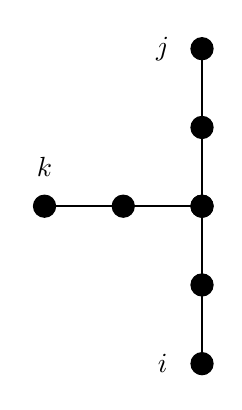
\begin{tikzpicture}
%
\draw[fill=black] (2,2) circle (4pt);
\draw[fill=black] (2,3) circle (4pt);
\draw[fill=black] (2,4) circle (4pt);
\draw[fill=black] (2,1) circle (4pt);
\draw[fill=black] (2,0) circle (4pt);
\draw[fill=black] (0,2) circle (4pt);
\draw[fill=black] (1,2) circle (4pt);
\draw[fill=black] (2,2) circle (4pt);

%
\node at (1.5,0) {$i$};
\node at (1.5,4) {$j$};
\node at (0,2.5) {$k$};
%
\draw[thick] (2,0) -- (2,4);
\draw[thick] (0,2) -- (2,2);

\end{tikzpicture}

%
\begin{caption}[1]
A $3$-armed star with arms of length $2$.
We will eventually use arms of length $t \approx \log n$.
\end{caption}
\label{fig:star}
\end{figure}


The next two lemmas check the conditions to apply Lemma~\ref{lem:basis-conditions} to the sets $\{G^\alpha\}_{\alpha \in \star_\ell(i,j,k)}$.
\begin{lemma}[Unbiased Estimator]\label{lem:block-model-unbiased-estimator}
  Let $i,j,k \in [n]$ all be distinct.
  Let $\alpha \in \star_\ell(i,j,k)$.

  For a collection of probability vectors $\sigma_1,\ldots,\sigma_k$, let $V(\sigma) = \sum_{s \in [k]} v_s^{\tensor 3}$ where $v_s(i) = \sigma_i(s) - \tfrac 1k$.
  Let $G \sim G(n,d,\e,\alpha_0,k)$.
  \[
    \E \Brac{G^\alpha \mid \sigma_i, \sigma_j, \sigma_k } = \Paren{\frac{\e d}{n}}^{3\ell} \Paren{\frac 1 {k(\alpha_0+1)}}^{3(\ell-1)} \cdot C_3 \cdot V(\sigma)_{ijk}\mper
  \]
  Here $\alpha_0 \geq 0$ is the Dirichlet concentration paramter, unrelated to the graph $\alpha$, and $C_3 = 1/(k^{O(1)} \alpha_0^{O(1)})$ is a constant related to third moments of the Dirichlet distribution.
\end{lemma}

\begin{lemma}[Approximate conditional independence]\label{lem:block-model-cond-indep}
If
  \[
  \delta \defeq 1 - \frac{k^2(\alpha_0 +1)^2}{\e^2 d} > 0 \quad \text{ and } \quad k,\alpha_0  \le n^{o(1)} \text{ and } \epsilon^2 d \le n^{o(1)} \mper
  \]
  and $\ell \geq C \log n / \delta^{O(1)}$ for a large enough constant $C$, then for $G \sim G(n,d,\e,k,\alpha_0)$,
  \[
    \E \Brac{V(\sigma)_{ijk}^2} \cdot \sum_{\alpha,\beta \in \star_\ell(i,j,k)} \E G^\alpha G^\beta \leq 1/\delta^{O(1)}\cdot \sum_{\alpha,\beta \in \star_\ell(i,j,k)} \E \Brac{G^\alpha V(\sigma)_{i,j,k}} \cdot \E \Brac{G^\beta V(\sigma)_{i,j,k}}\mper
  \]
\end{lemma}

Now we can prove Lemma~\ref{lem:mm-estimator}.
\begin{proof}[Proof of Lemma~\ref{lem:mm-estimator}]
As discussed at the beginning of this section, it is enough to find an estimator for the tensor $V(\sigma)$.
  Lemma~\ref{lem:block-model-unbiased-estimator} and Lemma~\ref{lem:block-model-cond-indep} show that Lemma~\ref{lem:basis-conditions} applies to each set of polynomials $\star_{\ell}(i,j,k)$.
  The conclusion is that for every distinct $i,j,k \in [n]$ there is a degree $\log n \poly(1/\delta)$ polynomial $P(G)_{ijk}$ so that
  \[
    \frac{\E P(G)_{ijk} V(\sigma)_{ijk}}{(\E P(G)_{ijk}^2)^{1/2} \cdot (\E V(\sigma)_{ijk}^2)^{1/2} } \geq \Omega(1)\mper
  \]
  One may check that the entries $i,j,k$ for $i,j,k$ all distinct of the tensor $V(\sigma)$ comprise nearly all of its $2$-norm.
  That is,
  \[
    \sum_{i,j,k \text{ distinct}} \E V(\sigma)_{i,j,k}^2 \geq (1 - o(1)) \E \|V(\sigma)\|^2\mper
  \]
  This is sufficient to conclude that the tensor-valued polynomial $P(G)$ whose $(i,j,k)$-th entry is $P_{i,j,k}(G)$ when $i,j,k$ are all distinct and is $0$ otherwise is a good estimator of $V(\sigma)$ (see Fact~\ref{fact:scalar-to-vector}).
  Thus,
  \[
    \frac{\E_{\sigma,G} \iprod{P(G), V(\sigma)}}
    {\Paren{\E_{\sigma,G} \Norm{P(G)}^2}^{1/2}  \cdot
    \Paren{\E_{\sigma,G} \Norm{V(\sigma)}^2}^{1/2}} \geq \Omega(1)\mper\qedhere
  \]
\end{proof}


\subsubsection{Details of unbiased estimator}
We work towards proving Lemma~\ref{lem:block-model-unbiased-estimator}.
We will need to assemble a few facts.
The first will help us control moment tensors of the Dirichlet distribution.
The proof can be found in the appendix.

\begin{fact}[Special case of Fact~\ref{fact:dirichlet-covariance}]
\label{fact:diagonal-moments}
  Let $\sigma$ be distributed according to the $\alpha,k$ Dirichlet distribution.
  Let $\tsigma = \sigma - \tfrac 1 k 1$.
  There are numbers $C_2, C_3$ depending on $\alpha,k$ so that for every $x_1, x_2, x_3$ in $\R^k$ with $\sum_{s \in [k]} x_i(s) = 0$,
  \[
    \E_\sigma \iprod{\tsigma, x_1}\iprod{\tsigma, x_2}   = C_2 \iprod{x_1, x_2}
  \]
  and
  \[
    \E_\sigma \iprod{\tsigma, x_1}\iprod{\tsigma, x_2}\iprod{\tsigma,x_3} = C_3 \sum_{s \in [k]} x_1(s) x_2(s) x_3(s)\mper
  \]
  Furthermore,
  \[
    C_2 = \frac 1 {k(\alpha + 1)} \quad \text{ and } \quad C_3 = \frac 1 {k^{O(1)} \alpha^{O(1)}}\mper
  \]
\end{fact}

Now we can prove Lemma~\ref{lem:block-model-unbiased-estimator}.
\begin{proof}[Proof of Lemma~\ref{lem:block-model-unbiased-estimator}]
  For any collection of $\sigma$'s and $\alpha \in \star_\ell(i,j,k)$,
  \begin{align*}
    \E_{G} \Brac{G^\alpha \mid \sigma} & = \Paren{\frac{\epsilon d}{n}}^{3\ell} \prod_{(a,b) \in \alpha} \iprod{\tsigma_a,\tsigma_b}
  \end{align*}
  Let $a$ be the central vertex of the star $\alpha$.
  Taking expectations over all the vertices in the arms of the star,
  \[
  \E \Brac{G^\alpha \mid \sigma_i, \sigma_j, \sigma_k } = \Paren{\frac{\epsilon d}{n}}^{3\ell} \Paren{\frac 1 {k(\alpha_0 +1)}}^{3(\ell-1)} \E_{\sigma_a} \iprod{\tsigma_i,\tsigma_a} \iprod{\tsigma_j,\tsigma_a} \iprod{\tsigma_k,\tsigma_a}\mper
  \]
  Finally, using the second part of Fact~\ref{fact:diagonal-moments} completes the proof.
\end{proof}

\subsubsection{Details of approximate conditional independence}
We prove Lemma~\ref{lem:block-model-cond-indep}, first gathering some facts.
In the sum $\sum_{\alpha, \beta \in \star_\ell(i,j,k) } G^\alpha G^\beta$, the terms $\alpha, \beta$ which (as graphs) share only the vertices $i,j,k$ will not cause us any trouble, because such $G^\alpha$ and $G^\beta$ are independent conditioned on $\sigma_i, \sigma_j, \sigma_k$.
\begin{fact}\label{fact:mm-indep}
  If $\alpha, \beta \in \star_\ell(i,j,k)$ share only the vertices $i,j,k$, then for any collection $\sigma$ of probability vectors,
  \[
    \E\Brac{ G^\alpha G^\beta  \mid \sigma_i, \sigma_j, \sigma_k} = \E \Brac{ G^\alpha \mid \sigma_i, \sigma_j, \sigma_k} \cdot \E \Brac{ G^\beta \mid \sigma_i, \sigma_j, \sigma_k}\mper
  \]
\end{fact}
\begin{proof}
  To sample $G^\alpha$, one needs to know $\sigma_a$ for any $a \in [n]$ with nonzero degree in $\alpha$, and similar for $b \in [n]$ and $G^\beta$.
  The only overlap is $\sigma_i, \sigma_j, \sigma_k$.
\end{proof}

The next fact is the key one.
Pairs $\alpha, \beta$ which share vertices forming paths originating at $i,j,$ and $k$ make the next-largest contribution (after $\alpha, \beta$ sharing only $i,j,k$) to $\sum_{\alpha, \beta} \E G^\alpha G^\beta$.
\begin{fact}\label{fact:mm-path-intersection}
  Let $i,j,k \in [n]$ be distinct.
  Let $V(\sigma)_{ijk}$ be as in the Lemma~\ref{lem:block-model-cond-indep}.
  Let $C_2 \in \R$ be as in Fact~\ref{fact:diagonal-moments}.

  Let $\alpha, \beta \in \star_\ell(i,j,k)$ share $s$ vertices (in addition to $i,j,k$) for some $s \leq \tfrac t 2$, and suppose the shared vertices form paths in $\alpha$ and $\beta$ starting at $i, j, $ and $k$.
  Then
  \[
    \E V(\sigma)_{ijk}^2 \cdot \E G^\alpha G^\beta \leq \e^{-2s} \Paren{\frac{ d} n}^{-s} (1 + O(d/n))^{-s} \cdot \Paren{\frac 1 {k(\alpha_0+1)}}^{-2s} \cdot \E\Brac{ G^{\alpha} V(\sigma)_{ijk}} \cdot \E \Brac{G^{\beta} V(\sigma)_{ijk}} \mper
  \]
\end{fact}
\begin{proof}
  Let $\sigma_{\alpha \cap \beta}$ be the $\sigma$'s corresponding to vertices sharerd by $\alpha, \beta$.
  Let $i', j', k'$ be the last shared vertices along the paths beginning at $i,j,k$ respectively.
  We expand $G^\alpha G^\beta$ and use conditional independence of the $G_e$'s given the $\sigma$'s:
  \[
    \E G^\alpha G^\beta = \E_{\sigma_{i', j', k'} }\Brac{ \E \Brac{ (G^{\alpha \cap \beta})^2 \, | \sigma_{i'}, \sigma_{j'}, \sigma_{k'}} \cdot \E \Brac{G^{\alpha \setminus \beta} \mid \sigma_{i'} \sigma_{j'} \sigma_{k'}} \cdot \E \Brac{G^{\beta \setminus \alpha } \mid \sigma_{i'} \sigma_{j'} \sigma_{k'}}} \mper
  \]
  Both $G^{\alpha \setminus \beta}$ and $G^{\beta \setminus \alpha}$ are long-armed stars with terminal vertices $i', j', k'$.
  The arm lengths of $G^{\alpha \setminus \beta}$ total $3\ell - s$.
  By a similar argument to Lemma~\ref{lem:block-model-unbiased-estimator}, $G^{\alpha \setminus \beta}$ is an unbiased estimator of $V(\sigma)_{i'j'k'}$ with
  \[
    \E\Brac{G^{\alpha \setminus \beta} \mid \sigma_{i'}, \sigma_{j'}, \sigma_{k'}}
    = \Paren{\frac {\e d}n}^{3\ell -s} \Paren{\frac 1 {k(\alpha_0 +1)}}^{3(\ell -1) -s} \cdot C_3 \cdot V(\sigma)_{i', j', k'}
  \]
  and the same goes for $G^{\beta \setminus \alpha}$.
  Furthermore,
  \[
    \E \Brac{ (G^{\alpha \cap \beta})^2 \mid \sigma_{i'}, \sigma_{j'}, \sigma_{k'}}
    = \Paren{\frac dn}^{|\alpha \cap \beta|} \E \Brac{\prod_{(a,b) \in \alpha \cap \beta} (1 + \e \iprod{\tsigma_a, \tsigma_b} + O(d/n)) \, \Big{|} \, \sigma_{i'}, \sigma_{j'}, \sigma_{k'}}\mper
  \]
  By our assumption that $\alpha \cap \beta$ consists just of paths, every subset of edges in the graph $\alpha \cap \beta$ contains a vertex of degree $1$.
  Hence, $\E \Brac{ (G^{\alpha \cap \beta})^2 \mid \sigma_{i'}, \sigma_{j'}, \sigma_{k'}} = (1 + O(d/n))^{|\alpha \cap \beta|} (d/n)^{|\alpha \cap \beta|}$.
  Putting these together,
  \[
    \E G^\alpha G^\beta = (1 + O(d/n))^s \e^{6\ell - 2s} \Paren{\frac dn}^{6\ell - s} \Paren{\frac 1 {k(\alpha_0 +1)}}^{6(\ell-1) - 2s} C_3^2 \E V(\sigma)_{ijk}^2
  \]
  At the same time, one may apply Lemma~\ref{lem:block-model-unbiased-estimator} to $\E G^{\alpha} V(\sigma)_{ijk}$ to obtain
  \[
    \E\Brac{ G^{\alpha} V(\sigma)_{ijk}} \cdot \E \Brac{G^{\beta} V(\sigma)_{ijk}}
    = \Paren{\frac {\e d}n}^{6\ell} \Paren{\frac 1 {k(\alpha_0 + 1)}}^{6(\ell-1)} C_3^2 \cdot \Paren{\E_{\sigma_{i},\sigma_{j}, \sigma_{k}} V(\sigma)_{ijk}^2}^2 \mper
  \]
  The lemma follows.
\end{proof}

The last fact will allow us to control $\alpha, \beta$ which intersect in some way other than paths starting at $i,j,k$.
The key idea will be that such pairs $\alpha, \beta$ must share more vertices than they do edges.
\begin{fact}\label{fact:mm-nonpath-intersection}
  Let $i,j,k \in [n]$ be distinct.
  Let $V(\sigma)_{ijk}$ be as in the Lemma~\ref{lem:block-model-cond-indep}.
  Let $C_2 \in \R$ be as in Fact~\ref{fact:diagonal-moments}. $C_2 = \tfrac 1 {k(\alpha_0+1)}$.

  Let $\alpha, \beta \in \star_\ell(i,j,k)$ share $s$ vertices (in addition to $i,j,k$) and $r$ edges.
  Then
  \[
    \E V(\sigma)_{ijk}^2 \cdot \E G^\alpha G^\beta \leq \e^{-2r} \Paren{\frac dn}^{-r} \cdot C_2^{-2s} \cdot k^{O(s-r)} (1+\alpha_0)^{O(s-r)} \cdot \E\Brac{ G^{\alpha} V(\sigma)_{ijk}} \cdot \E \Brac{G^{\beta} V(\sigma)_{ijk}} \mper
  \]
\end{fact}
\begin{proof}
  Expanding as usual,
  \begin{align*}
  \E G^{\alpha} G^{\beta} = \Paren{\frac dn}^{6\ell - r} \E_\sigma \prod_{ab \in \alpha \triangle \beta} \iprod{\tsigma_a,\tsigma_b} \cdot \prod_{ab \in \alpha \cap \beta} (1 + \e \iprod{\tsigma_a,\tsigma_b} + O(d/n))\mper
  \end{align*}
  Any nontrivial edge-induced subgraph of $\alpha \cap \beta$ contains a degree-1 vertex; using this to expand the second product and simplifying with $\E \tsigma_a = 0$, the above is
  \[
    \Paren{\frac dn}^{6\ell - r} \E_\sigma \prod_{ab \in \alpha \triangle \beta} \iprod{\tsigma_a,\tsigma_b} \cdot (1 + O(d/n))^{r}\mper
  \]
  For every degree-2 vertex in $\alpha \triangle \beta$ we can use Fact~\ref{fact:dirichlet-covariance} to take the expectation.
  Each such vertex contributes a factor of $C_2$ and there are at least $3\ell - O(s-r)$ such vertices.
  The remaining expression will be bounded by $1$.
  The fact follows.
\end{proof}

Now we can prove Lemma~\ref{lem:block-model-cond-indep}.
\begin{proof}[Proof of Lemma~\ref{lem:block-model-cond-indep}]
  Let us recall that our goal is to show
  \[
    \E \Brac{V(\sigma)_{ijk}^2} \cdot \sum_{\alpha,\beta \in \star_\ell(i,j,k) } \E G^\alpha G^\beta \leq \delta^{O(1)} \cdot \sum_{\alpha,\beta \in \star_\ell(i,j,k)} \E \Brac{G^\alpha V(\sigma)_{ijk}} \cdot \E \Brac{G^\beta V(\sigma)_{ijk}}
  \]
  where $\delta = 1 - \tfrac{k^2 (\alpha_0 +1)^2}{\e^2 d}$.
  Let $c = \E \Brac{G^\alpha V(\sigma)_{ijk}} \cdot \E \Brac{G^\beta V(\sigma)_{ijk}}$.
  (Notice this number does not depend on $\alpha$ or $\beta$.)
  The right-hand side above simplifies to $|\star_\ell(i,j,k)|^2 \cdot c$.

  On the left-hand side, what is the contribution from $\alpha,\beta$ sharing $s$ vertices?
  First consider what happens with $s \leq t/2$ and the intersecting vertices form paths in $\alpha$ and $\beta$ starting at $i,j,k$.
  Choosing a random pair $\alpha, \beta$ from $\star_\ell(i,j,k)$, the probability that they intersect along paths of length $s_1, s_2, s_3$ starting at $i,j,k$ respectively is at most $n^{-s_1 - s_2 - s_3}$.
  There are at most $(1 + s^2)$ choices for nonnegative integers $s_1,s_2,s_3$ with $s_1 + s_2 + s_3 = s$.
  By Fact~\ref{fact:mm-path-intersection}, such terms therefore contribute at most
  \[
    c \cdot \frac{|\star_\ell(i,j,k)|^2}{n^{-s}} \cdot \Paren{\epsilon \sqrt{\tfrac d n}(1 + O(d/n))}^{-2s} C_2^{-2s} \cdot s^2
    = c \cdot |\star_\ell(i,j,k)|^2 \cdot (\epsilon^2 d C_2^2 (1 + O(d/n)))^{-s} \cdot s^2
  \]
  where $C_2 = \tfrac 1 {k(\alpha_0 +1)}$.
By hypothesis, $\delta > 0$.
  Consider the sum of all such contributions for $s \leq t/2$; this is at most
  \[
    c \cdot |\star_\ell(i,j,k)|^2 \cdot \sum_{s = 0}^{t/2} (1 + s^2) \cdot \Paren{\tfrac{k^2(\alpha_0+1)^2}{\e^2 d}}^{s} \leq \delta^{O(1)} \cdot c \cdot |\star_\ell(i,j,k)|^2 \mper
  \]

  Next, consider the contribution from $\alpha, \beta$ which share $s$ vertices in some pattern other than those considered above.
  Unless $\alpha = \beta$, this means $\alpha, \beta$ share at least one more vertex than the number $r$ of edges that they share.
  Suppose $\alpha \neq \beta$ and let $s - r = q$.
  There are $t^{O(q)}$ patterns in which such an intersection might occur, and each occurs for a random pair $\alpha, \beta \in \star_\ell(i,j,k)$ with probabilty $n^{-s}$.
  So using Fact~\ref{fact:mm-nonpath-intersection}, the contribution is at most
  \[
    c \cdot |\star_\ell(i,j,k)|^2 \cdot \sum_{q = 1}^{t} \Paren{\frac{\epsilon^2 d}{n}}^q \cdot k^{O(q)} (1+\alpha_0)^{O(q)} t^{O(q)}
  \]
By the hypotheses $k, \alpha = n^{o(1)}$ and $\epsilon^2 d = n^{1 - \Omega(1)}$, this is all $o(c |\star_\ell(i,j,k)|^2)$.

  Finally, consider the case $\alpha = \beta$.
  Then, using Fact~\ref{fact:mm-nonpath-intersection} again, the contribution is at most
  \[
    c \cdot |\star_\ell(i,j,k)|^2 \Paren{\frac{\epsilon^2 d}{k^2 (\alpha_0 + 1)^2}}^{-t} k^{O(1)} \alpha^{O(1)}
  \]
  which is $o(c |\star_\ell(i,j,k)|^2)$ because $t \gg \log(n)$.
  Putting these things together gives the lemma.
\end{proof}

\subsection{Cross validation}
\Snote{}
In this section we show how to use a holdout set of vertices to cross-validate candidate community membership vectors.
The arguments are all standard, using straightforward concentration inequalities.
At the end we prove the first part of Lemma~\ref{lem:xvalid-est}, on the estimator $S_3$.
The proof of the second part, on $S_4$ is similar, using standard facts about moments of the Dirichlet distribution (see Fact~\ref{fact:dirichlet-covariance}).
The proof of Lemma~\ref{lem:xvalid-est-orth} is also similar, using the discussion in Section~\ref{sec:estimator-third-moment} to turn estimators for moments of the $v$ vectors into estimators for moments of the $w$ vectors---we leave it to the reader.

We will need a few facts to prove the lemma.
\begin{fact}
  \label{fact:xvalid-1}
  Let $n_0,n_1,A,k,d,\e,\alpha,\sigma,v,\tau,G,x,P$ be as  in Lemma~\ref{lem:xvalid-est}.
  Let $a \in A$.
  There is a number $C = C(k,\alpha) \leq \poly(k,\alpha)$ such that
  \begin{align*}
  \E_{G,\tau} P_a(G,x)  = \Paren{ \frac{\e d}{n}}^3 \cdot C \cdot \sum_{ijk \in \overline{A} \text{ distinct}} \sum_{s \in [k]} \sigma_i(s) \sigma_j(s) \sigma_k(s) x_i x_j x_k\mper
  \end{align*}
\end{fact}
\begin{proof}
  Immediate from Fact~\ref{fact:diagonal-moments}.
\end{proof}

\begin{fact}
  \label{fact:xvalid-2}
  Let $n_0,n_1,A,k,d,\e,\alpha,\sigma,v,\tau,G,x,P$ be as  in Lemma~\ref{lem:xvalid-est}.
  Let $a \in A$.
  The following variance bound holds.
  \[
    \E_{G,\tau} P_a(G,x)^2 - \Paren{\E_{G,\tau} P_a(G,x)}^2 \leq \frac{\poly(k,\alpha,\e,d)}{n^{3}}\mper
  \]
\end{fact}
\begin{proof}
  Expanding $P_a(G,x)$ and using that $|\iprod{\sigma,\sigma'}| \leq 1$ for any $\sigma, \sigma' \in \Delta_{k-1}$ we get
  \[
    \E_{G,\tau} P_a(G,x)^2  \leq \Paren{\frac{d}{n}}^6 \sum_{\substack{ijk \text{ distinct}\\{i'j'k' \text{ distinct}}}} \Abs{x_i x_j x_k x_{i'} x_{j'} x_{k'} } \leq \Paren{\frac{d}{n}}^6 \cdot n^3 \cdot \|x\|^{12}\mper
  \]
\end{proof}

\begin{fact}
  \label{fact:xvalid-3}
  Let $n_0,n_1,A,k,d,\e,\alpha,\sigma,v,\tau,G,x,P$ be as  in Lemma~\ref{lem:xvalid-est}.
  Let $a \in A$.
  For some constant $\gamma_*(\e,d,k,\alpha)$ and every $\gamma_* > \gamma > 0$,
  \[
    \Pr_{G,\tau} \left \{ |P_a(G,x)| > n^{\gamma} \right \} \leq \exp(-n^{\Omega(\gamma)})
  \]
\end{fact}
\begin{proof}
  The fact follows from a standard exponential tail bound on the degree of vertex $a$.
\end{proof}

We can put these facts together to prove the $S_3$ portion of Lemma~\ref{lem:xvalid-est} (as we discussed above, the $S_4$ portion and Lemma~\ref{lem:xvalid-est-orth} are similar).
The strategy will be to use the following version of Bernstein's inequality, applied to the random variables $\iprod{G_a, v^{\tensor 3}}$.
The proof of the inequality is in the appendix.
\begin{proposition}[Bernstein wth tails]\label{prop:bernstein-tails}
  Let $X$ be a random variable satisfying $\E X = 0$ and, for some numbers $R,\delta,\delta' \in \R$,
  \[
    \Pr \{ |X| > R \} \leq \delta \text{ and } \E|X|\cdot \Ind_{|X| > R} \leq \delta'\mper
  \]
  Let $X_1,\ldots,X_m$ be independent realizations of $X$.
  Then
  \[
    \Pr \left \{ \Abs{\tfrac 1 m \sum_{i \leq m} X_i} \geq t + \delta' \right \} \leq \exp\Paren{\frac{- \Omega(1) \cdot m \cdot t^2}{\E X^2 + t\cdot R}} + m \delta \mper
  \]
\end{proposition}

Now we can prove Lemma~\ref{lem:xvalid-est}.

\begin{proof}[Proof of Lemma~\ref{lem:xvalid-est}]
  We apply Proposition~\ref{prop:bernstein-tails} to the $n_1$ random variables $X_a = \Paren{\tfrac{\e d} n}^{-3} C^{-1} P_a(G,x)$ for $a \in A$, where $C = C(k,\alpha)$ is the number from Fact~\ref{fact:xvalid-2}.
  (For each $a \in A$ these are iid over $G,\tau$.)
  Take $t = n^{3/2 - \gamma'}$ for a small-enough constant $\gamma'$ so that $n_1t^2/n^3 \geq n^{\gamma}$ for some constant $\gamma$, using the assumption $n_1 \geq n^{\Omega(1)}$.
  All together, we get
  \[
  \Pr_{G,\tau} \left \{ \Abs{\frac 1 {n_1} \sum_{a \in A} X_a - \sum_{s \in [k]} \sum_{ijk \in \overline A \text{ distinct}} \sigma_s(i) \sigma_s(j) \sigma_s(k) x_i x_j x_k } \geq n^{3/2 - \gamma'} \right \} \leq \exp(n^{-\gamma'})
  \]
  for some constants $\gamma, \gamma'$ (possibly different from $\gamma, \gamma'$ above) and large-enough $n$.
  For any unit $x \in \R^{n_0}$ and $\sigma \in \Delta_{k-1}^{n_0}$, using that $k \leq n^{o(1)}$ it is not hard to show via Cauchy-Schwarz that
  \[
  \Abs{\sum_{s \in [k]} \iprod{v_s,x}^3 - \sum_{s \in [k]} \sum_{ijk \in \overline A \text{ distinct}} \sigma_s(i) \sigma_s(j) \sigma_s(k) x_i x_j x_k} \leq n^{1 + o(1)}\mper
  \]
  The lemma follows.
\end{proof}

\subsection{Producing probability vectors}
\newcommand{\ov}{\overline{v}}
\newcommand{\ow}{\overline{w}}

In this section we prove Lemma~\ref{lem:cleanup}.
The proof of Lemma~\ref{lem:cleanup-2} is very similar (in fact it is somewhat easier) so we leave it to the reader.
\restatelemma{lem:cleanup}
 First some preliminaries.
Let $\sigma_1,\ldots,\sigma_n$ be iid from the $\alpha,k$ Dirichlet distribution.
There are two important families of vectors in $\R^n$.
Let
\[
v_s(i) = \sigma_i(s) - \frac 1k \qquad w_s(i) = \sigma_i(s) - \frac 1k\Paren{1 - \frac 1 {\sqrt{\alpha+1}}}\mper
\]
We will also work with a normalized version of the $v$ vectors:
\[
  \overline{v}_s = \frac{v_s}{(\E\|v_s\|^2)^{1/2}}\mper
\]
By construction, $\E\|\overline{v}_s\|^2 = 1$.
Also by definition, $\sum_s v_s = \sum_s \overline{v}_s = 0$.
Thus $\E \iprod{\sum_s \ov_s ,\sum_s \ov_s} = k + \sum_{s \neq t} \E\iprod{\ov_s,\ov_t} = 0$ and so by symmetry $\E \iprod{\ov_s,\ov_t} = \frac{-1}{k-1}$.
We let
\[
\ow_s = \ov_s + \frac 1{\sqrt n} \cdot \sqrt{\frac 1 {k-1}}
\]
so that $\E \iprod{\ow_s,\ow_t} = 0$ for $s \neq t$.
(In the facts which follow we sometimes write $\ov$ as $v$ when both normalizations are not needed; this is always noted.)

We will want the following fact; the proof is elementary.
\begin{fact}\label{fact:v-corr}
  Let $\sigma,u,v,w$ as above, and suppose $y$ is an $n \times k$ matrix whose rows are in $\Delta_{k-1} - \tfrac 1k$ (that is they are shifted probability vectors).
  Then $\tau = y + \tfrac 1k$ is a matrix whose rows are probability vectors, and $\tau$ satisfies
  \[
    \iprod{\tau,\sigma} \geq \iprod{y,v} + \frac nk\mper
  \]
\end{fact}

The following fact will be useful when $\delta$ is small but not tiny; i.e. $\delta < 1 - c$ for some fixed constant $c$ but $\delta \gg 1/\sqrt k$.
\begin{fact}
\label{fact:permutation-small}
  Suppose that $x_1,\ldots,x_k$ are unit vectors and $w_1,\ldots,w_k$ are orthonormal.
  Also suppose that there is $1 > \delta > 0$ such that for at least $\delta k$ vectors $w_s$ among $w_1,\ldots,w_k$ there exists a vector $x_t$ among $x_1,\ldots,x_k$ such that $\iprod{w_s,x_t} \geq \delta$.
  Then there is a permutation $\pi : [k] \rightarrow [k]$ such that if $x = (x_1,\ldots,x_k)$ is an $n \times k$ matrix and similarly for $w$,
  \[
  \iprod{x, \pi \cdot w} \geq \Paren{\delta^5 - \frac 1 {\sqrt k}\Paren{\frac 1 {1-\delta^4}}^{1/2}} \|x\|\|w\|\mcom
  \]
  where $x = (x_1,\ldots,x_k)$ is an $n \times k$ matrix and similarly for $w$.
\end{fact}
\begin{proof}
  We will think of $\pi$ as a matching of $w_1,\ldots,w_k$ to $x_1,\ldots,x_k$.
  Call $x_t$ \emph{good} for $w_s$ if $\iprod{w_s,x_t} \geq \delta$.
  First of all, by orthogonality of vectors $w_1,\ldots,w_k$, any particular vector $x_t$ is good for at most $1/\delta^2$ vectors $w_s$.
  Hence, there is a set $S$ of $\delta^4 k$ vectors $w_s$ such that for each $w_s$ there exists a good $x_t$ and all the good $x_t$'s are distinct.

  Begin by matching each $w_s \in S$ to its good $x_t$.
  Let $\pi$ be the result of extending that matching randomly to a perfect matching of $k$ to $k$.

  We need to lower bound $\E \sum_{s \notin S} \iprod{w_s,x_{\pi (s)}}$.
  Consider that for a particular $t$,
  \[
  \E -\iprod{x_t, w_{\pi^{-1}(t)}} \leq (\E \iprod{x_t, w_{\pi^{-1}(t)}}^2)^{1/2}\mper
  \]
  The distribution of $\pi^{-1}(t)$ is uniform among all $s \notin S$.
  So
  \[
    \E \iprod{x_t, w_{\pi^{-1}(t)}}^2 = \frac 1 {k - |S|} \sum_{s \notin S} \iprod{w_s,x_t}^2 \leq \frac 1k \Paren{\frac 1 {1 - \delta^4}}
  \]
  since $\sum_{s \in [k]} \iprod{w_s,x_t}^2 \leq 1$.
  It follows that
  \[
    \E \iprod{x_t, w_{\pi^{-1}(t)}} \geq - \frac 1 {\sqrt k} \Paren{\frac 1 {1-\delta^4}}^{1/2}\mper
  \]
  Therefore, $\E \sum_{s \notin S} \iprod{w_s, x_{\pi(s)}} \geq - \sqrt k\Paren{\frac 1 {1-\delta^4}}^{1/2}$.
  Thus there is some choice of $\pi$ such that $\sum_{s \notin S} \iprod{w_s, x_{\pi(s)}} \geq - \sqrt k\Paren{\frac 1 {1-\delta^4}}^{1/2}$.
  Hence for this $\pi$ one gets
  \[
    \sum_{s \in [k]} \iprod{w_s,x_{\pi(s)}} \geq \delta^5 k - \sqrt k\Paren{\frac 1 {1-\delta^4}}^{1/2} = \Paren{\delta^5 - \frac 1 {\sqrt k}\Paren{\frac 1 {1-\delta^4}}^{1/2}} \|x\|\|w\|\mper\qedhere
  \]
\end{proof}

The next fact serves the same purpose as the previous one but in the large $\delta$ case (i.e. $\delta$ close to $1$).
\begin{fact}
\label{fact:permutation-large}
  Under the same hypotheses as Fact~\ref{fact:permutation-small}, letting $\delta = 1 - \e$ for some $\e > 0$, there is a permutation $\pi : [k]  \rightarrow [k]$ such that $\iprod{x,\pi \cdot w} \geq (1 - 9\e) \|x\|\|w\|$.
\end{fact}
\begin{proof}
  As in the proof of Fact~\ref{fact:permutation-small}, we construct a matching $\pi$ by first matching a set $S$ of at least $\delta^4k \geq (1 - 4\e)k$ vectors $w_s$ to corresponding $x_t$.
  Then we match the remaining vectors arbitrarily.
  For any $s,t$ we know $\iprod{w_s,x_t} \geq -1$.
  So the result is
  \[
  \iprod{x, \pi \cdot w} \geq (1 - 5 \e) k - 4 \e k = (1 - 9 \e) k = (1 - 9\e) \|x\|\|w\|\mper\qedhere
  \]
\end{proof}

We will also want a way to translate a matrix correlated with $w$ to one correlated with $v$, so that we can apply Fact~\ref{fact:v-corr}.
\begin{fact}
  \label{fact:shift-1}
  Suppose $v$ is an $n \times k$ matrix whose rows are centered probability vectors and $w = v + c$ is a coordinate-wise additive shift of $v$.
  Suppose $y$ is also an $n \times k$ matrix whose rows are centered probability vectors shifted by $c$ in each coordinate (so $y - c$ is a matrix of centered probability vectors).
  Then the shifted matrix $y-c$ satisfies
  \[
    \iprod{y-c,v} \geq \iprod{y,w} - c^2 nk\mper
  \]
\end{fact}
\begin{proof}
  By definition, $\iprod{y -c,v} = \iprod{y,v}$. Since $v = w -c$, we get
  \[
    \iprod{y-c,v} = \iprod{y,v} = \iprod{y,w} - c \iprod{y, 1} = \iprod{y,w} - c^2 nk\mper\qedhere
  \]
\end{proof}

\begin{proof}[Proof of Lemma~\ref{lem:cleanup}]
  First assume $\delta < 1 - c$ for any small constant $c$.
  Let $\pi$ be the permutation guaranteed by Fact~\ref{fact:permutation-small} applied to the vectors $x_1,\ldots,x_k$ and $M^{-1/2}w_1,\ldots,M^{-1/2}w_k$.
  (Without loss of generality reorder the vectors so that $\pi$ is the identity permutation.)
  Since $1-c \geq \delta \geq 1/k^{1/C}$ for big-enough $C$ and small-enough $c$ (which are independent of $n,k$) and the guarantee of Fact~\ref{fact:permutation-small}, by event $E$ we get that
  \[
    \iprod{x,w} \geq \delta^{O(1)} \|x\| \|w\|\mper
  \]
  So by taking a correlation-preserving projection of $x$ into the set of matrices whose rows are shifted probability vectors, we get a matrix $y$ with the guarantee
  \[
  \iprod{y,w} \geq \delta^{O(1)} \|y\| \|w\| \quad \text{ and } \quad \|y\| \geq \delta^{O(1)} \|w\|\mper
  \]
  Applying Fact~\ref{fact:shift-1}, we obtain
  \[
  \iprod{y -c,v} \geq \iprod{y,w} - c^2 nk = \iprod{y,w} - \frac{\E \|w\|^2}{k}
  \]
  where $c = \tfrac 1 {k \sqrt{\alpha+1}}$.
  Putting things together and using $\E \|v\|^2 \leq \E \|w\|^2$ and the event $E$, we get
  \[
    \iprod{y-c,v} \geq \delta^{O(1)} \E\|v\|^2\mper
  \]
  So applying Fact~\ref{fact:v-corr} finishes the proof in this case.

  Now suppose $\delta \geq 1 -c$ for a small-enough constant $c$.
  Then using event $E$ and Fact~\ref{fact:permutation-large}, there is $\pi$ such that $\iprod{x,w} \geq (1 - O(c)) \|x\|( \E \|w\|^2)$ (where again we have without loss of generality reordered the vectors so that $\pi$ is the identity permutation).
 Now taking the Euclidean projection of $x \cdot \frac{(\E \|w\|^2)^{1/2}}{\|x\|}$ into the $n \times k$ matrices whose rows are centered probability vectors shifted entrywise by $c = \tfrac 1 {k\sqrt{\alpha+1}}$, we get a matrix $y$ which again satisfies
 $\iprod{y,w} \geq (1 - O(c)) \|y\|\|w\|$ and $\|y\| \geq (1 - O(c)) \|w\|$, so (using event $E$), $\iprod{y,w} \geq (1 - O(c)) \E \|w\|^2$.
 Removing the contribution from $\iprod{y,1}$, this implies that $\iprod{y-c,v} \geq (1 - O(c)) \E \|v\|^2$.
 For $c$ small enough, this is at least $\delta^{O(1)} \E \|v\|^2$.
 Applying Fact~\ref{fact:v-corr} finishes the proof.
\end{proof}


\subsection{Remaining lemmas}
We provide sketches of the proofs of Lemma~\ref{lem:shift-and-whiten} and Lemma~\ref{lem:cleanup}, since the proofs of these lemmas use only standard techniques.

\begin{proof}[Proof sketch of Lemma~\ref{lem:shift-and-whiten}]
  For $\sigma \in \R^k$, let $\tilde{\sigma} = \sigma - (1 - 1/\sqrt{\alpha+1})/k$.
  Standard calculations show that if $\sigma$ is drawn from the $\alpha,k$ Dirichlet distribution then $\E \tsigma \tsigma^\top = \tfrac 1 {k(\alpha+1)} \Id$.
  It follows by standard matrix concentration and the assumption $k,\alpha \leq n^{o(1)}$ that the eigenvalues of $\frac 1n \sum_{i \leq n} \tsigma_i \tsigma_i^\top$ are all $1 \pm n^{-\Omega(1)}$, where $\sigma_1,\ldots,\sigma_n$ are iid draws from the $\alpha,k$ Dirichlet distribution.

  For the second part of the Lemma, use the first part to show that $\Norm{\tfrac{v_s}{\|v_s\|} - w'_s} \leq 1/\poly(k)$.
  Then when $k \geq \delta^{-C}$ for large-enough $C$, if $\iprod{x,v_s}^3 \geq \delta^{O(1)} \|v_s\|^3$ it follows that also $\iprod{x,w_s} \geq \delta^{O(1)} - 1/\poly(k) \geq \delta^{O(1)}$.
  The lemma follows.
\end{proof}

\begin{proof}[Proof sketch of Lemma~\ref{lem:cleanup}]
  If $\delta < 1 - \Omega(1)$, then $\delta^2/2 \geq \delta^{O(1)}$, so the Lemma follows from standard concentration and Theorem~\ref{thm:correlation-preserving-projection} on correlation-preserving projection.
  On the other hand, if $\delta \geq 1 - o(1)$, then $\|v' - \tsigma\| \leq o(1) \cdot \|\tsigma\|$, so the same is also true for the projection of $v'$ into $(\tilde{\Delta}_{k-1})^n$ by convexity and the lemma follows.
\end{proof}




\iffalse


We work with very sparse graphs---essentially they are samples from $G(n,d,\e, \alpha,k)$ where $\epsilon^2 d > \eta \cdot k^2 (\alpha + 1)^2$ for some constant $\eta > 0$.
(This is as opposed to the setting for recovery, when $\epsilon^2 d > (1 + \Omega(1)) k^2 (1 + \alpha)$.)
To ensure that we are using fresh randomness in the cross validation we have to condition on the partition $H_1, H_2$.
This means the graph we use in this step will not exactly have the block model distribution, but the estimation facts we need will still hold.

Our main tool to prove Lemma~\ref{lem:xvalid-main} will be the following.



\begin{lemma}\label{lem:xvalid-main-estimator}
  Let $G$ be the holdout graph as in the partial recovery algorithm, with expected average degree $h$.
  Suppose $\epsilon^2 h > \eta k^2 (k\alpha + 1)^2$ for some $\eta = \Omega(1)$.
  Suppose $k, \alpha, \epsilon^2 h \leq n^{o(1)}$

  Let $A, \overline A$ be a random patition of $[n]$ into two sets of size $\tfrac n 2$.
  Let $v_s \in \R^{\overline A}$ for $s \in [k]$ be the vectors $v_s(i) = \sigma_i(s) - \tfrac 1 k$ for $i \in \overline A$.
  Let $v \in \R^{\overline A}$ be a unit vector with $|v(i)| \leq n^{-1/2 + o(1)}$ for each coordinate $i \in \overline A$.

  For $a \in A$, let $H_a$ be the $3$-tensor indexed by $i,j,k \in \overline A$ with $(H_a)_{i,j,k} = H_{ai}H_{aj}H_{ak}$ when $i,j,k$ are all distinct and the pairs $(i,a), (j,a), (k,a)$ all belong to $H_2$, and $0$ otherwise.
  Here $H_{ab}$ is the centered indicator $H_{ab} = x_{ab} - \tfrac dn$.

  There is a number $c$ so that with probability at least $1-n^{-\omega(1)}$, conditioned on $H_1$ and $H_2$,
  \[
    \Abs{\frac 1 {c |A|} \sum_{a \in A} \iprod{H_a, v^{\tensor 3}} - \sum_{s \in [k]} \iprod{v_s, v}^3} \leq n^{3/2 - \Omega(1)}\mper
  \]
\end{lemma}

From this we can prove Lemma~\ref{lem:xvalid-main}

\begin{proof}[Proof of Lemma~\ref{lem:xvalid-main}]
  First suppose that the unit vector $x$ has some coordinates with $|x(i)| > n^{-1/2 + \Omega(1)}$.
  Let $S \subseteq [n]$ be the set of such coordinates.
  Since $x$ is a unit vector, there can only be $n^{1-\Omega(1)}$ such coordinates.
  The vectors $v_s$ all have (with high probability) all coordinates bounded by $n^{-1/2 + o(1)}$ in magnitude.
  So, for any $v_s$,
  \[
    \Abs{\sum_{i \in [S]} v_s(i) x(i) } \leq \Paren{\sum_{i \in S} v_s(i)^2}^{1/2} \leq n^{-\Omega(1)}
  \]
  Setting all such coordinates of $x$ to zero affects $\iprod{x,v_s}$ be only $n^{-\Omega(1)}$ additively, so we assume $x$ has all coordinates at most $n^{-1/2 + o(1)}$ in magnitude.

  The oracle computes the value of the estimator from Lemma~\ref{lem:xvalid-main-estimator}, obtaining a number
  \[
    a = \frac 1 {(\E \|v_s\|^2)^{3/2}} \sum_{s \in [k]} \iprod{v_s,x}^3 \pm n^{-\Omega(1)}\mper
  \]
  The norms $\|v_s\|^2$ are highly concentrated (this can be proved via standard techniques).
  The lemma follows.
\end{proof}


For the remainder of the section we turn to proving Lemma~\ref{lem:xvalid-main-estimator}.
The proof will re-use many of the ideas from previous sections.
First, we show that the $G_a$'s are unbiased estimators of (the multilinear part of) $\sum_{s \in [k]} v_s^{\tensor 3}$.

\begin{lemma}\label{lem:xvalid-unbiased-estimator}
  Consider the same setup as in Lemma~\ref{lem:xvalid-main-estimator}.
  Let
  \[
    f(v) = \sum_{s \in [k]} \sum_{i,j,k \in \overline A \text{ all distinct}} v(i) v(j) v(k) v_s(i) v_s(j) v_s(k)
  \]
  be the multilinear part of the polynomial $\sum_{s \in [k]} \iprod{v_s,v}^3$.
  Let $\sigma_{\overline A}$ be the subset of $\sigma_i$'s corresponding to $i \in \overline A$.
  For every $a \in A$ and $\sigma$,
  \[
    \E_G\Brac{ \iprod{H_a, v^{\tensor 3}} \mid A,\sigma_{\overline A}} = \Paren{\frac {\e h} n}^3 \cdot k^{-O(1)} \alpha^{-O(1)} \cdot  f(v)
  \]
\end{lemma}
\begin{proof}
  We expand the above expression
  \begin{align*}
    \E_G & \Brac{  \iprod{G_a, v^{\tensor 3}} \mid A,\sigma_{\overline A}}\\
    & = \Paren{\frac{\e h} n}^{3} \E_{\sigma_a} \sum_{i,j,k \in \overline A \text{ histinct}} \iprod{\sigma_a,\sigma_i}\iprod{\sigma_a,\sigma_j}\iprod{\sigma_a,\sigma_k} \cdot v(i) v(j) v(k)\\
    & = \Paren{\frac{\e h} n}^{3} \cdot C_3 \cdot \sum_{i,j,k \in \overline A \text{ distinct}} \sum_{s \in [k]} v_s(i) v_s(j) v_s(k) v(i) v(j) v(k) \text{ for $C$ as in Fact~\ref{fact:diagonal-moments}}\\
    & = \Paren{\frac {\e h} n}^{3} \cdot k^{-O(1)} \alpha^{-O(1)} \cdot f(v)\mper\qedhere
  \end{align*}
\end{proof}

We will also need to control the variance of each $\iprod{G_a, v^{\tensor 3}}$.
\begin{lemma}\label{lem:xvalid-Ha-variance}
  With the same notation as in Lemma~\ref{lem:xvalid-unbiased-estimator},
  $ \Var[ \iprod{H_a, v^{\tensor 3}} \mid A, \sigma_{\overline A} ]  \leq O(n^{-3} \epsilon^2 h)^6$.
\end{lemma}
\begin{proof}
  We expand the second moment, which bounds the variance.
  \begin{align*}
    \E_{H | \sigma_{\overline A}} \iprod{H_\alpha, v^{\tensor 3}}^2
    & = \sum_{
      \substack{i,j,k \in \overline A \text{ distinct}\\
        i',j',k' \in \overline A \text{ distinct}}}
      v(i) v(j) v(k) v(i') v(j') v(k') \E_{H | \sigma} H_{ai} H_{aj} H_{ak} H_{ai'} H_{aj'} H_{ak'} \\
      & \leq \Paren{\sum_{
      \substack{i,j,k \in \overline A \text{ distinct}\\
        i',j',k' \in \overline A \text{ distinct}}} [v(i) v(j) v(k) v(i') v(j') v(k')]^2}^{1/2} \\
      & \cdot \Paren{\sum_{
      \substack{i,j,k \in \overline A \text{ distinct}\\
        i',j',k' \in \overline A \text{ distinct}}}
      (\E_{H | \sigma} H_{ai} H_{aj} H_{ak} H_{ai'} H_{aj'} H_{ak'})^2 }^{1/2}\mper
  \end{align*}

  The first term is at most $\|v\|^{O(1)} = 1$.
  As for the second term,
  when all $i,j,k,i',j',k'$ are distinct,
  \begin{align*}
    (\E_{H | \sigma_{\overline A}} & H_{ai} H_{aj} H_{ak} H_{ai'} H_{aj'} H_{ak'})^2\\
    & = \Paren{\frac{\e h} n}^{12} \cdot (\E \iprod{\tsigma_a,\tsigma_i}\iprod{\tsigma_a,\tsigma_j}\iprod{\tsigma_a,\tsigma_k}\iprod{\tsigma_a,\tsigma_{i'}}\iprod{\tsigma_a,\tsigma_{j'}}\iprod{\tsigma_a,\tsigma_{k'}})^2 \\
    & \leq \Paren{\frac{\e h}n}^{12}
  \end{align*}
  So the contribution from $i,j,k,i',j',k'$ all distinct is at most
  \[
    \Paren{n^6 \cdot \Paren{\frac{\e h} n}^{12}}^{1/2} \leq O(n^{-3} \epsilon^2 h)^{6}\mper
  \]
  Similar computations apply to handle the cases that $i,j,k,i',j',k'$ are not all distinct.
\end{proof}

The last thing we will need to apply Bernstein's inequality is a bound of the form $\Pr \{ | \iprod{H_a, v^{\tensor 3}} | > R \mid A, \sigma_{\overline A} \} \leq \delta$.
This will use our assumption that the entries of $v$ are not too big.

\begin{lemma}\label{lem:xvalid-truncation}
  Consider the same setup as in Lemma~\ref{lem:xvalid-main-estimator},
  \[
    \Pr \{ | \iprod{H_a, v^{\tensor 3}} | > n^{-3/2 + o(1)} \mid A, \sigma_{\overline A}  \} \leq n^{-\omega(1)} \mper
  \]
\end{lemma}
\begin{proof}
  Inspecting the expansion of $\iprod{H_a, v^{\tensor 3}}$,
  \[
    \iprod{H_a, v^{\tensor 3}} = \sum_{i,j,k \in \overline{A} \text{ distinct}} H_{ai} H_{aj} H_{ak} v_i v_j v_k\mper
    \]
  Standard concentration shows $a$ has degree that at most $(\log n)^{O(1)}$ with probability $n^{-\omega(1)}$.
  Consider first the triples $i,j,k$ all of which have an edge to $a$.
  When $a$ has degree $(\log n)^{O(1)}$, there are at most $(\log n)^{O(1)}$ such triples, each contributing $H_{ai} H_{aj} H_{ak} = O(1)$.
  Since $|v_i v_j v_k| < n^{-3/2 + o(1)}$, the contribution from the corresponding terms is at most $n^{-3/2 + o(1)}$.
  Similar considerations apply for other kinds of triples.
\end{proof}

Now we can prove Lemma~\ref{lem:xvalid-main-estimator}.
\begin{proof}[Proof of Lemma~\ref{lem:xvalid-main-estimator}]
  Conditioned on $A, \sigma_{\overline A}$, the random variables $\iprod{H_a, v^{\tensor 3}}$ are iid.
  Each has variance $O(n^{-3} \epsilon^2 d)^{6}$ and is at most $n^{-3/2 + o(1)}$ in magnitude with probability $1 - n^{-\omega(1)}$.
  So we can apply Proposition~\ref{prop:bernstein-tails} to obtain that with probability $n^{-\omega(1)}$,
  \[
    \Abs{\frac 1 {|A|} \sum_{a \in A} (\iprod{H_a, v^{\tensor 3}} - \E \iprod{G_a, v^{\tensor 3}})} \leq n^{-3/2 - \Omega(1)}
  \]
  (Here the expectations are conditioned on $A, \sigma_{\overline A}$.)
   So by Lemma~\ref{lem:xvalid-unbiased-estimator}, there is a number $c =  \Paren{\frac {\e h} n}^{3} \cdot k^{-O(1)} \alpha^{-O(1)}$
  so that
  \[
    \Abs{\frac 1 {c \cdot |A|} \sum_{a \in A} \iprod{H_a, v^{\tensor 3}} - f(v)} \leq n^{-3/2 - \Omega(1)} / c = n^{3/2 - \Omega(1)}\mper
  \]
  It just remains to check that $f(v) - \sum_{s \in [k]} \iprod{v_s,v}^3$ is not too large.
  This follows from the assumption that $v$ has no large entries.
  \[
    f(v) - \sum_{s \in [k]} \iprod{v_s,v}^3 = - \sum_{s \in [k]} \sum_{i,j,k \in \overline{A} \text{ not all distinct}} v(i) v(j) v(k) v_s(i) v_s(j) v_s(k)\mper
  \]
  Consider the contribution from a single $s$ and the terms where $i = j$.
  We get
  \[
    \sum_{i,k} v(i)^2 v_s(i)^2 v(k) v_s(k) = \sum_{i} v(i)^2 v_s(i)^2 \cdot \iprod{v,v_s} \leq n^{-1 + o(1)} \cdot \|v_s\|^2 \cdot \iprod{v,v_s} \leq n^{1/2 + o(1)}
  \]
where we have used Cauchy-Schwarz as well as straightforward bounds on $\|v_s\|^2$.
The remaining cases are similar.
\end{proof}

\fi
  
    \section{Lower bounds against low-degree polynomials at the Kesten-Stigum threshold}
\label{sec:lower-bound}

In this section we prove two lower bounds for $k$-community partial recovery algorithms based on low-degree polynomials.

\subsection{Low-degree Fourier spectrum of the k-community block model}
\begin{theorem}
  \label{thm:lower-bound-density}
  Let $d,\e,k$ be constants.
  Let $\mu : \{ 0,1\}^{n \times n} \rightarrow \R$ be the relative density of $SBM(n,d,\e,k)$ with respect to $G(n,\tfrac dn)$.
  Let $\mu^{\leq \ell}$ be the projection of $\mu$ to the degree-$\ell$ polynomials with respect to the norm induced by $G(n,\tfrac dn)$.\footnote{That is, $\|f\| = (\E_{G \sim G(n,\tfrac dn)} f(G)^2)^{1/2}$.}
  For any constant $\delta > 0$ and $\xi > 0$ (allowing $\xi \leq o(1)$),
  \[
  \|\mu^{\leq \ell}\| \text{ is }
  \begin{cases} \geq n^{\Omega(1)} \text{ if $\e^2 d > (1 + \delta) k^2, \ell \geq O(\log n)$}\\
  \leq n^{2 \xi} \text{ if $\e^2 d < (1 - \delta) k^2, \ell < n^{\xi}$ }
  \end{cases} \mper
  \]
\end{theorem}
This proves Theorem~\ref{thm:lower-bound} (see discussion following statement of that theorem).
To prove the theorem we need the following lemmas.
\begin{lemma}
  \label{lem:lb-degree-one}
  Let $\chi_\alpha : \{0,1\}^{n\times n} \rightarrow \R $ be the $\tfrac dn$-biased Fourier character.
  If $\alpha \subseteq \binom{n}{2}$, considered as a graph on $n$ vertices, has any degree-one vertex, then
  \[
  \E_{G \sim SBM(n,d,\e,k)} \chi_\alpha(G) = 0
  \]
\end{lemma}
The proof follows from calculations very similar to those in Section~\ref{sec:mm}, so we omit it.


\begin{proof}[Proof of Theorem~\ref{thm:lower-bound-density}]
  The bound $\|\mu^{\leq \ell}\| \geq n^{\Omega(1)}$ when $\e^2d > (1 + \delta)k^2$ and $\ell \gg \log(n)$, follows from almost identical calculations to Section~\ref{sec:mm},\footnote{The calculations in Section~\ref{sec:mm} are performed for long-armed stars; to prove the present result the analogous calculations should be performed for cycles of logarithmic lengh. Similar calculations also appear in many previous works.} so we omit this argument and focus on the regime $\e^2d < (1 - \delta)k^2$.

  By definition and elementary Fourier analysis,
  \begin{align}
  \|\mu^{\leq \ell}\|^2 = \sum_{\alpha \subseteq \binom{n}{2}, |\alpha| \leq \ell} \widehat{\mu}(\alpha)^2 \label{eq:lb-2}
  \end{align}
  Also by definition,
  \[
    \widehat{\mu}(\alpha) = \E_{G \sim G(n,\tfrac dn)} \mu(G) \chi_\alpha(G) = \E_{G \sim SBM(n,d,\e,k)} \chi_\alpha
  \]
  where $\{\chi_\alpha\}$ are the $\tfrac dn$-biased Fourier characters.
  Thus, using Lemma~\ref{lem:lb-degree-one} we may restrict attion to the contribution of those $\alpha \subseteq \binom{n}{2}$ with $|\alpha| \leq \ell$ and containing no degree-$1$ vertices.

  Fix such an $\alpha$, and suppose it has $C(\alpha)$ connected components and $V_2(\alpha)$ vertices of degree $2$ (considered again as a graph on $[n]$).
  Fact~\ref{fact:character-est} (following this proof) together with routine computations shows that
  \[
    \Paren{\E_{G \sim SBM(n,d,\e,k)} \chi_\alpha(G)}^2 \leq \Paren{(1 + O(\tfrac dn)) \e^2 \tfrac dn}^{|\alpha|} k^{-2 (V(\alpha) - C(\alpha))}
    \leq \Paren{1 + O(\tfrac dn)}^{|\alpha|} \cdot n^{-|\alpha|} \cdot (1 - \delta)^{|\alpha|} \cdot k^{2(|\alpha| - V(\alpha) + C(\alpha))}\mper
  \]
  Let $c(\alpha) = \Paren{1 + O(\tfrac dn)}^{|\alpha|} \cdot n^{-|\alpha|} \cdot (1 - \delta)^{|\alpha|} \cdot k^{2(|\alpha| - V(\alpha) + C(\alpha))}$ be this upper bound on the contribution of $\alpha$ to the right-hand side of \eqref{eq:lb-2}.
  It will be enough to bound
  \[
    (*) \quad \defeq \sum_{\substack{ \alpha \subseteq \binom{n}{2} \\ |\alpha| \leq \ell \\ \alpha \text{ has no degree 1 nodes}}} c(\alpha)
  \]
  Given any $\alpha$ as in the sum, we may partition it into two vertex-disjoint subgraphs, $\alpha_0$ and $\alpha_1$, where $\alpha_0$ is a union of cycles and no connected component of $\alpha_1$ is a cycle, such that $\alpha = \alpha_0 \cup \alpha_1$.
  Thus,
  \[
   (*) \leq \Paren{\sum_{\alpha_0} c(\alpha_0) } \Paren {\sum_{\alpha_1} c(\alpha_1) }
  \]
  where $\alpha_0$ ranges over unions of cycles with $|\alpha_0| \leq \ell$ and $\alpha_1$ ranges over graphs on $[n]$ with at most $\ell$ where all degrees are at least $2$ and containing no connected component which is a cycle.
  Lemmas \ref{lem:lb-no-cycles} and \ref{lem:lb-cycles}, which follow, the terms above as $O(1)$ and $n^{2 \xi}$, respectively, which finishes the proof.
\end{proof}

\begin{fact}\label{fact:character-est}
  Let $U$ be a connected graph on $t$ vertices where all degrees are at least $2$.
  For each vertex $v$ of $U$ let $\sigma_v \in \R^k$ be a uniformly random standard basis vector.
  Let $\tsigma_v = \sigma_v - \tfrac 1k \cdot 1$.
  Then
  \[
    \Abs{\E \prod_{(u,v) \in U} \iprod{\tsigma_v, \tsigma_u}} \leq  t k^{-t + 1}
  \]
\end{fact}
\begin{proof}
  Consider a particular realization of $\sigma_1,\ldots,\sigma_t$.
  Suppose all but $m$ vertices $v$ in $U$ are adjacent to at least $2$ vertices $u_1,u_2$ such that $\sigma_{u_1} \neq \sigma_v$ and $\sigma_{u_2} \neq \sigma_v$.
  In this case,
  \[
  \Abs{\prod_{(u,v) \in U} \iprod{\tsigma_v, \tsigma_u}} \leq k^{-(t-m)}\mper
  \]
  The probability of such a pattern of disagreements is at most $k^{-m}$, unless $m = t$, in which case the probability is at most $k^{-t+1}$.
  The fact follows.
\end{proof}

\begin{lemma}
\label{lem:lb-no-cycles}
  For $\alpha \subseteq \binom{n}{2}$, let $V(\alpha)$ be the number of vertices in $\alpha$, let $C(\alpha)$ be the number of connected components in $\alpha$.
  For constants $\e,d,k$, let $c(\alpha) \defeq \Paren{1 + O(\tfrac dn)}^{|\alpha|} \cdot n^{-|\alpha|} \cdot (1 - \delta)^{|\alpha|} \cdot k^{2(|\alpha| - V(\alpha) + C(\alpha))}$
  Let $\ell \leq n^{0.01}$ and
  \[
  U = \left \{ \alpha \subseteq \binom{n}{2} \, : \, \alpha \text{ has all degrees $\geq 2$, has no connected components which are cycles, $|\alpha| \leq \ell$} \right \}\mper
  \]
  Then
  \[
  \sum_{\alpha \in U} c(\alpha) \leq O(1)\mper
  \]
\end{lemma}
\begin{proof}
  We will use a coding argument to bound the number of $\alpha \in U$ with $V$ vertices, $E$ edges, and $C$ connected components.
  We claim that any such $\alpha$ is uniquely specified by the following encoding.

  To encode $\alpha$, start by picking an arbitrary vertex $v_1$ in $\alpha$.
  List the vertices $v_1,\ldots,v_{|V|}$ of $\alpha$, each requiring $\log n$ bits, starting from $v_1$, using the following rules to pick $v_i$.
  \begin{enumerate}
    \item  If $v_{i-1}$ has a neighbor not yet appearing in the list $v_1,\ldots,v_{i-1}$, let $v_i$ be any such neighbor.
    \item Otherwise, if $v_{i-1}$ has a neighbor $v_j$ which
    \begin{enumerate}
    \item appears in the list $v_1,\ldots,v_{i-1}$ and
    \item for which either $j = 1$ or $v_{j-1}$ is not adjacent to $v_j$ in $\alpha$, and
    \item for which if $j \neq i'$ for $i' \leq i-1$ being the minimal index such that $v_{i'},\ldots,v_{i-1}$ is a path in $\alpha$ (i.e. $v_j,\ldots,v_{i-1}$ are not a cycle in $\alpha$)
    \end{enumerate}
    then reorder the list as follows.
  Remove vertices $v_j,\ldots,v_{j'}$ where $j'$ is the greatest index so that all edges $v_{\ell},v_{\ell+1}$ exist in $\alpha$ for $j \leq \ell \leq j'$.
  Also remove vertices $v_{i'},\ldots,v_{i-1}$ where $i'$ is analogously the minimal index such that edes $v_{\ell},v_{\ell+1}$ exist in $\alpha$ for $i' \leq \ell \leq i-1$.
  Then, append the list $v_{j'},v_{j'-1},\ldots,v_j,v_{i-1},\ldots,v_{i'}$.
  By construction, all of these vertices appear in a path in $\alpha$.
  The new list retains the invariant that every vertex either preceeds a neighbor in $\alpha$ or has no neighbors in $\alpha$ which have not previous appeared in the list.
  \item
  Otherwise, let $v_i$ be an arbitrary vertex in $\alpha$ in the same connected component as $v_{i-1}$, if some such vertices has not yet appeared in the list.
  \item Otherwise, let $v_i$ be an arbitrary vertex of $\alpha$ not yet appearing among $v_1,\ldots,v_{i-1}$.
  \end{enumerate}
  After the list of vertices, append to the encoding the following information.
  First, a list of the $R$ (for \textbf{r}emoved) pairs $v_i,v_{i+1}$ for which there is not an edge $(v_i,v_{i+1})$ in $\alpha$.
  This uses $2 R \log V$ bits.
  Last, a list of the edges in $\alpha$ which are not among the pairs $v_i,v_{i+1}$ (each edge encoded using $2 \log V$ bits).

  We argue that the number $R$ of removed pairs (and hence the length of their list in the encoding) is not too great.
  In particular, we claim $R \leq 2(E - V)$.
  In fact, this is true connected-component-wise in $\alpha$.
  To see it, proceed as follows.

  Fix a connected component $\beta$ of $\alpha$.
  Let $v_t$ be the first vertex in $\beta$ to appear in the list $v_1,\ldots,v_{|V|}$.
  Proceeding in increasing order down the list from $v_t$, let $(v_{r_1},v_{r_1+1}), (v_{r_2},v_{r_2 +1}),\ldots$ be the pairs encountered (before leaving $\beta$) which do not correspond to edges in $\alpha$ (and hence will later appear in the list of removed pairs).

  Construct a sequence of subgraphs $\beta_j$ of $\beta$ as follows.
  The graph $\beta_1$ is the line on vertices $v_t,\ldots,v_{r_1}$.
  To construct the graph $\beta_{j}$, start from $\beta_{j-1}$ and add the line from $v_{r_{j-1}+1}$ to $v_{r_{j}}$ (by definition all these edges appear in $\beta$).
  Since $v_{r_j}$ must have at least degree $2$, it has a neighbor $u_j$ in $\beta$ among the vertices $v_{a}$ for $a < r_j$ aside from $v_{r_j-1}$.
  (If $v_{r_j}$ had a neighbor not yet appearing in the list, then $v_{r_j+1}$ would have been that neighbor, contrary to assumption.)
  Choose any such neighbor and add it to $\beta_j$; this finishes construction of the graph $\beta_j$.
  For later use, note that either adding the edge to $u_j$ turns $\beta_j \setminus b_{j-1}$ into a cycle or $u_j$ is not itself among the $v_r$'s, since otherwise in constructing the list we would have done a reordering operation.

  In each of the graphs $\beta_j$, the number of edges is equal to the number of vertices.
  To obtain $\beta$, we must add $E_\beta - V_\beta$ edges (where $E_\beta$ is the number of edges and $\beta$ and $V_\beta$ is the number of vertices).
  We claim that in so doing at least one half of a distinct such edge must be added per $\beta_j$; we prove this via a charging scheme.
  As noted above, each graph $\beta_j \setminus \beta_{j-1}$ either contains $v_{r_{j-1}}$ as a degree-$1$ vertex or it forms cycle.
  If it contains a degree-1 vertex, by construction this vertex is not $u_{j'}$ for any $j' > j$, otherwise we would have reordered.
  So charge $\beta_j$ to the edge which must be added to fix the degree-1 vertex.

  In the cycle case, either some edge among the $E_\beta - V_\beta$ additional edges is added incident to the cycle (in which case we charge $\beta_j$ to this edge), or some $u_{j'}$ for $j' > j$ is in $\beta_j \setminus \beta_{j-1}$.
  If the latter, then $\beta_{j'} \setminus \beta_{j' - 1}$ contains a degree-1 vertex and $\beta_{j} \setminus \beta{j -1}$ can be charged to the edge which fixes that degree $1$ vertex.
  Every additional edge was charged at most twice.
  Thus, $R \leq 2(E - V)$

  It is not hard to check that $\alpha$ can be uniquely decoded from the encoding previously described.
  The final result of this encoding scheme is that each $\alpha$ can be encoded with at most $V \log n + 6(E-V) \log V$ bits, and so there are at most $n^V \cdot V^{6(E-V)}$ choices for $\alpha$.
  The contribution of such $\alpha$ to $\sum_{\alpha \in U} c(\alpha)$ is thus at most
  \[
  n^{-(E-V)} V^{6(E-V)} (1 - \delta/2)^E k^{2(E-V+C)}
  \]
  We know that $C \leq E-V$.
  So as long as $k,V \leq n^{0.01}$, we obtain that this contributes at most $n^{(E-V)/2} (1 - \delta/2)^E$.
  Summing across all $V,E \leq n^{0.01}$, the lemma follows.
\end{proof}


\begin{lemma}\label{lem:lb-cycles}
  For $\alpha \subseteq \binom{n}{2}$, let $V(\alpha)$ be the number of vertices in $\alpha$, let $C(\alpha)$ be the number of connected components in $\alpha$.
  For constants $1 > \delta > 0$ and $k$, let $c(\alpha) \defeq \Paren{1 + O(\tfrac dn)}^{|\alpha|} \cdot n^{-|\alpha|} \cdot (1 - \delta)^{|\alpha|} \cdot k^{2(|\alpha| - V(\alpha) + C(\alpha))}$
  Let $\ell \leq n^{\xi/k^2}$ for some $\xi > 0$ (allowing $\xi \leq o(1)$) and
  \[
  U = \left \{ \alpha \subseteq \binom{n}{2} \, : \, \alpha \text{ is a union of cycles} \right \}\mper
  \]
  Then
  \[
    \sum_{\alpha \in U} c(\alpha) \leq  n^{2 \xi}
  \] 
\end{lemma}
\begin{proof}
  Let $U_t$ be the set of $\alpha$ which are unions of $t$-cycles (we exclude the empty $\alpha$).
  Let $c_t = \sum_{\alpha \in U_t} c_\alpha$.
  Then
  \[
   \sum_{\alpha \in U} c(\alpha) \leq  \prod_{t \leq \ell} (1 + c_t)\mper
  \]
  Count the $\alpha \in U_t$ which contain exactly $p$ cycles of length $t$ by first choosing a list of $pt$ vertices---there are $n^{pt}$ choices.
  In doing so we will count each alpha $p! t^p$ times, since each of the $p$ cycles can be rotated and the cycles can themselves be exchanged.
  All in all, there are at most $n^{pt}/(p! t^p)$ such $\alpha$, and they contribute at most
  \[
  \frac{c(\alpha) n^{pt}}{p! t^p} \leq \frac{ (1 - \delta/2)^{pt} k^{2p}}{p! t^p} \leq k^{2p}/(p! t^p)\mper
  \]
  for large enough $n$.
  Thus, summing over all $\alpha \in U_t$, we get
  \[
    (1 + c_t) \leq \sum_{p=0}^\ell \frac{ (1 - \delta/2)^p k^{2p}}{p! t^p} \leq \exp( k^2 /t)\mper
  \]
  So,
  \[
    \prod_{t \leq \ell} (1 + c_t) \leq \exp(k^2 \sum_{t=1}^\ell 1/t) \leq \exp(k^2 \log 2\ell) \leq (2\ell)^{k^2} \leq n^{2\xi}\mper
  \]
\end{proof}



\subsection{Lower bound for estimating communities}
\begin{theorem}
  Let $d,\e,k,\delta$ be constants such that $\e^2 d < (1 -\delta)k^2$.
  Let $f : \{0,1\}^{n \times n} \rightarrow \R$ be any function, let $i,j \in [n]$ be distinct.
  Then if $f$ satisfies $\E_{G \sim G(n,\tfrac dn)} f(G) = 0$ and is correlated with the indicator $\Ind_{\sigma_i = \sigma_j}$ that $i$ and $j$ are in the same community in the following sense:
  \[
    \frac{\E_{G \sim SBM(n,d,\e,k)} f(G)(\Ind_{\sigma_i = \sigma_j} - \tfrac 1k)}{(\E_{G \sim G(n,\tfrac dn)} f(G)^2)^{1/2}} \geq \Omega(1)
  \]
  then $\deg f \geq n^{c(d,\e,k)}$ for some $c(d,\e,k) > 0$.
\end{theorem}
\begin{proof}
  Let $g(G) = \mu(G) \E[\Ind_{\sigma_i = \sigma_j} - \frac 1k \, | \, G ]$, where $\mu(G)$ is the relative density of $SBM(n,d,\e,k)$.
  Standard Fourier analysis shows that the optimal degree-$\ell$ choice for such $f$ to maximize the above correlation is $g^{\leq \ell}$, the orthogonal projection of $g$ to the degree-$\ell$ polynomials with respect to the measure $G(n,\tfrac dn)$, and the correlation is at most $\|g^{\leq \ell}\|$.
  It suffices to show that for some constant $c(d,\e,k)$, if $\ell < n^{c(d,\e,k)}$ then $\|g^{\leq \ell}\| \leq o(1)$.

  For this we expand $g$ in the Fourier basis, noting that
  \[
    \widehat{g}(\alpha) = \E_{\sigma,G \sim SBM(n,d,\e,k)} \iprod{\tsigma_i,\tsigma_j} \chi_\alpha(G)
  \]
  where as usual $\tsigma_i = \sigma_i - \tfrac 1k \cdot 1$ is the centered indicator of $i$'s community.
  By-now routine computations show that
  \[
  \widehat{g}(\alpha)^2 \leq \Paren{(1 + O(d/n)) \e^2 \tfrac dn }^{|\alpha|} \cdot \Paren{\E \iprod{\tsigma_i,\tsigma_j} \cdot \prod_{(k,\ell) \in \alpha} \iprod{\tsigma_i,\tsigma_j}}^2
  \]
  We assume that $(i,j) \notin \alpha$; it is not hard to check that such $\alpha$'s dominate the norm $\|g^{\leq \ell}\|$.
  If some vertex aside from $i,j$ in $\alpha$ has degree $1$ then this is zero.
  Similarly, if $i$ or $j$ does not appear in $\alpha$ then this is zero.
  Otherwise,
  \[
  \widehat{g}(\alpha)^2 \leq \Paren{(1 + O(d/n)) }^{|\alpha|} n^{-|\alpha|} (1 - \delta)^{|\alpha|} k^{2(|\alpha| - V(\alpha) + C(\alpha)}
  \]
  where as usual $V(\alpha)$ is the number of vertices in $\alpha$ and $C(\alpha)$ is the number of connected components in $\alpha$.
  Let $\beta(\alpha)$ be the connected component of $\alpha$ containing $i$ and $j$ (if they are not in the same component the arguments are mostly unchanged).
  Then we can bound
  \[
  \|g^{\leq \ell}\|^2 = \sum_{|\alpha| \leq \ell} \widehat{g}(\alpha)^2 \leq \|\mu^{\leq \ell}\|^2 \cdot \sum_{\beta} \Paren{(1 + O(d/n)) }^{|\beta|} n^{-|\beta|} (1 - \delta)^{|\beta|} k^{2(|\beta| - V(\beta) + 1}
  \]
  where $\beta$ ranges over connected graphs with vertices from $[n]$, at most $\ell$ edges, every vertex except $i$ and $j$ having degree at least $2$, and containing $i$ and $j$ with degree at least $1$.
  There are at most $n^{V-2} V^{O(E-V)}$ such graphs containing at $V$ vertices aside from $i$ and $j$ and $E$ edges (by an analogous argument as in Lemma~\ref{lem:lb-no-cycles}).\Snote{}
  The total contribution from such $\beta$ is therefore at most
  \[
    \frac{k^{2(E - V + 1)} V^{O(E - V)}}{n^{E - V + 2}}
  \]
  Summing over $V$ and $E$, we get 
  \[
    \sum_{\beta} \Paren{(1 + O(d/n)) }^{|\beta|} n^{-|\beta|} (1 - \delta)^{|\beta|} k^{2(|\beta| - V(\beta) + 1} \leq n^{-\Omega(1)}
  \]
  so long as $\ell \leq n^c$ for small enough $c$.
  Using Theorem~\ref{thm:lower-bound-density} to bound $\|\mu^{\leq \ell} \|$ finishes the proof.
\end{proof}


\iffalse

\Snote{}
\subsection{Proofs of lemmas}
\begin{proof}[Proof of Lemma~\ref{lem:lb-odd-degrees}]
  As usual, we denote by $\sigma_i \in \R^k$ the indicator vector of vertex $i$'s community and $\tsigma_i = \sigma_i - \tfrac 1k \cdot 1$ its centered version.
  Expanding $\chi_\alpha$, by similar computations as in Section~\ref{sec:mm},
  \[
  \E \chi_\alpha(G) = \Paren{\e \sqrt{\tfrac dn (1 - \tfrac dn)^{-1}}}^{|\alpha|} \E_\sigma \prod_{(a,b) \in \sigma}\iprod{\tsigma_a,\tsigma_b}\mper\qedhere
  \]
\end{proof}





\paragraph{Preliminaries}
In this section we work with a different norm and inner product on functions $f : \{ \pm 1\}^{\binom{n}{2}} \rightarrow \R$, defined by the \Erdos-Renyi distribution $G(n,\tfrac d n)$.
Let $\iprodu{f,g} = \E_{G \sim G(n,\tfrac dn)} f(G) g(G)$.
Let $\Normu{f} = \iprodu{f,f}^{1/2}$.
Here the subscript $u$ stands for ``uniform,'' since $G(n,\tfrac d n)$ is very similar to the uniform distribution on graphs with $\tfrac{dn}{2}$ edges.
The degree parameter $d$ will always be clear from context.

We also define a different projection to low degree functions.
Let $f : \{ \pm 1\}^{\binom{n}{2}} \rightarrow \R$.
We write
\[
  f^{\lequ D} = \argmax_{g} \tfrac{\iprodu{f,g}}{\Normu{g}}\mper
\]
Letting $G^\alpha$ be the $\tfrac d n$-biased characters, standard Fourier analysis shows that
\[
  f^{\lequ D}(G) = \sum_{|\alpha| \leq D} \widehat{f}(\alpha) G^\alpha\mper
\]

We will work with the non-overlapping version of the $k$-community block model.
This is the model of the previous section in the regime $\alpha \rightarrow 0$.
Alternatively, we sample the community membership vectors $\sigma \in \R^k$ as random standard basis vectors.
We denote this model $G(n,d,\epsilon,k)$.


\begin{theorem}[No safe estimators below the computational threshold]\label{thm:block-model-lowerbound}
  Let $\sigma_1,\ldots,\sigma_n, G \sim G(n,d,\epsilon, k)$.
  Let $\tsigma_i = \sigma_i - \tfrac 1 k \cdot 1$ be the centered version of $\sigma_i$.
  Let $M = \{\iprod{\tsigma_i,\tsigma_j}\}_{ij \in [n]^2}$ be the (centered version of) the matrix indicating which pairs of nodes are in the same community.

  Suppose $\epsilon^2 d < (1 - \delta) k^2$ for some $\delta = \Omega(1)$.
  Then for any matrix-valued function $P(G) : \{\pm 1\}^{\binom{n}{2}} \rightarrow \R^{n \times n}$ with $\deg P \leq n^{o(1)}$,
  \[
    \frac{\iprodu{P, M}}{\Normu{P}\cdot \Normu{M}}  = o(1)\mper
  \]
\Snote{}
\end{theorem}

Our first lemma characterizes the behavior of the Fourier characters $G^\alpha$ under the distribution $G(n,d,\epsilon,k)$.
The calculations involved to prove it are quite similar to those in the previous section, with two main differences.
First, rather than just considering $\alpha$ with the ``long-armed star'' shape, we will consider arbitrary $\alpha$.
However, we do not need to carry out the calculation exactly; we will be able to make some approximations.

Let $\mu(G)$ be the relative density of $G(n,d,\epsilon,k)$ with respect to $G(n,\tfrac d n)$.
That is, for any function $g : \{ \pm 1\}^{\binom{n}{2}} \rightarrow \R$,
\[
  \E_{G(n,d,\epsilon,k)}g(G) = \E_{G(n,\tfrac d n)} \mu(G) g(G)\mper
\]

\begin{lemma}\label{lem:best-safe-estimator}
  Let $f(\sigma)$ be a real-valued function of community memberships.
  Let $g(G) = \E_{G(n,d,\epsilon,k)}[f(\sigma) \, | \, G]$.
  The best degree-$D$ safe estimator of $f$ is the function $(\mu \cdot g)^{\lequ D}$.
  That is,
  \[
    (\mu \cdot g)^{\leq D} = \argmax_{\deg h \leq D} \frac{\iprod{h, f}}{\Normu{h}} = \argmax_{\deg h \leq D} \frac{\E_{\sigma, G \sim G(n,d,\epsilon,k)} f(\sigma) h(G)}{(\E_{G(n,\tfrac d n)} h(G)^2)^{1/2}}\mper
  \]
\end{lemma}
\begin{proof}
  We start by rewriting the numerator of the last expression.
  \[
    \E_{\sigma, G \sim G(n,d,\epsilon,k)} f(\sigma) h(G)
    = \E_{G \sim G(n,\tfrac d n)}\Brac{ \mu(G) \cdot h(G) \cdot \E_{G(n,d,\epsilon,k)}[f(\sigma) \, |\,  G]}
    = \E_{G \sim G(n,\tfrac d n)}\Brac{ \mu(G) \cdot h(G) \cdot g(G)}\mper
  \]
  Thus, the best safe estimator of $f$ with degree at most $D$ is the solution to
  \[
    \argmax_{\deg h \leq D} \frac{\iprodu{\mu \cdot g, h}}{\Normu{h}}
  \]
  which is by definition $(\mu \cdot g)^{\lequ D}$.
\end{proof}
By this lemma and elementary Fourier analysis, the quality of the best safe estimator will be given by
\[
  \frac{\iprodu{\mu \cdot g, (\mu \cdot g)^{\lequ D}}}{\Normu{(\mu \cdot g)^{\lequ D}}} = \frac{\Normu{(\mu \cdot g)^{\lequ D}}^2}{\Normu{(\mu \cdot g)^{\lequ D}}} = \Normu{(\mu \cdot g)^{\lequ D}} = \Paren{\sum_{|\alpha| \leq D} (\widehat{\mu \cdot g})(\alpha)^2}^{1/2}
\]
Thus, it will be enough to bound the Fourier coefficients $(\widehat{\mu \cdot g})(\alpha)$.
These are given by
\[
 (\widehat{\mu \cdot g})(\alpha)
 = \E_{G \sim G(n,\tfrac d n)} \mu(G) \cdot g(G) \cdot G^\alpha
 = \E_{G \sim G(n,d,\epsilon,k)} g(G) G^\alpha
 = \E_{\sigma, G \sim G(n,d,\epsilon,k)} f(\sigma) G^\alpha\mper
\]
\begin{lemma}\label{lem:lowerbound-coeffs}
  Let $\sigma_1,\ldots,\sigma_n, G \sim G(n,d,\epsilon, k)$.
  Let $\tsigma_i = \sigma_i - \tfrac 1 k \cdot 1$ be the centered version of $\sigma_i$.

  Suppose $i,j,k \in [n]$ are all distinct.
  Let $\alpha \subseteq {\binom{n}{2}}$ have $V$ vertices and $E$ edges.
  \begin{enumerate}[(a)]
    \item If $\deg_\alpha(i)$, the number of edges in $\alpha$ adjancent to $i$, is $0$, then for every $s \in [k]$,
      \[
        \E_{G(n,d,\e,k)} \tsigma_i(s) \tsigma_j(s) \tsigma_k(s) G^\alpha = 0
      \]
    and the same goes for $\deg_\alpha(j), \deg_\alpha(k)$.
  \item If $c$ is the number of vertices among $\{i,j,k\}$ having degree exactly $1$ or $2$ in $\alpha$, and $V_2(\alpha)$ are those vertices not equal to $i,j,k$ having degree exactly $2$ in $\alpha$, then
    \[
      \Abs{\E_{G(n,d,\e,k)} \tsigma_i(s) \tsigma_j(s) \tsigma_k(s) G^\alpha} \leq 
\Paren{\epsilon \sqrt{\tfrac dn} (1 + O(\tfrac d n))}^{|E(\alpha)|} k^{-|V_2(\alpha)| - c}\mper
    \]
  \end{enumerate}
\end{lemma}
We will need the following fact; the proof is elementary.
\begin{fact}\label{fact:lowerbound-covariance}
  Let $\sigma \in \R^k$ be a random standard basis vector, and let $\tsigma = \sigma - \tfrac 1 k \cdot 1$.
  Then $\E \tsigma \tsigma^\top = \tfrac 1 k \cdot \Pi$, where $\Pi$ is the projector to the subspace orthogonal to the all-$1$s vector.
\end{fact}
\begin{proof}
  Fix $\alpha$.
  Since $\alpha$ may be thought of as a graph, we write $V(\alpha)$ for the vertices indicent to edges in $\alpha$, and $E(\alpha)$ for the edges in $\alpha$.
  Let $V_2(\alpha)$ be the number of vertices in $V(\alpha) \setminus \{i,j,k\}$ with degree $2$, and let $\alpha_2$ be the graph obtained by removing each of the vertices in $V_2$ from $\alpha$ and connecting its neighbors by an edge.
  By similar computations as in the preceding section,
  \begin{align*}
    \E_{G(n,d,\e,k)} & \tsigma_i(s) \tsigma_j(s) \tsigma_k(s) G^\alpha\\
    & = \Paren{\epsilon \sqrt{\tfrac dn} (1 + O(\tfrac d n))}^{|E(\alpha)|} \E_{\sigma}\Brac{ \tsigma_i(s) \tsigma_j(s) \tsigma_k(s)\prod_{(a,b) \in \alpha} \iprod{\tsigma_a, \tsigma_b}}\\
    & = \Paren{\epsilon \sqrt{\tfrac dn} (1 + O(\tfrac d n))}^{|E(\alpha)|} k^{-|V_2(\alpha)|} \E_{\sigma}\Brac{ \tsigma_i(s) \tsigma_j(s) \tsigma_k(s)\prod_{(a,b) \in \alpha_2 } \iprod{\tsigma_a, \tsigma_b}}
  \end{align*}
    In the last step, we have used Fact~\ref{fact:lowerbound-covariance} to take the expectation over all the $\sigma_\ell$'s for $\ell \in V_2(\alpha)$.
    Now, if all the remaining vertices $(V \setminus V_2) \cup \{i,j,k\}$ have degree $2$ or greater in $\alpha_2$ then we are done, because the expression inside the expectation is always bounded by $1$.

    The only other possibility is that one or more of the vertices $\{i,j,k\}$ have degree $1$.
    (If any other vertices have degree $1$, then the whole expression is $0$.)
    In this case, we can use Fact~\ref{fact:lowerbound-covariance} again before bounding what remains inside the expectation by $1$ to conclude the lemma.
\end{proof}

Now we can prove Theorem~\ref{thm:block-model-lowerbound}.
\begin{proof}[Proof of Theorem~\ref{thm:block-model-lowerbound}]
  We will focus first on entries $i,j,k$ of the $3$-tensor $\sum_{s \in [k]} v_s^{\tensor 3}$ with $i \neq j \neq k$.

  From Lemma~\ref{lem:best-safe-estimator} and the discussion following it, we know that to analyze the best safe degree-$D$ estimator of $f(\sigma) = \sum_{s \in [k]}v_s(i) v_s(j) v_s(k)$ it is enough to bound
  \[
    \sum_{|\alpha| \leq D} \Paren{\E_{\sigma, G \sim G(n,d,\epsilon,k)} f(\sigma) G^\alpha}^{2}\mper
  \]
  First,
  consider the contribution to this sum from all $\alpha$ with $\tfrac{E(\alpha)}{V(\alpha)} = 1 + \delta$ for constant $\delta = \Omega(1)$.
  By Lemma~\ref{lem:lowerbound-coeffs}, the contribution of each term like this is at most
  $\Paren{\epsilon \sqrt{\tfrac dn} (1 + O(\tfrac d n))}^{2(1 + \delta)|V(\alpha)|} k^{-2|V_2(\alpha)|}$.
  How many such terms are there?
  To choose such a term with $t$ vertices, first choose $t$ vertices (there are at most $n^t$ choices), and then choose $(1 + \delta)t$ edges (there are at most $\binom{\binom t 2}{(1 + \delta)t} \leq t^{2(1 + \delta)t}$ choices).
  So, the total contribution of such terms with $t$ vertices is at most
  \[
    \Paren{\e^2 d (1 + O(\tfrac d n))}^{(1 + \delta)t} n^{-\delta t} k^{-2|V_2(\alpha)|} t^{{2(1 + \delta)t}}
  \]
For $\delta = \Omega(1)$ and $t,k = n^{o(1)}$, we have $n^{\delta/2 } > kt$, so such terms with $t$ vertices contribute at most $n^{-\delta t/2}$, and $\sum_{t = 1}^n n^{-\delta t/2} \leq O(n^{-\delta/2})$.

Next, we address the contribution from $\alpha$'s with $\tfrac{|E(\alpha)|}{|V(\alpha)|} = 1 + o(1)$.
Suppose every vertex incident to edges in $\alpha$ has degree at least $2$.
Then 
The only vertices incident to edges in $\alpha$ which might have degree $1$ are $i,j,$ and $k$; the rest of the vertices have degree at least $2$.
(Any other $\alpha$'s will contribute $0$.)


  \Snote{} 

\end{proof}
\fi
  
    \section{Tensor decomposition from constant correlation}
\label{sec:tdecomp}

\begin{problem}[Orthogonal $n$-dimensional $4$-tensor decomposition from constant correlation]
\label{prob:tdecomp-l2}
  Let $a_1,\ldots,a_m \in \R^n$ be orthonormal, and let $A = \sum_{i = 1}^m a_i^{\tensor 4}$.
  Let $B \in (\R^n)^{\tensor 4}$ satisfy $\tfrac{\iprod{A,B}}{\|A\| \|B\|} \geq \delta = \Omega(1)$.\\
  Let $\cO$ be an oracle such that for any unit $v \in \R^n$,
  \[
  \cO(v) = \begin{cases}
  \textbf{YES} \text{ if } \sum_{i=1}^m \iprod{a_i,v}^4 \geq \delta^{O(1)} \\
  \textbf{NO} \text{ otherwise }
  \end{cases}
  \]

\noindent \textbf{Input:} The tensor $B$, and if $\delta < 0.01$, access to the oracle $\cO$.

\noindent  \textbf{Goal:} Output orthonormal vectors $b_1,\ldots,b_{m}$ so that there is a set $S \subseteq [m]$ of size $|S| \geq \delta^{O(1)} \cdot m$ where for every $i \in S$ there is $j \leq m$ with $\iprod{b_j,a_i}^2 \geq \delta^{O(1)}$.
\end{problem}

We will give an $n^{1/\delta^{O(1)}}$-time algorithm (hence using at most $n^{1/\delta^{O(1)}}$ oracle calls) for this problem based on a maximum-entropy Sum-of-Squares relaxation.
The main theorem is the following; the subsequent corollary arrives at the final algorithm.
\begin{theorem}\label{thm:tdecomp-main-small}
%
  Let $A,B$ and $a_1,\ldots,a_m$ and $\delta \leq 0.01$ be as in Problem~\ref{prob:tdecomp-l2}.
  Let $v_1,\ldots,v_r$ for $r \leq \delta^{4} m$ be orthonormal vectors.
  There is a randomized algorithm $ALG$ with running time $n^{O(1)}$ which takes input $B,v_1,\ldots,v_r$ and outputs a unit vector $v$, orthogonal to $v_1,\ldots,v_r$, with the following guarantee.
  There is a set $S \subseteq [m]$ of size $|S| \geq \delta^{O(1)} \cdot m$ so that for $i \in S$,
  \[
    \Pr \left \{ \iprod{v, a_i}^2 \geq \delta^{O(1)} \right \} \geq n^{-1/\poly(\delta)}\mper
  \]
\end{theorem}

The following corollary captures the overall algorithm for tensor decomposition, using the oracle $\cO$ to filter the output of the algorithm of Theorem~\ref{thm:tdecomp-main-small}.
\begin{corollary}\torestate{\label{cor:tdecomp-main}
  Let $a_1,\ldots,a_n, A, B, \delta$ be as in Theorem~\ref{thm:tdecomp-main-small} and $\cO$ as in Problem~\ref{prob:tdecomp-l2}.
  There is a $n^{\poly(1/\delta)}$-time algorithm which takes the tensor $B$ as input and returns $b_1,\ldots,b_m$ such that with high probability there is a set $S \subseteq [m]$ of size $|S| \geq \delta^{O(1)} m$ which has the guarantee that for all $i \in S$ there is $j \leq m$ with $\iprod{a_i,b_j}^2 \geq \delta^{O(1)}$.
  If $\delta \leq 1 - \Omega(1)$, the algorithm makes $n^{1/\poly(\delta)}$ adaptive queries to the oracle $\cO$.

  The algorithm can also be implemented with nonadaptive queries as follows.
  Once the input $B$ and the random coins of the algorithm are fixed, there is a list of at most $n^{\poly(k/\delta)}$.
  Query the oracle $\cO$ nonadaptively on all these vectors and assemble the answers into a lookup table; then the decomposition algorithm can be run using access only to the lookup table.
  }
\end{corollary}
\begin{proof}[Proof of Corollary~\ref{cor:tdecomp-main}]
  If $\delta \geq 1 - \e^*$ for a small enough constant $\e^*$ then the tensor decomposition algorithm of Schramm and Steurer has the appropriate guarantees.
  (See Theorem 4.4 and Lemma 4.9 in \cite{DBLP:conf/colt/SchrammS17}.
  This algorithm has several advantages, including that it does not need to solve any semidefinite program, but it cannot handle the high-error regime we need to address here.)

  From here on we assume $\delta \leq 0.01 < 1 - \e^*$.
  (Otherwise, we can replace $\delta$ with $\delta^C \leq 0.01$ for large enough $C$.)
  Our algorithm is as follows.

  \begin{algorithm}[Constant-correlation tensor decomposition]
  \begin{compactenum}
    \item Let $V$ be an empty set of vectors.
    \item For rounds $1,\ldots,T = \delta^{O(1)} m$, do:
    \begin{compactenum}
      \item Use the algorithm of Theorem~\ref{thm:tdecomp-main-small} on the tensor $B$ to generate $w_1,\ldots,w_t$, where $t = n^{1/\delta^{O(1)}}$.
      \item Call $\cO$ on successive vectors $w_1,\ldots,w_t$, and let $w$ be the first for which it outputs \textbf{YES}.
      (If no such vector exists, the algorithm halts and outputs random orthonormal vectors $b_1,\ldots,b_m$.)
      \item Add $w$ to $V$.
    \end{compactenum}
    \item Let $b_1,\ldots,b_{m - |V|}$ be random orthonormal vectors, orthogonal to each $v \in V$.
    \item Output $\{b_1,\ldots,b_{m-|V|}\} \cup V$.
  \end{compactenum}
  \end{algorithm}
  Choosing $t = n^{1/\delta^{O(1)}}$ large enough, and $T = \delta^{O(1)} m$ small enough, by Theorem~\ref{thm:tdecomp-main-small} with high probability in every round $1,\ldots,T$ there is some $w$ among $w_1,\ldots,w_t$ for which $\cO$ outputs \textbf{YES}.
  Suppose that occurs.
  In this case, the algorithm outputs (along with some random vectors $b_i$) a set of vectors $V$ which are orthonormal, and each $v \in V$ satisfies $\iprod{v,a_i} \geq \delta^{O(1)}$ for some $a_i$; say that this $a_i$ is \emph{covered} by $v$.
  Each $a_i$ can be covered at most $1/\delta^{O(1)}$ times, by orthonormality of the set $V$.
  So, at least $\delta^{O(1)} |V| = \delta^{O(1)}m$ vectors are covered at least once, which proves the corollary.
\end{proof}

We turn to the proof of Theorem~\ref{thm:tdecomp-main-small}.
We will use the following lemmas, whose proofs are later in this section.
The problem is already interesting when the list $v_1,\ldots,v_r$ is empty, and we encourange the reader to understand this case first.

The first lemma says that a pseudodistribution of high entropy (in the $2$-norm sense\footnote{For a distribution $\mu$ finitely-supported on a family of orthonormal vectors, the Frobenious norm $\|\E_{x \sim \mu} x^{\tensor k} \|$ is closely related to the collision probability of $\mu$, itself closely related to the order-$2$ case of \Renyi entropy.})
 which is correlated with the tensor $B$ must also be nontrivially correlated with $A$.

\begin{lemma}\label{lem:tdecomp-correlation}
  Let $A, B$ be as in Problem~\ref{prob:tdecomp-l2}.
  Let $v_1,\ldots,v_r \in \R^n$ be orthonormal, with $r \leq \delta^4 m$.
  Suppose $\pE$ is the degree-$4$ pseudodistribution solving
  \begin{align}
  \min & \|\pE x^{\tensor 4}\|_F \label{eq:frob-min}\\
  \text{s.t. } & \text{ $\pE$ satisfies } \{\|x\|^2 \leq 1, \iprod{x,v_1} = 0,\ldots,\iprod{x,v_r}=0 \} \nonumber\\
  &  \iprod{\pE x^{\tensor 4},  B} \geq  \frac{\delta}{2m} \nonumber\\
    & \Normop{\pE xx^\top} \leq \tfrac 1 m\\
    & \Normop{\pE xx^\top \tensor xx^\top} \leq \tfrac 1 m
  \end{align}
  Then $\pE \sum_{i \leq m} \iprod{x,a_i}^4 \geq \delta^2 / 8$.
  Furthermore, it is possible to find $\pE$ in polynomial time.\footnote{Up to inverse-polynomial error, which we ignore here. See \cite{DBLP:conf/focs/MaSS16} for the ideas needed to show polynomial-time solvability.}
\end{lemma}

The second lemma says that given a high-entropy (in the spectral sense of \cite{DBLP:conf/focs/MaSS16}) pseudodistribution $\pE$ having nontrivial correlation with some $a \in \R^n$, contracting $\pE$ with $a$ yields a matrix whose quadratic form is large at $a$ and which does not have too many large eigenvalues.
\begin{lemma}\label{lem:tdecomp-ideal-reweigh}
  Let $a_1,\ldots,a_m \in \R^n$ be orthonormal.
  
  Let $\pE$ be a degree-$4$ pseudoexpectation such that
  \begin{enumerate}
    \item $\pE$ satisfies $\{ \|x\|^2 \leq 1 \}$
    \item $\pE \sum_{i \leq m} \iprod{x, a_i}^4 \geq \delta$.
    \item $\|\pE xx^\top] \|_{op}, \|\pE xx^\top \tensor xx^\top \|_{op} \leq \tfrac 1 m \mper$\footnote{Recall that $\Normop{\cdot}$ denotes the operator norm, or maximum singular value, of a matrix.}
  \end{enumerate}
  Let $M_i \in \R^{n \times n}$ be the matrix $\pE \iprod{x,a_i}^2 xx^\top$.
  For every $i \in [m]$, the matrix $M_i$ has at most $4/\delta$ eigenvalues larger than $\tfrac \delta {4m}$.
  Furthermore,
  \[
  \Pr_{i \sim [m]} \left \{ \iprod{a_i, M_i a_i} \geq \tfrac {\delta}{2m} \right \} \geq \tfrac \delta {2} \mper
  \]
\end{lemma}

The last lemma will help show that a random contraction of a high-entropy pseudodistribution behaves like one of the contractions from Lemma~\ref{lem:tdecomp-ideal-reweigh}, with at least inverse-polynomial probability.

\begin{lemma}\label{lem:tdecomp-nonspherical-reweigh}
Let $g \sim \cN(0,\Sigma)$ for some $0 \preceq \Sigma \preceq \Id$  and let $\pE$ be a degree-$4$ pseudoexpectation where
  \begin{itemize}
    \item $\pE$ satisfies $\{\|x\|^2 \leq 1\}$.
    \item $\Normop{\pE xx^\top } \leq c$.
    \item $\Normop{\pE xx^\top \tensor xx^\top} \leq c$
  \end{itemize}
  Then
  \[
    \E_g \Normop{\pE \iprod{g,x}^2 xx^\top} \leq O(c \cdot \log n)\mper
  \]
\end{lemma}


Now we can prove Theorem~\ref{thm:tdecomp-main-small}.
\begin{proof}[Proof of Theorem~\ref{thm:tdecomp-main-small}]
The algorithm is as follows:
  \begin{algorithm}[Low-correlation tensor decomposition]
  \begin{compactenum}
    \item Use the first part of Lemma~\ref{lem:tdecomp-correlation} to obtain a degree-$4$ pseudoexpectation with $\pE \sum_{i \in [m]} \iprod{a_i,x}^4 \geq \delta^2/4$ satisfying $\{\|x\|^2 \leq 1, \iprod{x,v_1} = 0,\ldots,\iprod{x,v_r} = 0\}$. 

    \item Sample a random $g \sim \cN(0,\Id)$ and compute the contraction $M = \pE \iprod{g,x}^2 xx^\top$.
    \item Output a random unit vector $b$ in the span of the top $\tfrac {32} {\delta^2}$ eigenvectors of $M$.
  \end{compactenum}
  \end{algorithm}

  First note that for any $v \in \Span\{v_1,\ldots,v_r\}$, we must have $\iprod{v,Mv} = \pE \iprod{g,x}^2 \iprod{v,x}^2 = 0$, so $v$ lies in the kernel of $M$. 
  Hence, the ouput of the algorithm will always be orthogonal to $v_1,\ldots,v_r$.

  Let $\Pi_{32/\delta^2}$ be the projector to the top $32/\delta^2$ eigenvectors of $M$.
  For any unit vector $a$ with $\|\Pi_{32/\delta^2} a\| \geq \delta^{O(1)}$, the algorithm will output $b$ with nontrivial correlation with $a$.
  Formally, for any such $a$,
  \[
    \E_b \iprod{b,a}^2 \geq \delta^{O(1)}\mper
  \]

  So, our goal is to show that for a $\delta^{O(1)}$-fraction of the vectors $a_1,\ldots,a_m$,
  \[
    \Pr_g \{ \|\Pi_{32/\delta^2} a_i\| \geq \delta^{O(1)} \} \geq n^{-1/\delta^{O(1)}}\mper
  \]

For $i \in [m]$, let $M_i = \pE \iprod{a_i,x}^2 xx^\top$.
Let $i$ be the index of some $a_i$ so that
  \[
    \iprod{a_i, M_i a_i} \geq \tfrac {\delta^2}{16 m} \text{ and } \rank M_i^{\geq \tfrac {\delta^2}{32 m}} \leq \tfrac {32} {\delta^2}
  \]
  as in Lemma~\ref{lem:tdecomp-ideal-reweigh}.
  (There are $\Omega(\delta^2 m)$ possible choices for $a_i$, according to the Lemma.)

  We expand the Gaussian vector $g$ from the algorithm as
  \[
    g = g_0 \cdot a_i + g'
  \]
  where $g_0 \sim \cN(0,1)$ and $\iprod{g', a_i} = 0$.
  We note for later use that $g'$ is a Gaussian vector independent of $g_0$ and that $\E (g')(g')^\top \preceq \Id$.
  Using this expansion,
  \[
    M = g_0^2 \pE \iprod{a_i,x}^2 xx^\top + 2 \cdot g_0 \pE \iprod{g',x} \iprod{a_i,x} xx^\top + \pE \iprod{g',x}^2 xx^\top\mper
  \]
  We will show that all but the first term have small spectral norm.
  Addressing the middle term first, by Cauchy-Schwarz, for any unit $v \in \R^n$,
  \[
    \pE \iprod{g',x} \iprod{a_i,x}\iprod{v,x}^2 \leq \Paren{\pE \iprod{g',x}^2 \iprod{x,v}^2}^{1/2} \Paren{\pE \iprod{a_i,x}^2 \iprod{v,x}^2}^{1/2} \leq \Normop{\pE \iprod{g',x}^2xx^\top}^{1/2}\cdot \Paren{\tfrac 1 m}^{1/2}\mcom
  \]
where in the last step we have used that $\Normop{\pE xx^\top \tensor xx^\top} \leq \tfrac 1 m$.

  By Markov's inequality and Lemma~\ref{lem:tdecomp-nonspherical-reweigh},
  \[
    \Pr_{g'}\left \{ \Normop{\pE \iprod{g',x}^2xx^\top} > \tfrac {t \log n} m \right \} \leq O\Paren{\tfrac 1 t}\mper
  \]
  Let $t$ be a large enough constant so that
  \[
    \Pr_{g'} \left \{ \Normop{\pE \iprod{g',x}^2xx^\top} \leq \tfrac {t \log n} m \right \}  \geq 0.9\mper
  \]
  For any constant $c$, with probability $n^{-1/\poly(\delta)}$, the foregoing occurs and $g_0$ (which is independent of $g'$) is large enough that
  \[
    g_0^2 \cdot \tfrac {c\delta^2} m > \tfrac 1 {\delta^4} \Normop{M - g_0^2 M_i}\mper
  \]
  Choosing $c$ large enough, in this case
  \[
  M' \defeq \tfrac 1 {g_0^2} M = M_i + O(\delta^{6}/m)\mper
  \]
  Hence the vector $a_i$ satisfies
  \[
    \tfrac 1 {g_0^2} \iprod{a_i, M a_i} \geq \tfrac{\delta^2}{33m}
  \]
  This means that the projection $b$ of $a_i$ into the span of eigenvectors of $M'$ with eigenvalue at least $\delta^2/60m$ has $\|b\|^2 \geq \delta^{O(1)}$.
  This finishes the proof.
\end{proof}


\subsection{Proofs of Lemmas}
These lemmas and their proofs use many ideas from \cite{DBLP:conf/focs/MaSS16}.
The main difference here is that we want to contract the tensor $\pE x^{\tensor 4}$ in $2$ modes, to obtain the matrix $\pE \iprod{g,x}^2xx^\top$.
For us this is useful because $\pE \iprod{g,x}^2xx^\top \succeq 0$.
By contrast, the tools in \cite{DBLP:conf/focs/MaSS16} would only allow us to analyze the contraction $\pE \iprod{h,x \tensor x}xx^\top$ for $h \sim \cN(0, \Id_{n^2})$.

We start with an elementary fact.
\begin{fact}\label{fact:A-proj}
  Let $a_1,\ldots,a_m \in \R^n$ be orthonormal.
  Let $\Pi$ be the projector to a subspace of codimension at most $\delta m$.
  Let $A = \sum_{i=1}^m a_i^{\tensor 4}$ and $\Pi A = \sum_{i=1}^m (\Pi a_i)^{\tensor 4}$.
  Then $\iprod{A,\Pi A} \geq (1 - O(\sqrt \delta)) \|A\| \cdot \|\Pi A\|$.
\end{fact}
A useful corollary of Fact~\ref{fact:A-proj} is that if $T$ is any $4$-tensor satisfying
$\iprod{T,\Pi A} \geq \delta \|T\| \|\Pi A\|$ and $\Pi$ has codimension $ \ll \delta^2 m$, then $\iprod{T,A} \geq \Omega(\delta) \|T\| \|A\|$.
\begin{proof}[Proof of Fact~\ref{fact:A-proj}]
  We expand
  \[
    \iprod{A,\Pi A} = \sum_{i,j \leq m} \iprod{a_i, \Pi a_j}^4 \geq \sum_{i,j \leq m} \|\Pi a_i\|^8
  \]
  Writing $\Pi$ in the $a_i$ basis, we think of $\|\Pi a_i\|^4 = \Pi_{ii}^2$, the square of the $i$-th diagonal entry of $\Pi$.
  Since $\Pi$ has codimension at most $\delta m$,
  \[
    \rank \Pi = \Tr \Pi = \sum_{i \leq n} \Pi_{ii} \geq n - \delta m\mper
  \]
  Furthermore, for each $i$, it must be that $0 \leq \Pi_{ii} \leq 1$.
  By Markov's inequality, at most $\sqrt \delta m$ diagonal entries of $\Pi$ can be less than $1 - \sqrt \delta$ in magnitude.
  Hence, $\sum_{i \leq m} \Pi_{ii}^4 \geq (1 - 4 \sqrt \delta)m$.
  On the other hand, $\|A\|^2 = m$; this proves the fact.
\end{proof}

Now we can prove Lemma~\ref{lem:tdecomp-correlation}.

\begin{proof}[Proof of Lemma~\ref{lem:tdecomp-correlation}]
  We will appeal to Theorem~\ref{thm:correlation-preserving-projection}.
  Let $\cC$ be the convex set of all pseudo-moments $\pE x^{\tensor 4}$ such that $\pE$ is a deg-4 pseudo-distribution that satisfies the polynomial constraints $\{\|x\|^2 \leq 1, \iprod{x,v_i} = 0\}$ and the operator norm conditions
  \begin{gather*}
    \Normop{\pE xx^\top} \leq \tfrac 1 m,\\
    \Normop{\pE xx^\top \tensor xx^\top} \leq \tfrac 1m\mper
  \end{gather*}
  Let $\Pi$ be the projector to the orthogonal space of $v_1,\ldots,v_r$.
  Notice that $\tfrac 1 m \Pi A \in \cC$.
  Furthermore, $\iprod{B, \Pi A} \geq \delta/2$ by Fact~\ref{fact:A-proj}, the assumption that $r \leq \delta^4 m$, and the assumption $\delta \leq 0.01$.
  By Theorem~\ref{thm:correlation-preserving-projection}, and Fact~\ref{fact:A-proj} again, the optimizer of the convex program in the Lemma satisfies $\iprod{\pE x^{\tensor 4}, \tfrac 1 m A} \geq \tfrac{\delta^2}{8m})$ and the result follows.
\end{proof}


\begin{proof}[Proof of Lemma~\ref{lem:tdecomp-ideal-reweigh}]
  By the assumption $\|\pE xx^\top \tensor xx^\top \| \leq \tfrac 1m$, for every $a_i$ it must be that $\pE \iprod{x,a_i}^4 \leq \tfrac 1m$.
  Since $\pE \sum_{i=1}^m \iprod{x,a_i}^4 \geq \delta$, at least $\delta m/2$ of the $a_i$'s must satisfy $\pE \iprod{x,a_i}^4 \geq \tfrac \delta {2m}$.
  Rewritten, for any such $a_i$ we obtain $\iprod{a_i,M_i a_i} \geq \tfrac \delta {2m}$.

  For any $M_i$,
  \[
    \Tr M_i = \pE \iprod{x,a_i}^2 \|x\|^2 = \pE \iprod{x,a_i}^2 \leq \tfrac 1m
  \]
  because $\|\pE xx^\top \| \leq \tfrac 1m$.
  Also, $M_i \succeq 0$.
  Hence, $M_i$ can have no more than $\tfrac 4 \delta$ eigenvalues larger than $\tfrac \delta {4m}$.
\end{proof}

Now we turn to the proof of Lemma~\ref{lem:tdecomp-nonspherical-reweigh}.
We will need spectral norm bounds on certain random matrices associated to the random contraction $\pE\iprod{g,x}xx^\top$.
The following are closely related to Theorem 6.5 and Corollary 6.6 in \cite{DBLP:conf/focs/MaSS16}.
\begin{lemma}\label{lem:tdecomp-spherical-reweigh}
  Let $g \sim \cN(0,\Id)$ and let $\pE$ be a degree-$4$ pseudoexpectation where
  \begin{itemize}
    \item $\pE$ satisfies $\{\|x\|^2 = 1\}$.
    \item $\Normop{\pE xx^\top } \leq c$.
    \item $\Normop{\pE xx^\top \tensor xx^\top} \leq c$
  \end{itemize}
  Then
  \[
    \E_g \Normop{\pE \iprod{g,x}^2 xx^\top} \leq O(c \cdot \log n)\mper
  \]
\end{lemma}
Before proving the lemma, we will need a classical decoupling inequality.
\begin{fact}[Special case of Theorem 1 in \cite{MR1261237-delaPena94}]\label{fact:decoupling}
  Let $g,h \sim \cN(0,\Id_n)$ be independent.
  Let $M_{ij}$ for $i,j \in [n]$ be a family of matrices.
  There is a universal constant $C$ so that
  \[
    \E_g \Normop{ \sum_{i \neq j} g_i g_j \cdot M_{ij}} \leq C \cdot \E_{g,h} \Normop{ \sum_{i \neq j} g_i h_j \cdot M_{ij}}\mper
  \]
\end{fact}
We will also need a theorem from \cite{DBLP:conf/focs/MaSS16}.
\begin{fact}[Corollary 6.6 in \cite{DBLP:conf/focs/MaSS16}]\label{fact:mss-contraction}
  Let $T \in \R^p \tensor \R^q \tensor \R^r$ be an order-$3$ tensor.
  Let $g \sim \cN(0,\Sigma)$ for some $0 \preceq \Sigma \preceq \Id_r$.
  Then for any $t \geq 0$,
  \[
    \Pr_g \left \{ \Norm{(\Id \tensor \Id \tensor g)^\top T}_{ \{1\}, \{2\} } \geq t \cdot \max \left \{ \|T\|_{\{1\}, \{2,3\}}, \|T\|_{\{2\}, \{1,3\}} \right \} \right \} \leq 2(p+q) \cdot e^{-t^2/2}\mcom
    \]
  and consequently,
  \[
    \E_g \Brac{ \Norm{(\Id \tensor \Id \tensor g)^\top T}_{ \{1\}, \{2\} } } \leq O(\log(p + q))^{1/2} \cdot \max \left \{ \|T\|_{\{1\}, \{2,3\}}, \|T\|_{\{2\}, \{1,3\}} \right \}
    \]
\end{fact}

\begin{proof}[Proof of Lemma~\ref{lem:tdecomp-spherical-reweigh}]
  We expand the matrix $\pE \iprod{g,x}^2 xx^\top$ as
  \[
    \pE \iprod{g,x}^2 xx^\top = \sum_{i \in [n]} g_i^2 \pE x_i^2 xx^\top + \sum_{i \neq j \in [n]} g_i g_j \cdot \pE x_i x_j xx^\top\mper
  \]
  Addressing the first term, by standard concentration, $\E \max_{i \in [n]} g_i^2 = O(\log n)$.
  So,
  \[
    \E_g \Normop{ \sum_{i \in [n]} g_i^2 \pE x_i^2 xx^\top} \leq \E_g \Brac{\max_{i \in [n]} g_i^2 \cdot \Normop{\pE \|x\|^2 xx^\top }} = O(\log n) \cdot \Normop{\pE xx^\top} = O(c \cdot \log n)\mper
  \]
The second term we will decouple using Fact~\ref{fact:decoupling}.
  \[
    \E_g \Normop{\sum_{i \neq j} g_i g_j \cdot \pE x_i x_j xx^\top } \leq O(1) \cdot \E_{g,h} \Normop{\sum_{i \neq j} g_i h_j \cdot \pE x_i x_j xx^\top }\mper
  \]
  We add some aditional terms to the sum; by similar reasoning to our bound on the first term they do not contribute too much to the norm.
  \[
    \E_{g,h}\Normop{\sum_{i \neq j} g_i h_j \cdot \pE x_i x_j xx^\top } \leq O(1) \cdot \E_{g,h} \Normop{\sum_{i, j \in [n]} g_i h_j \cdot \pE x_i x_j xx^\top } + O(c \cdot \log n)\mper
  \]
  We can rewrite the matrix in the first term on the right-hand side as
  \[
    \sum_{i, j \in [n]} g_i h_j \cdot \pE x_i x_j xx^\top  = \pE \iprod{g,x}\iprod{h,x}xx^\top\mper
  \]
Now we can apply Fact~\ref{fact:mss-contraction} twice in a row; first to $g$ and then to $h$, which together with our norm bound on $\E xx^\top \tensor xx^\top$, gives
  \[
    \E_{g,h} \Normop{\pE \iprod{g,x}\iprod{h,x}xx^\top} \leq O(c \cdot \log n)\mper
  \]
  Putting all of the above together, we get the lemma.
\end{proof}

Next we prove Lemma~\ref{lem:tdecomp-nonspherical-reweigh} as a corollary of Lemma~\ref{lem:tdecomp-nonspherical-reweigh} which applies to random contractions which are non-spherical.
The proof technique is very similar to that for Fact~\ref{fact:mss-contraction}.
\begin{proof}[Proof of Lemma~\ref{lem:tdecomp-nonspherical-reweigh}]
  Let $h \sim \cN(0,\Id - \Sigma)$ be independent of $g$, and define $g' = g + h$ and $g'' = g - h$, so that $g = \tfrac 1 2 (g' + g'')$.
  It is sufficient to bound $\E_{g,h} \Normop{\pE \iprod{g' + g'', x}^2 xx^\top}$.
  Expanding and applying triangle inequality,
  \[
    \E_{g,h} \Normop{\pE \iprod{g' + g'', x}^2 xx^\top} \leq \E_{g,h} \Normop{\pE \iprod{g',x}^2 xx^\top} + 2\E_{g,h} \Normop{\pE \iprod{g',x}\iprod{g'',x}xx^\top} + \E_{g,h} \Normop{\pE \iprod{g'',x}^2 xx^\top}\mper
  \]
  The first and last terms are $O(c \cdot \log n)$ by Lemma~\ref{lem:tdecomp-spherical-reweigh}.
  For the middle term, consider the quadratic form of the matrix $\pE \iprod{g',x}\iprod{g'',x}xx^\top$ on a vector $v \in \R^n$:
  \begin{align*}
    \pE \iprod{g',x}\iprod{g'',x}\iprod{x,v}^2 \leq \pE \iprod{g',x}^2 \iprod{x,v}^2 + \pE \iprod{g'',x}^2 \iprod{x,v}^2
  \end{align*}
  by pseudoexpectation Cauchy-Schwarz.
  Thus for every $g',g''$,
  \[
\Normop{\pE \iprod{g',x}\iprod{g'',x}xx^\top} \leq \Normop{\pE \iprod{g',x}^2 xx^\top} + \Normop{\pE \iprod{g'',x}^2 xx^\top}\mper
  \]
  Together with Lemma~\ref{lem:tdecomp-spherical-reweigh} this concludes the proof.
\end{proof}

\subsection{Lifting 3-tensors to 4-tensors}
\label{sec:3-to-4}
\begin{problem}[3-to-4 lifting]
  Let $a_1,\ldots,a_m \in \R^n$ be orthonormal.
  Let $A_3 = \sum_{i=1}^m a_i^{\tensor 3}$ and $A_4 = \sum_{i=1}^m a_i^{\tensor 4}$.
  Let $B \in \R^{n \times n \times n}$ satisfy $\iprod{B,A_3} \geq \delta \cdot \|A_3\| \cdot \|B\|$.\\
  \noindent \textbf{Input:} The tensor $B$.\\
  \noindent \textbf{Goal:} Output $B'$ satisfying $\iprod{B',A_4} \geq \delta^{O(1)} \cdot \|A_4\| \cdot \|B'\|$.
\end{problem}

\begin{theorem}
\label{thm:3-to-4-lifting}
  There is a polynomial time algorithm, using the sum of squares method, which solves the 3-to-4 lifting problem.
\end{theorem}

\begin{proof}
\textbf{Small $\delta$ regime: $\delta < 1 - \Omega(1)$: }
  The algorithm is to output the fourth moments of the optimizer of the following convex program.
  \begin{align*}
    \min_{\pE} \quad & \|\pE x^{\tensor 3}\|\\
    \text{s.t. } \quad & \pE \text{ is degree-$4$}\\
    & \pE \text{ satisfies } \{\|x\|^2 = 1\}\\
    & \iprod{\pE x^{\tensor 3}, B} \geq \frac{\delta \|B\|}{\sqrt m}\\
    & \|\pE x^{\tensor 4}\| \leq \frac 1 {\sqrt m}\mper
  \end{align*}
  To analyze the algorithm we apply Theorem~\ref{thm:correlation-preserving-projection}.
  Let $\cC$ be the set of degree-$4$ pseudodistributions satisfying $\{ \|x\|^2 = 1\}$ and having $\|\pE x^{\tensor 4}\| \leq 1/\sqrt{m}$.
  The uniform distribution over $a_1,\ldots,a_m$, whose third and fourth moments are $\tfrac 1m A_3$ and $\tfrac 1m A_4$, respectively, is in $\cC$.

  Let $\pE$ be the pseudoexpectation solving the convex program.
  By Theorem~\ref{thm:correlation-preserving-projection},
  \[
    \iprod{\pE x^{\tensor 3}, \tfrac 1m A_3} \geq \frac \delta 2 \cdot \frac 1 {\sqrt m} \cdot \|\pE x^{\tensor 3}\| \geq \frac{\delta^2}{2m}
  \]
  At the same time,
  \[
    \iprod{\pE x^{\tensor 3}, \tfrac 1m A_3} = \frac 1m \sum_{i=1}^m \pE \iprod{x,a_i}^3 \leq \frac 1m \Paren{\pE \sum_{i=1}^m \iprod{x,a_i}^4}^{1/2}
  \]
  by Cauchy-Schwarz.
  Putting these together, we obtain
  \[
  \iprod{\pE x^{\tensor 4}, A_4} = \pE \sum_{i=1}^m \iprod{x,a_i}^4 \geq \delta^4/4\mper
  \]
  Finally, $\|A_4\| \cdot \|\pE x^{\tensor 4}\| \leq 1$ (since we constrained $\|\pE x^{\tensor 4}\| \leq 1/\sqrt m$), which finishes the proof.\\


  \textbf{Large $\delta$ regime: $\delta \geq 1 - o(1)$: } 
  Modify the convex program from the small-$\delta$ regime to project $(B/\|B\|) \cdot 1/\sqrt m$ to same convex set $\cC$.
  The normalization is so that
  \[
  \Norm{(B/\|B\|) \cdot 1/\sqrt m} = \Norm{\tfrac 1m \cdot A_3}\mper
  \]
  The analysis is similar.
\end{proof}
  
    \section*{Acknowledgements}

All authors gratefully acknowledge financial support from
the Pilot Studies Program at the Tufts Clinical and Translational Science Institute
(Tufts CTSI NIH CTSA UL1TR002544).
Author BW is supported by K23AG055667 (NIH-NIA). 
Authors HZ and MCH thank the Office of the Vice Provost for Research at Tufts University for support for this project under a ``Tufts Springboard'' award.
  


%


  %
  \phantomsection
  \addcontentsline{toc}{section}{References}
  \bibliographystyle{amsalpha}
  \bibliography{bib/mathreview,bib/wiki,bib/dblp,bib/custom,bib/scholar}


\appendix

%


  
    \section{Toolkit and Omitted Proofs}


\subsection{Probability and linear algebra tools}
\begin{fact}
  \label{fact:exp-to-prob}
  Consider any inner product $\iprod{\cdot, \cdot}$ on $\R^n$ with associated norm $\|\cdot \|$.
  Let $X$ and $Y$ be joinly-distributed $\R^n$-valued random variables.
  Suppose that
    $\|X\|^2 \leq C \E \|X\|^2$
    with probability $1$, and that
  \[
    \frac{\E \iprod{X,Y}}{(\E \|X\|^2)^{1/2} (\E \|Y\|^2)^{1/2}} \geq \delta\mper
  \]
  Then
  \[
    \Pr\left \{ \frac{\iprod{X,Y}}{\|X\| \cdot \|Y\|} \geq \frac \delta 2 \right \} \geq \frac{\delta^2}{4C^2}\mper
  \]
\end{fact}


\begin{proof}[Proof of Fact~\ref{fact:exp-to-prob}]
  Let $\Ind_E$ be the $0/1$ indicator of an event $E$.
  Note that
  \[
    \E\Brac{ \iprod{X,Y} \Ind_{\iprod{X,Y} \leq \tfrac \delta 2 \cdot \|X\| \cdot \|Y\|}}
    \leq \tfrac \delta 2 \E \|X\| \cdot \|Y\| \leq \tfrac \delta 2 (\E \|X\|^2)^{1/2} (\E \|Y\|^2)^{1/2}\mper
  \]
  Hence,
  \[
  \E\Brac{ \iprod{X,Y} \Ind_{\iprod{X,Y} > \tfrac \delta 2 \cdot \|X\| \cdot \|Y\|}}
    \geq \tfrac \delta 2 \E \|X\| \cdot \|Y\| \leq \tfrac \delta 2 (\E \|X\|^2)^{1/2} (\E \|Y\|^2)^{1/2}\mper
  \]
  At the same time,
  \begin{align*}
    \E\Brac{ \iprod{X,Y} \Ind_{\iprod{X,Y} > \tfrac \delta 2 \cdot \|X\| \cdot \|Y\|}}
    & \leq \Paren{\E \|X\|^2\cdot \|Y\|^2}^{1/2}
    \cdot\Paren{ \E \Ind_{\iprod{X,Y} > \tfrac \delta 2 \cdot \|X\| \cdot \|Y\|}}^{1/2}\\
    & = \Paren{\E \|X\|^2\cdot \|Y\|^2}^{1/2}
    \cdot\Paren{ \Pr \{ \iprod{X,Y} > \tfrac \delta 2 \cdot \|X\| \cdot \|Y\|\} }^{1/2}\\
    & \leq C (\E \|X\|^2)^{1/2} (\E \|Y\|^2)^{1/2}
    \cdot\Paren{ \Pr \{ \iprod{X,Y} > \tfrac \delta 2 \cdot \|X\| \cdot \|Y\|\} }^{1/2}\mper
  \end{align*}
  Putting the inequalities together and rearranging finishes the proof.
\end{proof}



\begin{proof}[Proof of Proposition~\ref{prop:bernstein-tails}]
  We decompose $X_i$ as
  \[
    X_i = X_i\Ind_{|X_i| \leq R} + X_i \Ind_{|X_i| > R}\mper
  \]
Let $Y_i = X_i \Ind_{|X_i| \leq R}$.
Then
  \[
    |\E Y_i| = |\E X_i - \E X_i \Ind_{|X_i| > R}| \leq \delta'
  \]
  and
  \[
    \Var Y_i \leq \E Y_i^2 \leq \E X_i^2\mper
  \]
  So we can apply Bernstein's inequality to $\tfrac 1 m \sum_{i \leq m} Y_i$ to obtain that
  \[
    \Pr \left \{ \Abs{\tfrac 1 m \sum_{i \leq m} Y_i} \geq t + \delta' \right \} \leq \exp\Paren{\frac{- \Omega(1) \cdot m \cdot t^2}{\E X^2 + t\cdot R}}\mper
  \]
Now, with probability at least $1 - \delta$ we know $X_i = Y_i$, so by a union bound,
  \[
    \Pr \left \{ \Abs{\tfrac 1 m \sum_{i \leq m} X_i} \geq t + \delta' \right \} \leq \exp\Paren{\frac{- \Omega(1) \cdot m \cdot t^2}{\E X^2 + t\cdot R}} + m \delta \mper\qedhere
  \]
\end{proof}



\begin{fact}\label{fact:scalar-to-vector}
  Let $\{X_1,\ldots,X_n, Y_1,\ldots,Y_m \}$ are jointly distributed real-valued random variables.
  Suppose there is $S \subseteq [m]$ with $|S| \geq (1 - o_m(1))\cdot m$ such that for each $i \in S$ there a degree-$D$ polynomials $p_i$ satisfying
  \[
    \frac{\E p_i(X) Y_i}{(\E Y^2)^{1/2} (\E p_i(X)^2)^{1/2}} \geq \delta\mper
  \]
  Furthermore, suppose $\sum_{i \in S} \E Y_i^2 \geq (1 - o(1)) \sum_{i \in [m]} \E Y_i^2$.
  Let $Y \in \R^m$ be the vector-valued random variable with $i$-th coordinate $Y_i$, and similarly let $P(X)$ have $i$-th coordinate $p_i(X)$.
  Then
  \[
    \frac{\E \iprod{P(X),Y}}{(\E \|Y\|^2)^{1/2} \cdot (\E \|P(X)\|^2)^{1/2}} \geq (1 - o(1)) \cdot \delta
  \]
\end{fact}
\begin{proof}
  The proof is by Cauchy-Schwarz.
  \begin{align*}
    \E \iprod{P(X),Y} & = \sum_{i \in S} \E p_i(X) Y\\
                      & \geq \delta \sum_{i \in S} (\E p_i(X)^2)^{1/2} (\E Y_i^2)^{1/2}\\
                      & \geq \delta \Paren{\E \sum_{i \in S} p_i(x)^2}^{1/2} \cdot (1 - o(1)) \Paren{\sum_{i \in [m]} Y_i^2}^{1/2}\mper\qedhere
  \end{align*}
\end{proof}


\subsection{Tools for symmetric and Dirichlet priors}
\begin{proof}[Proof of Fact~\ref{fact:diagonal-moments}]
  Let $X$ be any $\R^k$-valued random variable which is symmetric in distribution with respect to permutations of coordinates and satisfies $\sum_{s \in [k]} X(s) = 0$ with probability $1$.
  (The variable $\tsigma$ is one example.)

  We prove the claim about $\E \iprod{X,x} \iprod{X,y} \iprod{X,z} \iprod{X,w}$; the other proofs are similar.
  Consider the matrix $M = \E (X \tensor X)(X \tensor X)^\top$.
  Since $x,y,z,w$ are orthogonal to the all-$1$'s vector, we may add $1 \tensor v$, for any $v \in \R^n$, to any row or column of $M$ without affecting the statement to be proved.
  Adding multiples of $1 \tensor e_i$ to rows and columns appropriately makes $M$ a block diagonal matrix, with the top block indexed by coordinates $(i,i)$ for $i \in [k]$ and the bottom block indexed by pairs $(i,j)$ for $i \neq j$.

  The resulting top block takes the form $c \Id + c' J$, where $J$ is the all-$1$'s matrix.
  The bottom block will be a matrix from the Johnson scheme.
  Standard results on eigenvectors of the Johnson scheme (see e.g. \cite{DBLP:conf/colt/DeshpandeM15} and references therein) finish the proof.
  The values of constants $C$ for the Dirichlet distribution follow from the next fact.
\end{proof}


\begin{fact}
  \label{fact:dirichlet-covariance}
  Let $\sigma \in \R^k$ be distributed according to a (symmetric) Dirichlet distribution with parameter $\alpha$.
  That is, $\Pr(\sigma) \propto \prod_{j \in [k]} \sigma^{\alpha - 1}$.

  Let $\gamma \in \N^k$ be a $k$-tuple, and let $\sigma^\gamma = \prod_{j \leq k} \sigma_j^{\gamma_j}$.
  Let $|\gamma| = \sum_{j \leq k} \gamma_j$.
  Then
  \[
    \E \sigma^\gamma =  \frac{\Gamma(k\alpha)}{\Gamma(k\alpha + |\gamma|)} \cdot \frac{\prod_{j \leq k} \Gamma(\alpha + \gamma_j)}{\Gamma(\alpha)^k}\mper
  \]

  Furthermore, let $\tilde \sigma \in \R^k$ be given by
  $\tilde \sigma_i = \sigma_i - \tfrac 1 k$.
  Then
  \[
    \E \tsigma \tsigma^\top = \frac{\Gamma(k\alpha)}{\Gamma(k\alpha + 2)} \Paren{\frac{\Gamma(\alpha + 2)} {\Gamma(\alpha)} - \frac{\Gamma(\alpha + 1)^2}{\Gamma(\alpha)^2}} \cdot \Pi = \frac 1 {k(k\alpha + 1)} \cdot \Pi \mcom
  \]
where $\Pi \in \R^{k \times k}$ is the projector to the subspace orthogonal to the all-$1$s vector.
\end{fact}
\begin{proof}
  We recall the density of the $k$-dimensional Dirichlet distribution with parameter vector $\alpha_1,\ldots,\alpha_k$.
  Here $\Gamma$ denotes the usual Gamma function.
  \[
    \Pr\{ \sigma \} = \frac{\Gamma(\sum_{j \leq k} \alpha_j )}{\prod_{j \leq k} \Gamma(\alpha_j)} \cdot \prod_{j \leq k} \sigma_j^{\alpha_j - 1}\mper
  \]
  In particular,
  \[
    \frac{\Gamma(\sum_{j \leq k} \alpha_j )}{\prod_{j \leq k} \Gamma(\alpha_j)} \cdot \int \prod_{j \leq k} \sigma_j^{\alpha_j - 1} \, d\sigma = 1
  \]
where the integral is taken with respect to Lebesgue measure on $\{ \sigma \, : \sum_{j \leq k} \sigma_j = 1 \}$.

  Using this fact we can compute the moments of the symmetric Dirichlet distribution with parameter $\alpha$.
  We show for example how to compute second moments; the general formula can be proved along the same lines.
  For $s \neq t \in [k]$,
  \begin{align*}
    \E \sigma_s \sigma_t & =  \frac{\Gamma(k\alpha)}{\Gamma(\alpha)^k} \cdot \int \! \sigma_s \sigma_t \prod_{j \leq k} \sigma_j^{\alpha - 1}\\
    & = \frac{\Gamma(k\alpha)}{\Gamma(k\alpha + 2)} \cdot \frac{\Gamma(\alpha + 1)^2}{\Gamma(\alpha)^2} \cdot \frac{\Gamma(k\alpha + 2)}{\Gamma(\alpha)^{k-2}\Gamma(\alpha +  1)^2} \cdot \int \! \sigma_s^{(\alpha + 1) - 1} \sigma_t^{(\alpha + 1) - 1} \prod_{j \neq s,t} \sigma_j^{\alpha - 1}\\
    & = \frac{\Gamma(k\alpha)}{\Gamma(k\alpha + 2)} \cdot \frac{\Gamma(\alpha + 1)^2}{\Gamma(\alpha)^2}\mper
  \end{align*}
  Similarly,
  \[
    \E \sigma_s^2 = \frac{\Gamma(k\alpha)}{\Gamma(k\alpha + 2)} \cdot \frac{\Gamma(\alpha + 2)}{\Gamma(\alpha)}\mper
  \]

  The formula for $\E \tilde \sigma \tsigma^\top$ follows immediately.
\end{proof}
  


\end{document}